\documentclass[a4paper]{article}


\usepackage[english]{babel}
\usepackage[utf8]{inputenc}
\usepackage{amsmath}
\usepackage{amssymb}
\usepackage{graphicx}
\usepackage[colorinlistoftodos]{todonotes}

\usepackage{hyperref}
\usepackage{tikz-cd}
\usepackage{amsthm}
\usepackage{relsize}
%\usepackage{adjustbox}
\usepackage[makeroom]{cancel}

\usepackage{xifthen}

\usepackage{titlesec}
\newcommand{\sectionbreak}{\clearpage}

% Nytt stuff for tikzcd
\usepackage{tikz,ulem}
\usepackage{adjustbox}
\usetikzlibrary{arrows}


%\usepackage{showkeys}

\theoremstyle{definition}
\newtheorem{theorem}{Theorem}[section]
\newtheorem{definition}{Definition}[section]
\newtheorem{conjecture}{Conjecture}[section]
\newtheorem{example}{Example}[section]
\newtheorem{exercise}{Exercise}[section]
\newtheorem{problem}{Problem}[section]

\newtheorem{application}{Application}[section]

\newtheorem{construction}{Construction}[section]

%\theoremstyle{plain}
\newtheorem{lemma}[theorem]{Lemma}
\newtheorem{proposition}[theorem]{Proposition}
\newtheorem*{corollary}{Corollary}
\newtheorem{propdef}[theorem]{Proposition-Definition}


\theoremstyle{remark}
\newtheorem*{remark}{Remark}
\newtheorem*{note}{Note}

%Multiplicative functions
\newcommand{\id}[1]{id^{#1}}
\newcommand{\one}{\mathbf{1}}
\newcommand{\zero}{\mathbf{0}}

%Operations on multiplicative functions
\newcommand{\ad}[1]{\text{Ad}^{#1}}
\newcommand{\hatad}[1]{\widehat{\text{Ad}}^{#1}}

\newcommand{\lam}[1]{\text{Lam}^{#1}_\bigcirc}
\newcommand{\lamp}[2]{\text{Lam}^{#1}_\bigcirc\left(#2\right)}
\newcommand{\adam}[1]{\text{Ad}^{#1}_{\bigcirc}}
\newcommand{\adamp}[2]{\text{Ad}^{#1}_\bigcirc\left(#2\right)}
%\newcommand{\Split}[2]{\text{Split}^{#1}\left(#2\right)}
\newcommand{\hatadam}[1]{\widehat{\text{Ad}}^{#1}_{\bigcirc}}
\newcommand{\hatadamp}[2]{\widehat{\text{Ad}}^{#1}_{\bigcirc}\left(#2\right)}


\newcommand{\boxlam}[1]{\text{Lam}^{#1}_\square}
\newcommand{\boxlamp}[2]{\text{Lam}^{#1}_\square\left(#2\right)}
\newcommand{\boxadam}[1]{\text{Ad}^{#1}_{\square}}
\newcommand{\boxadamp}[2]{\text{Ad}^{#1}_{\square}\left(#2\right)}
\newcommand{\hatboxadam}[1]{\widehat{\text{Ad}}^{#1}_{\square}}
\newcommand{\hatboxadamp}[2]{\widehat{\text{Ad}}^{#1}_{\square}\left(#2\right)}

\newcommand{\ktwist}[1]{\hspace{1pt} \ltimes_{#1} \hspace{1pt} }

%Operations on Tannakian symbols
\newcommand{\roots}[1]{{#1}\text{-roots}}
\newcommand{\powers}[1]{{#1}\text{-powers}}
%\newcommand{\kdiv}[1]{{#1}\text{-div}}

\newcommand{\tdim}{\mathrm{tdim}}
\newcommand{\vdim}{\mathrm{vdim}}
\newcommand{\edim}{\mathrm{edim}}
\newcommand{\odim}{\mathrm{odim}}
\newcommand{\aug}{\mathrm{aug}}

\newcommand{\sdim}{\mathrm{sdim}}

\newcommand{\tr}{\mathrm{tr}}
%Note: "det" is already defined in LaTeX, so this is not allowed.





%\newcommand{\Mod}[1]{\ (\text{mod}\ #1)}

\newcommand{\N}{\mathbb{N}}
\newcommand{\Z}{\mathbb{Z}}
\newcommand{\bbP}{\mathbb{P}}
\newcommand{\PP}{\mathbb{PP}}
\newcommand{\Q}{\mathbb{Q}}
\newcommand{\C}{\mathbb{C}}
\newcommand{\Fp}{\mathbb{F}_p}
\newcommand{\Fq}{\mathbb{F}_q}

\newcommand{\TS}{\mathbf{TS}}
\newcommand{\TSP}{\mathbf{TS}^{\mathbb{P}}}


\newcommand{\Spec}{\mathrm{Spec}}

\newcommand{\BD}{\mathbf{D}}

\newcommand{\defhl}[1]{\textbf{#1}}



\newcommand{\twopartdef}[4]
{
	\left\{
		\begin{array}{ll}
			#1 & \mbox{if } #2 \\
			#3 & \mbox{} #4
		\end{array}
	\right.
}

\newcommand{\threepartdef}[6]
{
	\left\{
		\begin{array}{lll}
			#1 & \mbox{if } #2 \\
			#3 & \mbox{if } #4 \\
			#5 & \mbox{} #6
		\end{array}
	\right.
}


\newcommand{\Mod}[1]{\ (\text{mod}\ #1)}

\title{New perspectives on multiplicative functions: Lambda-rings and Tannakian symbols}

\author{Ane Espeseth \ \ \ \ \ Andreas Holmstrom \ \ \ \ \ Torstein Vik}

\date{\today}


\title{New perspectives on multiplicative functions: Lambda-rings and Tannakian symbols}

\author{Ane Espeseth \ \ \ \ \ Andreas Holmstrom \ \ \ \ \ Torstein Vik}

\date{\today}

% Use to only compile one part of the document - don't commit change here
%\includeonly{sections/01-introduction}

\begin{document}

% title page, abstract, table of contents

\maketitle

\begin{abstract}
We present a systematic study of algebraic operations on the set of all complex-valued multiplicative functions, unifying and generalizing many results in the literature. The principal binary operations we use in our analysis are (1) Dirichlet convolution, (2) unitary convolution, (3) natural product, and (4) a new operation which we call the tensor product, which is closely related to the Rankin-Selberg convolution of L-functions. The principal unary operations are (1) the higher norm operators of Redmond and Sivaramakrishnan, which are also related to Weil restriction on varieties over finite fields, (2) precomposition with a power function, (3) the $k$'th convolute, and (4) a new operator related to base change of varieties over finite fields. We also introduce two auxiliary unary operations called the Bell derivative and the Bell antiderivative (they are inverse to each other). The Bell derivative generalizes the notion of a \emph{unitary analogue} of a multiplicative function. Based on many examples, it also seems like the Bell derivative connects point counting over finite fields to point counting using modular arithmetic, in cases where the motives of the equations we consider are mixed Tate motives.

Essentially all operations on multiplicative functions appearing in the number theory literature can be expressed in terms of our eight fundamental operations. We illustrate this with many examples.

In order to express our structural results on the eight operations, we introduce axioms for a new algebraic structure called a double Adams algebra, which is essentially the same thing as a lambda-ring (or special lambda-ring in the sense of Grothendieck) together with a right inverse to each Adams operation, where these right inverses are required to be (not necessarily unital) ring homomorphisms.

Our first main result say that the four principal binary operations and the four principal unary operation can be organized into two separate double Adams algebra structures on the set of all multiplicative functions. These two structures are distinct but isomorphic, and the Bell derivative provides an explicit isomorphism between them.

We define an important class of multiplicative functions called the \emph{rational} multiplicative functions. All the multiplicative functions of elementary number theory fall into this class, and the same is true of every multiplicative function given by the Fourier coefficients of a motivic or an automorphic L-function. We also introduce a topology (the Bell topology) on the set of all multiplicative functions for which the set of rational functions is a dense subset.

In order to do efficient and explicit computations with the eight operations, we develop a correspondence between rational multiplicative functions and a new construct called Tannakian symbols. The power of this new symbolic language is illustrated by numerous applications, including a Sage program for automated discovery and automated proof of many new identities between multiplicative functions. 

The motivation behind Tannakian symbols is a long-term program aiming to develop methods for explicit computations in Grothendieck rings of Tannakian categories. These applications are not fully developed in the current paper, but we give some hints and some conjectures. The computational methods may also be useful in $K$-theory and other settings where lambda-rings appear naturally.


\end{abstract}

\newpage
\setcounter{tocdepth}{2}
\tableofcontents

\newpage


% chapters

\section{Introduction}

%Multiplicative functions are ubiquitous in modern number theory. Well-known examples include the Euler $\varphi$ function, the sum-of-divisors function, and the M\"obius function. In this paper, we introduce new algebraic structures on various classes of multiplicative functions, going beyond the standard abelian group structure provided by Dirichlet convolution and the standard commutative monoid structure given by pointwise multiplication of functions. In particular, we prove that the class of multiplicative functions with rational Bell series (see Definition ...) is a lambda-ring (in the sense of Grothendieck), in which addition is given by Dirichlet convolution, multiplication is given by a certain ``deformation" of the pointwise multiplication, and the Adams operations generalize the higher norm operators of Redmond and Sivaramakrishnan (give ref).

%The key tool in this analysis is a correspondence between multiplicative functions satisfying certain conditions, and a device called Tannakian symbols.

%In addition to their intrinsic interest, these new algebraic structures yield very quick proofs of many classical identities between multiplicative functions.


%\subsection{Main results}

%Can we define Tannakian symbols here and summarize the main results?

%\todo[inline]{I think we can put some examples here, rather than trying to formulate main results in a precise way? Or could we give an diagrammatic overview over the various small lambda-rings generated by different functions? Maybe a table of functions with associated symbols?}
%In order to define and prove results about our new operations, we begin by setting up a correspondence between multiplicative functions and something we call Tannakian symbols.


\subsection{Summary}



\newpage
\thispagestyle{empty}
\adjustbox{center}{
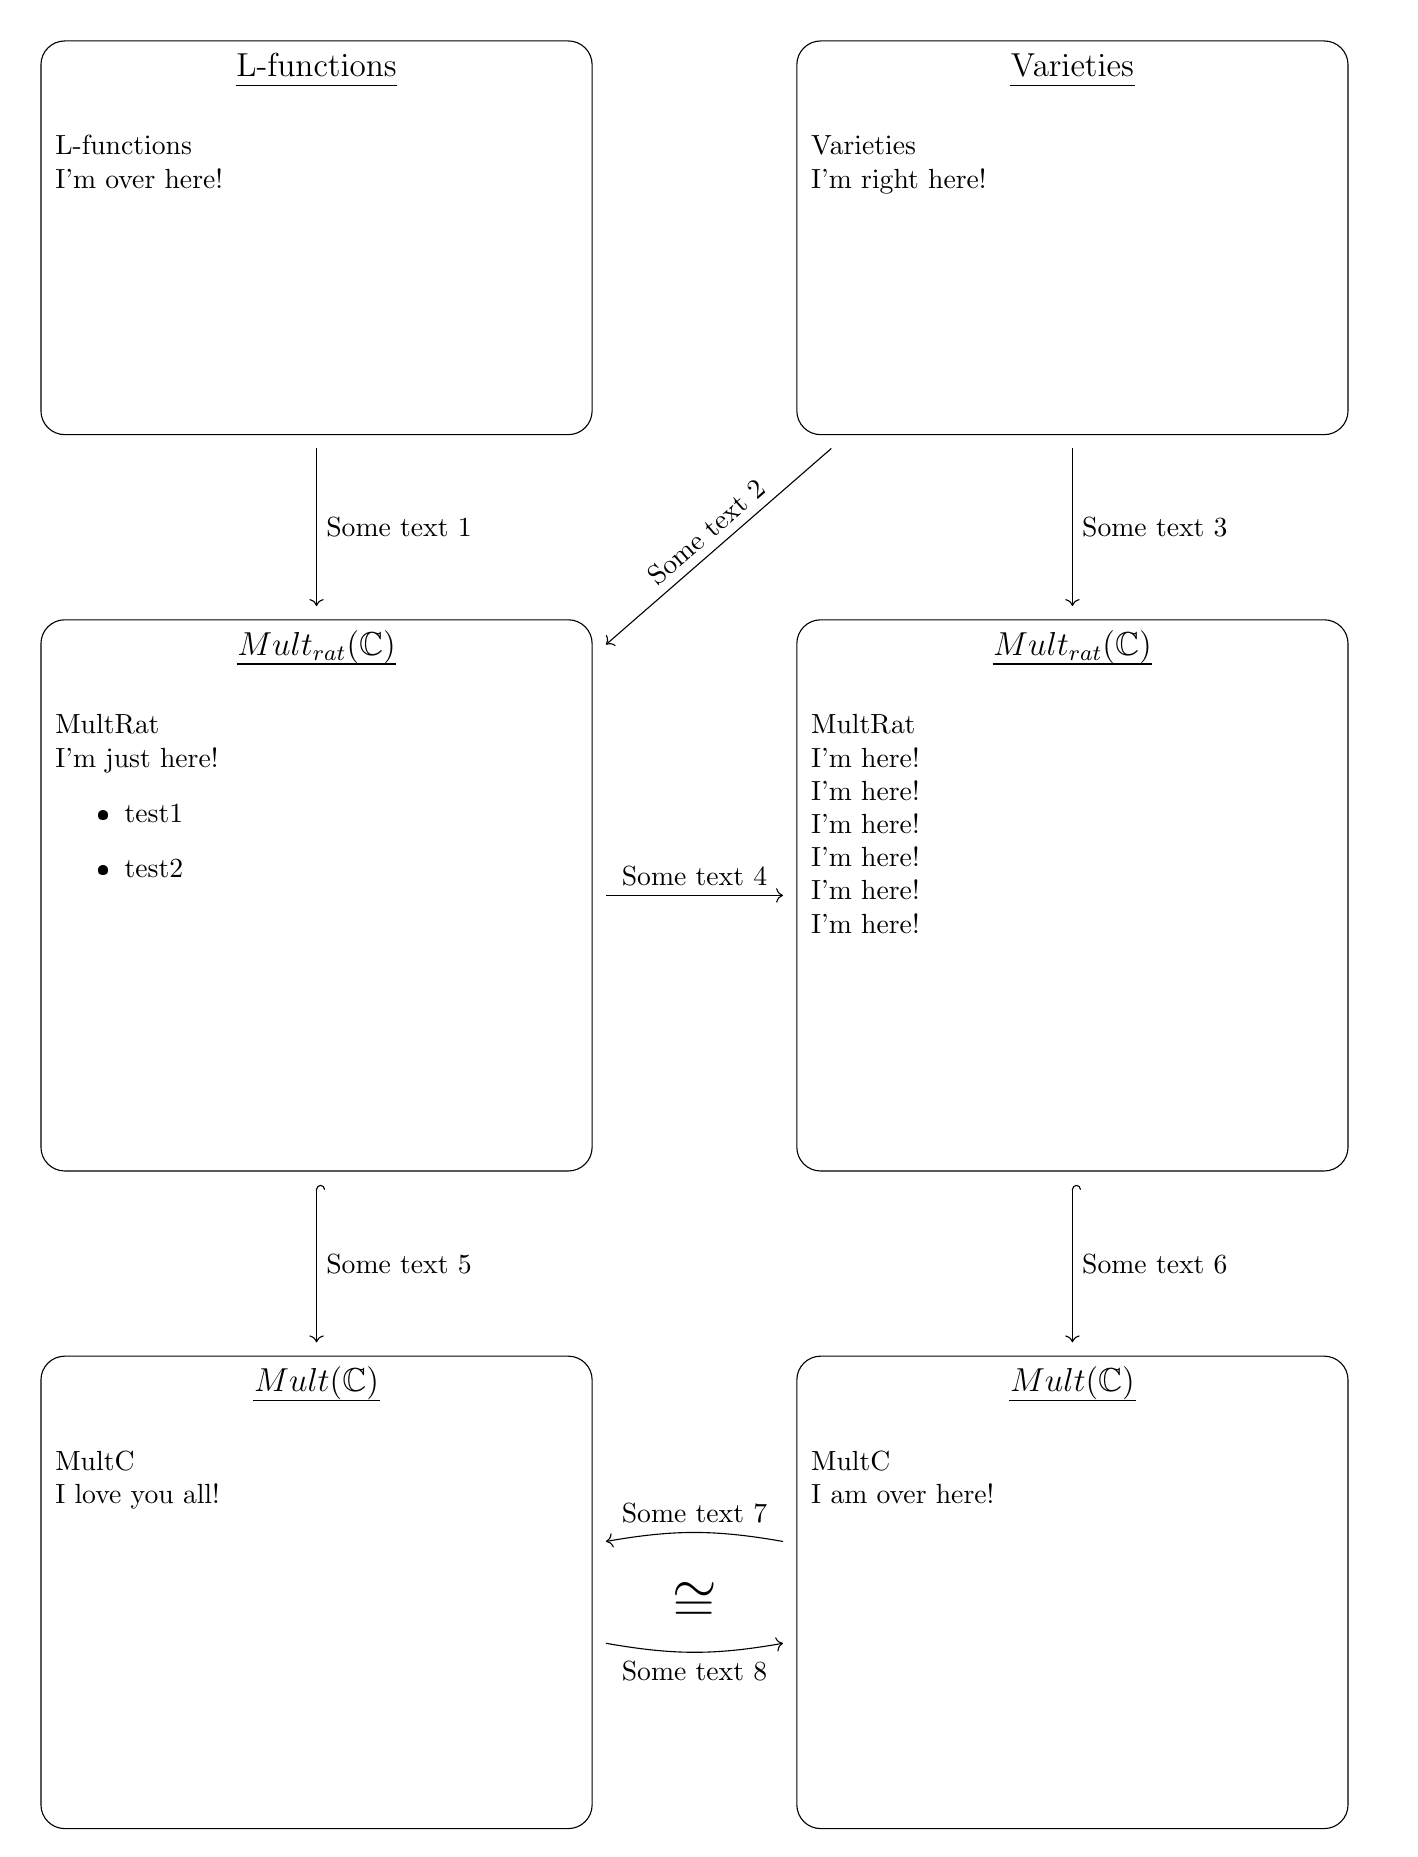
\begin{tikzpicture}[block/.style={draw=black,rounded corners=2ex,minimum width=7cm,minimum height=7cm,outer sep=5pt,inner sep=10pt},content/.style={inner sep=10pt,align=left,below right,text width=7cm},title/.style={align=center,below,font=\large,text height=0.5cm}]

  \node(atcenter) at (0,0) {}; 
  \node(multratbox)   [block,right=1cm of atcenter]{};
  \node(multratcircle)[block,left=1cm  of atcenter]{};
  \node(varieties)    [block,above=2cm of multratbox,minimum height=5cm]{};
  \node(lfunc)        [block,above=2cm of multratcircle,minimum height=5cm]{};
  \node(multcbox)     [block,below=2cm of multratbox,minimum height=6cm]{};
  \node(multccircle)  [block,below=2cm of multratcircle, minimum height=6cm]{};
  
  \node[title]   at (varieties.north){\uline{Varieties}};
  \node[content] at (varieties.north west){\ \\ \ \\ \ \\
  Varieties \\
  I'm right here!
  };
  
  \node[title]   at (lfunc.north){\uline{L-functions}};
  \node[content] at (lfunc.north west){\ \\ \ \\ \ \\
  L-functions \\
  I'm over here!
  };
  
  \node[title]   at (multratcircle.north){\uline{$Mult_{rat}(\C)$}};
  \node[content] at (multratcircle.north west){\ \\ \ \\ \ \\
  MultRat \\
  I'm just here!
  \begin{itemize}
  \item test1 \\
  \item test2
  \end{itemize}
  };
  
  \node[title]   at (multratbox.north){\uline{$Mult_{rat}(\C)$}};
  \node[content] at (multratbox.north west){\ \\ \ \\ \ \\
  MultRat \\
  I'm here! \\
  I'm here! \\
  I'm here! \\
  I'm here! \\
  I'm here! \\
  I'm here!
  };
  
  \node[title]   at (multccircle.north){\uline{$Mult(\C)$}};
  \node[content] at (multccircle.north west){\ \\ \ \\ \ \\
  MultC \\
  I love you all!
  };
  
  \node[title]   at (multcbox.north){\uline{$Mult(\C)$}};
  \node[content] at (multcbox.north west){\ \\ \ \\ \ \\ 
  MultC \\
  I am over here!
  };
  
  \node [below=8.6cm, font=\huge] at (atcenter){$\cong$};
  
  \draw [->] (lfunc)                     -- node [right,midway] {Some text 1} (multratcircle);
  \draw [->] (varieties)                 -- node [above,midway,sloped] {Some text 2} (multratcircle);
  \draw [->] (varieties)                 -- node [right,midway] {Some text 3} (multratbox);
  \draw [->] (multratcircle)             -- node [above,midway] {Some text 4} (multratbox);
  \draw [right hook->] (multratcircle)   -- node [right,midway] {Some text 5} (multccircle);
  \draw [right hook->] (multratbox)      -- node [right,midway] {Some text 6} (multcbox);
  \draw [->,bend right=10] (multcbox)    edge node [above,midway] {Some text 7} (multccircle);
  \draw [->,bend right=10] (multccircle) edge node [below,midway] {Some text 8} (multcbox);

  
\end{tikzpicture}
}



\emph{Rewrite the entire summary AND prelude again after finishing more of the article. Add a comment on Satake parameters for any rational multiplicative function. OR should we just remove the summary - maybe the abstract is enough? We could also add a commutative diagram involving $K_0$, L-functions, Rational multiplicative functions and Multiplicative functions in the first column, and in the second column Satake parameters, Tannakian symbols, and (not connected to Tannakian symbols) Multiplicative functions again, so that the bottom arrow is Bell derivative. Suggestion: Move the norm fixed points to a separate paper.}

Multiplicative functions are ubiquitous in modern number theory. Examples include elementary functions like the Euler totient function, the Liouville function and the M\"obius function, but also a vast class of functions constructed by reading off Dirichlet series coefficients (sometimes called Fourier coefficients) of zeta functions or L-functions with Euler products. We undertake a detailed study of the set of all (complex-valued) multiplicative functions, focussing on algebraic structures naturally occurring on this set, coming from operations such as Dirichlet convolution, natural (pointwise) product, precomposition with a power function, and various operations inspired by algebraic geometry and the theory of L-functions. 
%We have two main results, and two main applications. 

The first main result is a series of theorems equipping the set of multiplicative functions with two distinct but closely related commutative ring structures, each of which is further refined into two distinct but closely related Adams algebra structures. The term ``Adams algebra" is defined in section ??, and is essentially the same thing as Grothendieck's notion of a special lambda-ring. We define an important class of (binary and unary) operations on multiplicative functions called \emph{prime-agnostic operations}, and prove that the four lambda-ring structures taken together neatly encapsulate all prime-agnostic operations on multiplicative functions that we have been able to find in the number theory literature. The four main binary operations in question are Dirichlet convolution, unitary convolution, pointwise product, and a new operation called the tensor product. The unary operations include (but are not limited to) precomposition with a power function, the higher norm operators of Redmond and Sivaramakrishnan, as well as operations derived from base change on schemes over finite fields, and \ldots explain also for example the relation to Rankin-Selberg convolution of automorphic L-functions.

Among the four lambda-ring structures just mentioned, one is more significant than the others, and this structure is referred to as the \emph{standard} lambda-ring structure. Arithmetic geometry is to a large extent concerned with certain Tannakian categories, whose objects give rise to L-functions. Examples include motives, Galois representations, and automorphic representations. The assignment of an L-function to such an object factors through the Grothendieck ring of the Tannakian category in question. Also, to any L-function (with an Euler product) there is a naturally associated multiplicative function. Combining these observations, we get functions from various Grothendieck rings to the set of multiplicative functions, and these are all expected to be lambda-ring homomorphisms with respect to the standard lambda-ring structure (but not with respect to the other three). 

Our second main result is the construction of a new transform from the set of multiplicative functions with rational Bell series to a set of \emph{Tannakian symbols} (a new construct which by imprecise analogy relates to the theory of lambda-rings in the same way as the concept of a matrix relates to the theory of associative algebras). The point of this transform is that it allows for explicit and efficient computations in the lambda-rings just described.

As our first application, we show that our methods yield easy proofs of all known classical identities between multiplicative functions, the only exception we are aware of being the strange identities between divisor functions traditionally derived from finite-dimensionality of spaces of modular forms. %We think of this application as the beginning of a systematic theory of identities between multiplicative functions.

A second application is a series of explicit structure theorems for some of the smallest sub-lambda-rings of the standard lambda-ring structures. These sub-lambda-rings contain the classical multiplicative functions typically encountered in textbooks on elementary number theory, such as the Liouville function, the divisor functions, the Euler totient functions and the M\"obius function. The structure theorems make use of a functorial correspondence between commutative monoids and certain lambda-rings; as an example we mention that [insert example here using the additive monoid of natural numbers]. We think of these theorems as baby cases of a very general approach to structure theory for Grothendieck rings of Tannakian categories.

\emph{We could add here further comments on how Tannakian symbols provide structure and cognitive easing in the general theory of multiplicative functions, but maybe we have said enough already.}

Some of our motivational examples come from algebraic geometry and the theory of L-functions, but we want to emphasize that the main theorems and their proofs, as well as the main applications, are all of an elementary nature in the sense that they rely on nothing more than the definition of a lambda-ring, the definition of a functor, and basic facts from linear algebra and the theory of formal power series.

\subsection{Prelude}

The Laplace transform takes a problem from the world of differential equations and transforms it, almost as by magic, into an the world of algebraic equations, where the problem can be solved and the solution then translated back into the original world. The usefulness of this transform is entirely due to the fact that operations in the first world (such as convolution or differentiation) are transformed into operations in the second world which are familiar and easy to express with explicit formulas.

In a similar spirit, we develop in this paper a machine which takes an identity in the world of multiplicative functions and transforms it into an equivalent identity between \emph{Tannakian symbols}. The latter kind of identity is in almost every case far easier to prove, and the conclusion that the identity is true can be transferred back into the world of multiplicative functions.

We shall explain all this in detail, but in order to convey the flavour of our techniques, we begin by presenting three concrete examples. 

\begin{example}
The Euler totient function is defined by
$$  \varphi(n) = \textrm{the number of integers $x$ such that $1 \leq x \leq n$ and $gcd(x, n) = 1$}  $$

From this explicit definition, we can easily compute values of $\varphi(n)$ for small $n$, and we get the following table:

\vspace{6pt}
\begin{tabular}{  | c || c | c | c | c | c | c | c | c | c | c | c | c | c | c |  }
  \hline			
  $n$ & 1 & 2 & 3 & 4 & 5 & 6 & 7 & 8 & 9 & 10 & 11 & 12 & \ldots & 20  \\
  \hline
  $\varphi(n) $ & 1 & 1 & 2 & 2 & 4 & 2 & 6 & 4 & 6 & 4 & 10 & 4 & \ldots & 8  \\
  \hline  
\end{tabular}
\vspace{6pt}

Are there any patterns here? Well, there may be many, but one particular pattern can be found by choosing a number $n$ (let us choose \underline{the number 6}), and looking at all the function values of \emph{divisors} of 6. The divisors are 1, 2, 3 and 6, and the corresponding function values (circled below) are 1, 1, 2, and 2. Now take the sum of the function values. We get the number 6!

\vspace{6pt}
\begin{tabular}{  | c || c | c | c | c | c | c | c | c | c | c | c | c | c | c |  }
  \hline			
  $n$ & \bf{1} & \bf{2} & \bf{3} & 4 & 5 & \bf{6} & 7 & 8 & 9 & 10 & 11 & 12 & \ldots & 20  \\
  \hline
  $\varphi(n) $ & \raisebox{.5pt}{\textcircled{\raisebox{-.9pt} {1}}} & \raisebox{.5pt}{\textcircled{\raisebox{-.9pt} {1}}} & \raisebox{.5pt}{\textcircled{\raisebox{-.9pt} {2}}} & 2 & 4 & \raisebox{.5pt}{\textcircled{\raisebox{-.9pt} {2}}} & 6 & 4 & 6 & 4 & 10 & 4 & \ldots & 8  \\
  \hline  
\end{tabular}
\vspace{6pt}

Doing the same again, but with \underline{the number 20}, we get the divisors 1, 2, 4, 5, 10 and 20, and the corresponding function values are 1, 1, 2, 4, 4 and 8. 

\vspace{6pt}
\begin{tabular}{  | c || c | c | c | c | c | c | c | c | c | c | c | c | c | c |  }
  \hline			
  $n$ & \bf{1} & \bf{2} & 3 & \bf{4} & \bf{5} & 6 & 7 & 8 & 9 & \bf{10} & 11 & 12 & \ldots & \bf{20}  \\
  \hline
  $\varphi(n) $ & \raisebox{.5pt}{\textcircled{\raisebox{-.9pt} {1}}} & \raisebox{.5pt}{\textcircled{\raisebox{-.9pt} {1}}} & 2 &  \raisebox{.5pt}{\textcircled{\raisebox{-.9pt} {2}}} &  \raisebox{.5pt}{\textcircled{\raisebox{-.9pt} {4}}} & 2 & 6 & 4 & 6 &  \raisebox{.5pt}{\textcircled{\raisebox{-.9pt} {4}}} & 10 & 4 & \ldots &  \raisebox{.5pt}{\textcircled{\raisebox{-.9pt} {8}}}  \\
  \hline  
\end{tabular}
\vspace{6pt}

Their sum is... tadaa... 20!

We are led to believe that there is a general law here, which says that the sum of the values of the Euler function over the divisors of a given integer is precisely that given integer. This statement can be rewritten as an identity:
\begin{equation} \label{introexample1}
\sum_{d \vert n} \varphi(d) = n  
\end{equation}
There are several ways of proving this identity, but we want to give a proof that uses the new machinery introduced in this paper. We first note that $\varphi$ is a multiplicative function whose Tannakian symbol is $\frac{ \{ p  \} }{ \{  1 \}  }$, and that the identity function is also multiplicative, with Tannakian symbol $\frac{ \{ p  \} }{ \varnothing  }$. The left hand side is the M{\"o}bius transform of $\varphi$, and taking the M{\"o}bius transform of a multiplicative function corresponds to adding the Tannakian symbol $\frac{ \{ 1  \} }{ \varnothing } $. The identity (\ref{introexample1}) is therefore equivalent to the statement 
\begin{equation}
\frac{ \{ p  \} }{ \{  1 \}  } \oplus \frac{ \{ 1  \} }{ \varnothing  } = \frac{ \{ p  \} }{ \varnothing  }
\end{equation}
which is obviously true by the general rules for adding two Tannakian symbols. Hence the original identity is proved.
\end{example}


\begin{example}
Let us look at a more complicated example, this time involving an identity which was proved by ?? in ??. The $\tau$ function counts the number of positive divisors of a positive integer $n$. The table of values begins like this:

\vspace{6pt}
\begin{tabular}{  | c || c | c | c | c | c | c | c | c | c | c | c | c | c | c | c | c |  }
  \hline			
  $n$ & 1 & 2 & 3 & 4 & 5 & 6 & 7 & 8 & 9 & 10 & 11 & 12 & .. & 16 & .. & 25  \\
  \hline
  $\tau(n) $ & 1 & 2 & 2 & 3 & 2 & 4 & 2 & 4 & 3 & 4 & 2 & 6 & .. & 5 & .. & 3  \\
  \hline  
\end{tabular}
\vspace{6pt}

Now take any integer - for example \underline{the number 4}. Square the number - in our case we get 16. Now let's play a game with the divisors of 16 (which are 1, 2, 4, 8 and 16). Consider the alternating sum
$$    \tau(1) \cdot \tau(16) -  \tau(2) \cdot \tau(8) + \tau(4) \cdot \tau(4) - \tau(8) \cdot \tau(2) + \tau(16) \cdot \tau(1)  $$
If we plug in the values of the $\tau$ function here, we see that the sum is equal to $\tau(4)$.

Let's try again. We pick \underline{the number 5}, and compute
$$    \tau(1) \cdot \tau(25) -  \tau(5) \cdot \tau(5) + \tau(25) \cdot \tau(1) $$
This sum is equal to \ldots drum roll \ldots $\tau(5)$!
The pattern we see here can be generalized to any $n$, providing we take care in the placement of plus and minus signs in the sum. If we denote by $\Omega(n)$ the number of prime factors of $n$ counted with multiplicity (so that $\Omega(4) = \Omega(6) = 2$ and $\Omega(8) = 3$), then the general identity is
\begin{equation} \label{introexample2}
\sum_{d \vert n^2} (-1)^{\Omega(d)} \tau(d) \tau(\frac{n^2}{d}) = \tau(n)  
\end{equation}
Let us prove it. The $\tau$ function is multiplicative, and its Tannakian symbol is $\frac{ \{ 1 ,1 \} }{ \varnothing }$. The left hand side is what Redmond and Sivaramakrishnan \cite{} call the \emph{norm operator} applied to $\tau$, and in our new language, this is an example of an \emph{Adams operation}, for which we have a simple formula (in the world of Tannakian symbols). This particular Adams operation acts by squaring all elements of the symbol, so the left hand side of the identity is 
$$\frac{ \{ 1^2, 1^2  \} }{ \varnothing  }$$
while the right hand side is 
$$ \frac{ \{ 1, 1  \} }{ \varnothing  } $$
Now the identity follows immediately from the elementary fact that $1 \cdot 1 = 1$. 
\end{example}

\begin{example}
Finally, let us illustrate the power of our new machinery by an example of a much more general nature. We give ourselves the problem of explicitly classifying \emph{all} multiplicative functions $f$ that satisfies the identity 
\begin{equation} \label{introexample3}
\sum_{d \vert n^2} (-1)^{\Omega(d)} f(d) f (\frac{n^2}{d}) = f(n)  
\end{equation}
for all $n$. One example is the $\tau$ function discussed in the previous example. Can we do this? Yes, we can! (Let's make multiplicative functions great again!) We divide the analysis into three sections, solving the problem first in the class of \emph{all} multiplicative functions, then again the the smaller class of \emph{rational} multiplicative functions, and finally in the even smaller class of \emph{Riemann type} multiplicative functions. We rely on terminology which is only introduced later in the paper, including the \emph{Bell derivative} of a multiplicative function (Definition ??) and the Tannakian symbol of a rational multiplicative function at a prime number. 


\begin{enumerate}
\item First let's work within the entire set $Mult(\C)$ of all multiplicative functions. The identity \ref{introexample3} can be rephrased as 
$$ \adam{2}(f) = f  $$
where $\adam{2}$ is the second Adams operation in the standard lambda-ring structure on the set $Mult(\C)$. Inside this set, we are looking for the eigenspace of $\adam{2}$ which corresponds to the eigenvalue $1$. It is a general principle that a multiplicative function $f$ can be constructed by freely assigning function values at prime power arguments. The eigenvalue equation we are trying to solve imposes some restrictions on this process, which can be given a clear meaning if we focus on constructing the \emph{Bell derivative} $f'$ of $f$. In fact, the eigenvalue equation means precisely that we can freely assign values to $f'(p^e)$ for all primes $p$ and all exponents $e$ which are \underline{odd}. In other words, if we let $U$ be the set of odd positive integers and $\bbP$ be the set of prime numbers, then the process of assigning function values to the derivative gives an isomorphism between the sought-for eigenspace and the set $\C^{\bbP \times U}$ of all functions from the Cartesian product $\bbP \times U$ to the complex numbers. Any specified choice of values for $f'(p^e)$, for all pairs $(p, e)$  with $e$ odd, gives a unique multiplicative function $f$ whose values can be explicitly computed, and any such $f$ satisfies the original identity. Conversely, any $f$ satisfying the identity arises in this way. In this analysis, we have implicitly used the fact that any multiplicative function has a unique Bell derivative and a unique Bell antiderivative (and these are also multiplicative functions). 
 
This solves the problem of classifying the multiplicative functions satisfying the identity (\ref{introexample3}). The mysterious appearance of the set $U$ is immediate from the ``compression'' interpretation of the Adams operation given in Section ??.


\item Suppose we are only interested in multiplicative functions which are \emph{rational} in the sense of Definition ??. Inside this smaller set, we can describe the eigenspace in a different but equally explicit way, by using Tannakian symbols instead of the derivative. In fact, rather than ``eigenspace'' we should now use the word ``eigenmodule'', because after imposing the rationality condition, the set of functions we seek to classify is no longer a complex vector space, but rather a free $\Z$-module (with a natural grading), and to determine the functions belonging to this module, we note that at each prime, the function has a Tannakian symbol satisfying the equation 
$$   \text{Ad}^2(\frac{A}{B}) = \frac{A}{B}   $$
where $A$ and $B$ are finite multisets and $\text{Ad}^2$ is the Adams operation defined in Definition ??. Let $L$ be the set of Tannakian symbols satisfying this equation. A choice of rational multiplicative function in our eigenmodule amounts to a choice of one element of $L$ for each prime number - in other words the set of solutions is in natural bijection with the set $L^{\bbP}$ of functions from $\bbP$ to $L$. 

But what is the structure of $L$? In order to answer this question, we need a few pieces of auxiliary definitions. We define a \emph{root cycle of length $k$} to be any set of distinct non-zero complex numbers with the property the set can be ordered into a finite sequence $\alpha_1, \alpha_2, \ldots, \alpha_k$, such that $\alpha_i^2 = \alpha_{i+1}$ for $i = 1, 2, \ldots, k-1$ and $\alpha_k^2 = \alpha_1$. For example, there is only one root cycle of length $1$ (given by $\alpha_1 = 1$, and one root cycle of length 2, given by $\alpha_1 = \omega$, $\alpha_2 = \omega^2$, where $\omega$ is a primitive third root of unity. In general, every number appearing in a root cycle of length $k$ must be a (not necessarily primitive) $(2^k-1)$'th root of unity.

 Let $L_k$ be the free $\Z$-module on the set of root cycles of length $k$, and let 
$$  L = L_1 \oplus L_2 \oplus L_3 \ldots   $$
be a graded module with elements of $L_k$ placed in degree $k$. The ranks of $L_k$ (i.e. the number of root cycles of length $k$) for small values of $k$ are found in the table below:

\vspace{6pt}
\begin{tabular}{  | c || c | c | c | c | c | c | c | c | c | c | c | c |   }
  \hline			
  $k$ & 1 & 2 & 3 & 4 & 5 & 6 & 7 & 8 & 9 & 10 & 11 & 12   \\
  \hline
  $rank(L_k) $ & 1 & 1 & 2 & 3 & 6 & 9 & 18 & 30 & 56 & 99 & 186 & 335    \\
  \hline  
\end{tabular}
\vspace{6pt}

This sequence of ranks (at least up to $k=12$) happens to correspond precisely to the ranks of the degree $k$ part of a free Lie algebra on a set of generators $x_1, x_2, x_3, x_4, \ldots$ (where the generator $x_i$ is placed in degree $i$ for each positive integer $i$). This is a mystery! Is there a canonical (or natural) Lie algebra structure on our module $L$??? We do not know. If such a Lie algebra structure exists, it would transfer to a natural Lie algebra structure on a rather large class of elementary multiplicative functions. For reference, we mention that the sequence of ranks of such a free Lie algebra is labelled A059966 in OEIS (and is different from A107847, which is also related to roots of unity and agrees with the first sequence up to $k=11$). 

In any case, we have defined the module $L$, and we know that any element $v \in L$ determines a Tannakian symbol $T_v$ in the obvious way - whenever a root of unity $\alpha$ appears in a root cycle which has coefficient $m$ in the element $v$, the number $\alpha$ is included in the Tannakian symbol $T_v$ with multiplicity $m$ (i.e. $m$ copies upstairs if $m$ is positive, and $-m$ copies downstairs if $m$ is negative). Together with the explicit link between Tannakian symbols and rational multiplicative functions, this gives an explicit recipe for constructing every possible rational multiplicative function satisfying the identity (\ref{introexample3}), and as we have already mentioned, these functions are therefore in bijection with the explicit set $L^{\mathbb{P}}$.

\item Finally, if we care only for solutions in multiplicative functions of \emph{Riemann type} (meaning that its Dirichlet series can be expressed in terms of the Riemann zeta function as in Definition ??) then the eigenmodule is even smaller, as the uniformity condition implied by being of Riemann type means that the choice we made in the previous paragraph must be the same for each prime $p$. In other words, the set of solutions is in canonical bijection with the graded module $L$ described above. Of the elementary functions listed in the table of Appendix ??, we see, just by inspection of the Tannakian symbol, that the the following functions are solutions to our original puzzle:
\begin{itemize}
\item The zero function $\zero$, defined by $f(1) = 1$ and $f(n) = 0$ for all $n \geq 2$. 
%\item The constant function $\one$ defined by $f(n) = 1$ for all $n$.
\item The function $\tau_k$ for $k$ a positive integer, which by definition means the function corresponding to the Tannakian symbol $\frac{ \{1, 1, \ldots, 1 \} }{ \varnothing  }$ (with $k$ elements upstairs). For $k=1$, this is the constant function $\one$ defined by $f(n) = 1$. For $k = 2$ we get the classical $\tau$ function (counting the number of positive divisors of $n$), and for larger $k$ we get the function which counts the number of ordered factorizations of $n$ into $k$ factors.
\item The functions $\tau_{-k}$ (for $k$ a positive integer). This is the inverse (with respect to Dirichlet convolution) of $\tau_k$, and as a special case (for $k=1$), we get the The M{\"o}bius $\mu$ function.
\item The characteristic function of cubes, the characteristic function of $7$'th powers, etc (any characteristic function of $m$'th powers where $m$ is of the form $2^k-1$. 
\end{itemize}

The first three sets of functions, which together form the so-called $\tau$ family, can be viewed as the canonical copy of $\mathbb{Z}$ inside $Mult(\C)$, when the latter is equipped with the commutative ring structure defined by the operations $\oplus$ and $\otimes$ of Section 3.??. The first operation here is Dirichlet convolution and the second is an extension (in a precise sense) of the tensor product operation on automorphic representations or motives.

%Among the functions which are \emph{not} solutions to our eigenvector problem, we find for example the Euler $\varphi$ function, the divisor functions $\sigma_k$ for $k \geq 1$, etc.

%\emph{Add the remaining classical functions and emphasize again that we determine if the function solves the eigenvalue problem or not simply by inspecting the Tannakian symbol (no computation involved!)}

\end{enumerate}


\end{example}



\subsection{Acknowledgements}

This article is an extension of a high-school project carried out by the first and third author, and all of us (two students and one teacher) would like to thank Fagerlia Upper Secondary School in {\AA}lesund, Norway, and in particular Ivar Karsten Lerstad and Yngve Omen{\aa}s, for encouragement and good working conditions. We are also indebted to many students, and specifically want to thank Fride Nordstrand Nilsen and Charlotte Lund-Hanssen for their keen interest in zeta functions, Pauline Schulze for making mathematics popular in {\AA}lesund and for inspirational writing about a lemma of Mochizuki, and finally Magnus and Olav Hellebust Haaland for their Sage implementation of the Berlekamp-Massey algorithm, which we have used in many of our computations. 

The second author still feels indebted to Lars Svensson, whose legendary undergraduate lectures in Stockholm gave him the impression that to include the ZFC axioms, modular forms, topos theory and Clifford algebras in a first-year undergraduate calculus course is a perfectly natural thing to do. Without you Lars as a role model, I would probably never have assigned a project on lambda-rings and multiplicative functions to two of my ambitious high-school students.

When it comes to mathematical references, we would like to acknowledge the book of McCarthy \cite{} the Online Encyclopedia of Integer Sequences, and the excellent (but unpublished) survey paper of Mathar \cite{}. These three sources provided us with almost all the examples upon which our results are based.

As emphasized by McCarthy, the history of multiplicative functions is ripe with discovery and rediscovery, and it is possible that some specific cases of the results presented here are already in the literature. The existence of our two commutative ring structures on $Mult(\mathbb{C})$ is almost certainly known, but we have not been able to find a reference. We believe that the existence of natural lambda-ring structures on multiplicative functions is not mentioned anywhere in the literature, but Peter Arndt pointed out to us that Jesse Elliott gave a talk in 2013 \cite{} in which the existence of a single such lambda-ring structure was mentioned. However, Elliott does not seem to relate this lambda-ring structure to previously studied operations from number theory or algebraic geometry.

Say something about Unge Forskere and the original report here. Mention also CICM paper perhaps, and current work in progress by the authors, including automated conjecture-making. 

Say something here about lambda-rings and rational Witt vectors. Give reference to Borger, Grinberg, Yau, and perhaps Scholze-Kucharczyk. Thanks to Marcus Zibrowius for exquisite asparagus and for helping us with formulas for symmetric powers.


\subsection{Notation and terminology}

Throughout the paper, we write $\mathbb{N}$ for the set of \emph{strictly positive} integers. The symbols $\mathbb{Z}$, $\mathbb{Q}$, $\mathbb{R}$, and $\mathbb{C}$ all carry their usual meaning. We use $\mathbb{P}$ to denote the set of prime numbers, and we introduce the notation
$$ \mathbb{PP} = \{ 2, 3, 4, 5, 7, 8, 9, 11, 13, 16, \ldots  \}  $$
for the set of all prime powers, i.e. integers that can be written on the form $p^e$, with $p \in \mathbb{P}$ and $e \in \mathbb{N}$.

When $X$ and $Y$ are sets, we write $Y^X$ for the set of all functions from $X$ to $Y$. If $Y$ in this situation carries some algebraic structure, the set $Y^X$ inherits the same kind of algebraic structure by pointwise operations, and we shall refer to this as the \defhl{pointwise} algebraic structure on $Y^X$.

We write $gcd(m, n)$ or sometimes simply $(m, n)$, for the greatest common divisor of two integers $m$ and $n$. We write $lcm(m, n)$ or simply $[m ,n]$ for their least (strictly positive) common multiple.

If $X$ is a finite set, we write $\# X$ for the number of elements in the set $X$. 


With a few exceptions, we shall systematically employ notation according to the list below. Only the letter $h$ serves double functions - this should not create any confusion.
\todo{Review this list of notation after finishing article.}
\begin{itemize}
\item $f$, $g$, $h$: Unspecified multiplicative functions.
\item Various Greek letters: Specific multiplicative functions.
\item $m$, $n$: Natural numbers, either given as arguments to a multiplicative function or used in some other context.
\item $k$ (and occasionally also $h$): Integer parameter indexing a family of multiplicative functions or a family of lambda-ring operations (Example: The divisor functions $\sigma_k$).
\item $r$ will be a real parameter, and $z$ will be a complex parameter.
\item $p$ will always denote a prime, and $e$ will be an exponent. A prime power will be denoted by $p^e$ or occasionally by the letter $q$.
\item $X$ and $Y$ will be sets, sometimes perhaps equipped with some algebraic structure. (\emph{Are these letters actually used??}
\item Notation for monoids? $M$ and $N$?
\item $A$, $B$, $C$ and $D$ will be multisets.
\item $\alpha_i$ and $\beta_j$ will be elements (usually complex numbers) of some multiset. Usually $i$ will go from 1 to $m$ and $j$ will go from $1$ to $n$.
\item Explain convention that elements from $A$ belongs to the denominator etc???
\item Coefficients of a power series $c_1$, $c_2$, etc, or do we also need $a_i$ and $b_i$? Or some other notation, like capital letters???
\item $t$ will be the formal variable in a formal power series, and $s$ will be the formal variable in a formal Dirichlet series.
\item $R$ will be a ring. Sometimes we shall use $Z$ and $Q$, explain why.
\item Given $R$ (ring or semiring), we write $R_{add}$ and $R_{mult}$ for the underlying monoids of $R$. I think this is best, then we can add a condition as superscript, like in $\mathbb{R}_{add}^{\geq 0}$.
\item If $f$ is a multiplicative function, its Bell derivative will be denoted by $f'$ or sometimes by $\BD f$. 
\item Symmetric operations will be denoted by three- or four-letter abbreviations, such as $Ext$, $Sym$, etc (review this decision and add newcommands!!)
\item $T$ and $S$ will be Tannakian symbols.
\item Surely there are letters we have forgotten. 
\item $a$, $b$, $c$ will be elements of the multisets appearing in Tannakian symbols.
\end{itemize}



Explain the notation and terminology related to "box" and "circle"?

Finally, we mention that in addition to Appendix ?? on Adams operations, we have also included appendices ??, ?? and ?? which together give an overview of the plethora of functions, operations, classes of functions and classes of operations. For a serious reader it might be helpful to keep a print copy of all these appendices at hand while reading the remainder of the article.

\emph{Fix conventions for font styles of functors, operations on power series, operations on lambda-rings, operations of multiplicative functions (maybe not) and the multiplicative functions themselves.}

A few of the operations on multiplicative functions which we found in the literature did not have any names in the sources we consulted, and in these cases we have introduced names which seem reasonable. Same is true for operations, and this concerns the Schemmel transform, the LCM convolution, the GCD transform, the $k-$twisted convolution and ???

The most challenging aspect of choosing notation is that there are so many Adams operations around. Explain double usage??? Print appendix!


We now collect the definitions we use from abstract algebra:

Define relevant categories?

Add here brief intro to monoids/commutative monoids. Rings/commutative rings. Follow CICM paper perhaps. Or refer to other sources and skip this stuff here.

Define binomial coefficient, define binomial ring?

Explain what it means for a map to commute with an operation.


\subsection{Prerequisites}

Some of our constructions are inspired by notions from algebraic geometry (such as schemes, varieties, base change and Weil restriction) and notions from representation theory and analytic number theory (such as automorphic L-functions, Tannakian categories, and the canonical lambda-ring structure on the Grothendieck ring of any Tannakian category). From a logical point of view however, the definitions and results of the present paper do not rely on any material from these fields of study beyond a superficial familiarity with the words ``category'' and ``functor''.

We hope that the structure of the presentation makes all the results accessible to anyone with some basic knowledge of elementary number theory and abstract algebra, while at the same time making clear to experts (by way of examples) what the connections are to algebraic geometry and to the theory of motivic and automorphic L-functions. 

In order to explain the connections to algebraic geometry without relying on the full machinery of commutative algebra and locally ringed spaces, we have presented a small didactical experiment in Section ??, where we introduce the notion of a \emph{micro-scheme}. A micro-scheme is any machine that takes a finite ring as input and gives a finite set as output. These machines may serve as a high-school teacher's substitute for schemes in the sense of Grothendieck.

\subsection{The scope of this article}

Goals: (1) Language and (2) Application to algebraic structure on multiplicative functions.

Leaving out: (1) Details on many other applications (see future publications), (2) Rings which are not subrings of $\C$, and (3) Metric structures.

Explain/justify why we work with complex-valued functions? Domain? Field? Alg closed? Q-algebra? Give ref to general discussion in endnotes. Mention somewhere p-adic modular forms/p-adic L-functions, and also dual numbers and Tao's ideas, as possible applications of more general target rings.

Mention that we introduce many topics which we intend to treat in more detail in future work. In particular, connections to the ideas of Tao on derived multiplicative functions.

Mention also the Endnotes, where we sum up what remains to be done.




\section{Multiplicative functions and the Bell derivative}

In this section we give basic definitions and some examples of multiplicative functions. Two key definitions (which we believe are new) are (1) the definition of the \emph{Bell derivative} $f'$ of a multiplicative function $f$, and (2) the definition of  a \emph{rational} multiplicative function.

\subsection{Multiplicative functions}

Recall that $\N$ in this paper denotes the set of \emph{strictly positive} integers.

\begin{definition}
A function from $\N$ to $\C$ is called an \defhl{arithmetical function}.
\end{definition}

\begin{definition} \label{def:multiplicative}
A arithmetical function $f: \mathbb{N} \to \mathbb{C}$ is called a \defhl{multiplicative function} if it satisfies the two conditions
\begin{itemize}
\item[(i)] $f(1) = 1$
\item[(ii)] $f(mn) = f(m) f(n)$ for all $m, n$ which are coprime.
\end{itemize}
A multiplicative function is \defhl{completely multiplicative} if the second condition holds for \emph{all} $m, n$ in $\N$.

\end{definition}

%\begin{definition}
%\emph{Define Dirichlet convolution and Dirichlet inverse here? Also define totient and specially multiplicative, and add comments about these notions when appropriate throughout this section?}
%\end{definition}

%\begin{definition}
%(Copied from a later section) Let $f$ and $g$ be two multiplicative functions. We define the \defhl{Dirichlet convolution} of $f$ and $g$ (denoted here by $f \oplus g$ instead of the more traditional $f * g$) by the formula
%$$ (f \oplus g)(n) =  \sum_{d \vert n} f(d) g(n/d)  $$
%Here the sum on the right hand side is taken over all positive divisors $d$ of $n$. The reason for introducing non-standard notation is that we want to think of Dirichlet convolution as an additive rather than as a multiplicative operation.
%\end{definition}

\begin{example}
In the Prelude, we encountered the Euler totient function $\varphi$, as well as the $\tau$ function (the latter may be denoted by $d$ or $\sigma_0$ in some sources). Recall that $\varphi(n)$ is the number of positive integers smaller than or equal to $n$ which are coprime to $n$, and that $\tau(n)$ is the number of positive divisors of $n$. Both the Euler function and the $\tau$ function are multiplicative functions but \emph{not} completely multiplicative.
\end{example}

\begin{definition}
We give only two examples of functions which are arithmetical but not multiplicative. We define $\omega(n)$ to be the number of distinct prime factors of $n$, and we define $\Omega(n)$ to be the number of prime factors \emph{counted with multiplicity}. In other words, if
$$ n = p_1 ^{e_1} p_2^{e_2} \cdots p_m^{e_m}  $$
is the unique prime factorization of the number $n$, then
$$ \omega(n) = m    $$
and
$$  \Omega(n) = \sum_{i=1}^m  e_i $$
\end{definition}

\begin{example}
The Liouville function $\lambda$ is defined by the formula
$$ \lambda(n) = (-1)^{\Omega(n)}  $$
It is a completely multiplicative function.
\end{example}

\begin{definition}
A number $d$ is \defhl{square-free} if no square number except $1$ is a divisor of $d$.
\end{definition}

\begin{example}
We define $\Theta(n)$ to be the number of square-free divisors of $n$. The function $\Theta$ is multiplicative but not completely multiplicative. One can show that the relation
$$ \Theta(n) = 2^{\omega(n)}   $$
holds.
\end{example}

We remind the reader that Appendix ?? contains an overview of all multiplicative functions appearing in this paper.

\begin{definition}
We define $Mult(\mathbb{C})$ to be \defhl{the set of all multiplicative functions}. We define $CMult(\mathbb{C})$ to be \defhl{the set of all completely multiplicative functions}.
\end{definition}

Any multiplicative function $f$ is determined by its values on the set $\PP$ of prime powers. The reason is that if $n$ is a positive integer, we can factor $n$ as $p_1^{e_1} p_2^{e_2} \cdots p_m^{e_m}$, and because $f$ is multiplicative, we have
$$ f(n) = f(p_1^{e_1}) f( p_2^{e_2}) \cdots f(p_m^{e_m})   $$
On the other hand, we can construct a multiplicative function by assigning an arbitrary function value to each prime power, and then extend the function to all positive integers by the above formula.

Similarly, a completely multiplicative function is determined by its values on the set $\bbP$ of prime numbers, since for such a function we always have
$$  f(n) = f(p_1)^{e_1} f( p_2)^{e_2} \cdots f(p_m)^{e_m}  $$

We reformulate and record these two elementary and well-known observations in a lemma, for later use. Recall that $Y^X$ denotes the set of all functions from the set $X$ to the set $Y$.


\begin{lemma} \label{AffineSpaceLemma}
\begin{itemize}
\item[i)] Consider the composition
$$ Mult(\C) \rightarrow \C^{\N} \rightarrow \C^{\PP}   $$
where the first arrow is the obvious inclusion, and the second arrow is given by restriction from the set $\N$ to its subset $\PP$. This composition is a bijection.
\item[ii)] Consider the composition
$$ CMult(\C) \rightarrow \C^{\N} \rightarrow \C^{\bbP}   $$
where the first arrow is the obvious inclusion, and the second arrow is given by restriction from the set $\N$ to its subset $\bbP$. This composition is also a bijection.
\end{itemize}
\end{lemma}

\begin{definition}
The map from $Mult(\C)$ to $\C^{\PP}$ described in the Lemma will be referred to as \defhl{the canonical bijection} between these two sets.
\end{definition}

\begin{definition}
(Informal) Let $f$ be a multiplicative function. A \defhl{master equation} for $f$ is a formula for the function value $f(p^e)$, valid for all primes $p$ and all positive integers $e$.
\end{definition}

\begin{example}
The Euler function has master equation
$$ \varphi(p^e) = p^e - p^{e-1}   $$
while the $\tau$ function has master equation given by
$$ \tau(p^e) = e+1  $$
\end{example}

\begin{example}
The Liouville function has the master equation
$$ \lambda(p^e) = (-1)^e  $$
and the function $\Theta$ has master equation
$$ \Theta(p^e) = 2   $$
\end{example}

We now collect a few definitions related to various generating series constructed from multiplicative functions. They will play a central role in many of our constructions and proofs.

\begin{definition}
Let $f$ be a multiplicative function, and let $p$ be a prime. The \defhl{Bell series of $f$ at $p$} is the formal power series
$$ 1 + f(p) \ t + f(p^2) \ t^2 + f(p^3) \ t^3 + \ldots    $$
Here $t$ is a formal variable, and the series is an element of the formal power series ring $\mathbb{C}[[t]]$.
\end{definition}

\begin{remark}
By Lemma \ref{AffineSpaceLemma}, a multiplicative function is fully determined by its Bell series at all primes (taken together).
\end{remark}

\begin{definition}
The number $f(p^e)$ is called the \defhl{Bell coefficient} at the prime power $p^e$.
\end{definition}

The values $f(n)$ may be tabulated in the usual ``linear'' way, as we did for the Euler totient function once already:

\vspace{6pt}
\begin{tabular}{  | c || c | c | c | c | c | c | c | c | c | c | c | c | c | c |  }
  \hline
  $n$ & 1 & 2 & 3 & 4 & 5 & 6 & 7 & 8 & 9 & 10 & 11 & 12 & \ldots & 20  \\
  \hline
  $\varphi(n) $ & 1 & 1 & 2 & 2 & 4 & 2 & 6 & 4 & 6 & 4 & 10 & 4 & \ldots & 8  \\
  \hline
\end{tabular}
\vspace{6pt}

However, this display hides many of the patterns in the function values, and it is often better to tabulate only the function values $f(p^e)$ in a two-dimensional array indexed by the prime $p$ and the exponent $e$. Here is what happens for the Euler function:

\begin{center}
\begin{tabular}{| l | | c | c | c | c | c | c |}
\hline
& $e = 1$ & $e = 2$ & $e = 3$ & $e = 4$ & $e = 5$ & $e = 6$ \\
\hline
\hline
$p = 2$ & 1 & 2 & 4 & 8 & 16 & 32 \\
\hline
$p = 3$ & 2 & 6 & 18 & 54 & 162 & 486 \\
\hline
$p = 5$ & 4 & 20 & 100 & 500 & 2500 & 12500 \\
\hline
$p = 7$ & 6 & 42 & 294 & 2058 & 14406 & 100842 \\
\hline
\end{tabular}
\end{center}

In this particular case, we easily see that the rows form geometric sequences, and it is easy to read off the pattern both in the initial terms and in the successive quotients of these sequences.

\begin{definition}
(Informal) If $f$ is any multiplicative function, we use the word \defhl{Bell table} for a two-dimensional table of the function values $f(p^e)$, indexed by $p$ and $e$, as above.
\end{definition}

\begin{example}
The Bell table of the Liouville function:
\vskip10pt
\begin{center}
\begin{tabular}{| l | | c | c | c | c | c |}
\hline
& $e = 1$ & $e = 2$ & $e = 3$ & $e = 4$ & $e = 5$\\
\hline
\hline
$p = 2$ & -1 & 1 & -1 & 1 & -1 \\
\hline
$p = 3$ & -1 & 1 & -1 & 1 & -1 \\
\hline
$p = 5$ & -1 & 1 & -1 & 1 & -1 \\
\hline
$p = 7$ & -1 & 1 & -1 & 1 & -1 \\
\hline
\end{tabular}
\end{center}
\end{example}

\begin{example}
The Bell table of the $\Theta$ function:
\vskip10pt
\begin{center}
\begin{tabular}{| l | | c | c | c | c | c |}
\hline
& $e = 1$ & $e = 2$ & $e = 3$ & $e = 4$ & $e = 5$\\
\hline
\hline
$p = 2$ & 2 & 2 & 2 & 2 & 2 \\
\hline
$p = 3$ & 2 & 2 & 2 & 2 & 2 \\
\hline
$p = 5$ & 2 & 2 & 2 & 2 & 2 \\
\hline
$p = 7$ & 2 & 2 & 2 & 2 & 2 \\
\hline
\end{tabular}
\end{center}
\end{example}

\begin{example}
The Bell table of the $\tau$ function:
\vskip10pt
\begin{center}
\begin{tabular}{| l | | c | c | c | c | c |}
\hline
& $e = 1$ & $e = 2$ & $e = 3$ & $e = 4$ & $e = 5$\\
\hline
\hline
$p = 2$ & 2 & 3 & 4 & 5 & 6 \\
\hline
$p = 3$ & 2 & 3 & 4 & 5 & 6 \\
\hline
$p = 5$ & 2 & 3 & 4 & 5 & 6 \\
\hline
$p = 7$ & 2 & 3 & 4 & 5 & 6 \\
\hline
$p = 11$ & 2 & 3 & 4 & 5 & 6 \\
\hline
\end{tabular}
\end{center}
\end{example}


\begin{example}
Let $\tau_k(n)$ be the number of ordered factorizations of $n$ into $k$ factors. Then $\tau_k$ is a multiplicative function. For $k=2$ we recover the $\tau$ function from earlier.

Here is the Bell table for $\tau_4$:
\vskip10pt
\begin{center}
\begin{tabular}{| l | | c | c | c | c | c |}
\hline
& $e = 1$ & $e = 2$ & $e = 3$ & $e = 4$ & $e = 5$\\
\hline
\hline
$p = 2$ & 4 & 10 & 20 & 35 & 56 \\
\hline
$p = 3$ & 4 & 10 & 20 & 35 & 56 \\
\hline
$p = 5$ & 4 & 10 & 20 & 35 & 56 \\
\hline
$p = 7$ & 4 & 10 & 20 & 35 & 56 \\
\hline
$p = 11$ & 4 & 10 & 20 & 35 & 56 \\
\hline
\end{tabular}
\end{center}
We recognize the numbers here from the 4'th diagonal of Pascal's triangle, and indeed the general master equation is
$$ \tau_k(p^e) =  \binom{k-1+e}{e}  $$
where the right hand side is a binomial coefficient.
\end{example}


\begin{definition}
Let $f$ be any function from $\N$ to $\C$. The \defhl{Dirichlet series} associated to $f$ is the formal series
$$  D_f(s) = \sum_{n=1}^{\infty} f(n) n^{-s}   $$

If $f$ is multiplicative, then the Dirichlet series of $f$ can be rewritten as a (formal) product over all prime numbers:
$$  D_f(s) = \prod_p f_p(p^{-s})   $$
where $f_p$ is the Bell series of $f$ at $p$. Any formal product of this form (with $f_p$ a formal power series with complex coefficients) is called an \defhl{Euler product}, and the expression $f_p(p^{-s})$ is called the \defhl{Euler factor} at the prime $p$.

Conversely, let $D(s) = \sum a_n n^{-s} = $ be a Dirichlet series admitting an Euler product. The function  $f(n) = a_n$ is then multiplicative, and we refer to it as the \defhl{underlying multiplicative function} of $D(s)$.
\end{definition}

\begin{example}
The constant multiplicative function (all of whose function values are equal to $1$) will be denoted by $\one$. Its Dirichlet series is the Riemann zeta function $\zeta(s)$.
\end{example}

\begin{example}
The multiplicative function defined by the master equation $f(p^e) = 0$ will be denoted by $\zero$. Its Dirichlet series is equal to 1. Note that $\zero(1) = 1$, while $\zero(n) = 0$ for all $n \geq 2$.
\end{example}

\begin{example}
Here are the Dirichlet series for the other functions encountered so far:
\begin{itemize}
\item $D_{\Theta}(s) = \frac{\zeta(s)^2}{\zeta(2s)}$
\item $D_{\tau}(s) = \zeta(s)^2$
\item $D_{\lambda}(s) = \frac{1}{\zeta(s)}$
\item $D_{\varphi}(s) = \frac{\zeta(s - 1)}{\zeta(s)}$
\end{itemize}
The function $\tau_k$ has Dirichlet series $\zeta(s)^k$.
\end{example}



\begin{example}
In many real-life examples of Dirichlet series admitting an Euler product, each Euler factor is of the form ${1} / {L_p(p^{-s})}$ with $L_p$ a polynomial, and this degree of this polynomial is often the same for all but a finite number of primes $p$. In this situation, the primes in the finite set of exceptions are referred to as \emph{bad primes}. For example, any \emph{automorphic L-function} is of this form, and the same is true for any L-function associated to a Galois representation, or to a motive (assuming the motive is pure of some specific weight). In general the existence of these L-functions means that we can speak of \emph{the multiplicative function associated to} an automorphic representation, a Galois representation or a motive.
\end{example}

\begin{example}
To take a specific example of automorphic nature, we consider the famous modular form $\Delta$, whose coefficients are given by the Ramanujan $\tau$ function (not to be confused with the $\tau$ function above). Its Bell table looks like this:
\vskip10pt
\begin{center}
\begin{tabular}{| l | | c | c | c | c |}
\hline
& $e = 1$ & $e = 2$ & $e = 3$ & $e = 4$ \\
\hline
\hline
$p = 2$ & -24 & -1472 & 84480 & 987136 \\
\hline
$p = 3$ & 252 & -113643 & -73279080 & 1665188361 \\
\hline
$p = 5$ & 4830 & -25499225 & -359001100500 & -488895969711875 \\
\hline
\end{tabular}
\end{center}



\end{example}



\begin{example}
Let $G$ be a $\mathcal{T}$-group, meaning a finitely generated, torsion-free and nilpotent group. Let $a_n$ be the number of subgroups of $G$ of index $n$, and define a function $f_G$ by the formula $f_G(n) = a_n$. Then $f_G$ is multiplicative. A concrete example is the abelian group $\mathbb{Z}^3$. The associated multiplicative function famously has Dirichlet series $\zeta(s) \zeta(s-1) \zeta(s-2)$, and Bell table:
\vskip10pt
\begin{center}
\begin{tabular}{| l | | c | c | c | c | c |}
\hline
& e = 1 & e = 2 & e = 3 & e = 4 & e = 5\\
\hline
\hline
p = 2 & 7 & 35 & 155 & 651 & 2667 \\
\hline
p = 3 & 13 & 130 & 1210 & 11011 & 99463 \\
\hline
p = 5 & 31 & 806 & 20306 & 508431 & 12714681 \\
\hline
p = 7 & 57 & 2850 & 140050 & 6865251 & 336416907 \\
\hline
p = 11 & 133 & 16226 & 1964810 & 237758115 & 28768909071 \\
\hline
\end{tabular}
\end{center}
A more interesting example is the so-called discrete Heisenberg group of $3 \times 3$-upper-unitriangular matrices over the integers, i.e. the multiplicative group of all matrices of the form
$$
\begin{bmatrix}
    1       & a & b  \\
    0       & 1 & c  \\
     0      & 0 & 1
\end{bmatrix}
$$
with $a, b, c \in \mathbb{Z}$. The associated multiplicative function has Dirichlet series
$$ \frac{\zeta(s) \zeta(s-1) \zeta(2s-3) \zeta(2s-2) }{\zeta(3s-3)} $$
and Bell table
\vskip10pt
\begin{center}
\begin{tabular}{| l | | c | c | c | c | c |}
\hline
& $e = 1$ & $e = 2$ & $e = 3$ & $e = 4$ & $e = 5$\\
\hline
\hline
$p = 2$ & $3$ & $19$ & $43$ & $203$ & $427$ \\
\hline
$p = 3$ & $4$ & $49$ & $157$ & $1534$ & $4693$ \\
\hline
$p = 5$ & $6$ & $181$ & $931$ & $24056$ & $120931$ \\
\hline
$p = 7$ & $8$ & $449$ & $3193$ & $159258$ & $1117257$ \\
\hline
$p = 11$ & $12$ & $1585$ & $17557$ & $2140502$ & $23560285$ \\
\hline
\end{tabular}
\end{center}
We have borrowed these examples from Voll \cite{VollIntro}. See also du Sautoy's ICM presentation \cite{duSautoyICM} for an introduction to these ideas and related definitions for certain classes of rings.
\end{example}

In later sections, we shall discuss numerous examples of multiplicative functions of a more elementary nature, but also several different types of multiplicative functions coming from algebraic geometry, including the multiplicative function underlying the Hasse-Weil zeta function of a scheme.

\subsection{Rational multiplicative functions}

Almost all examples of multiplicative functions appearing in number theory and algebraic geometry satisfy a property which we want to call \emph{rationality}.

We shall see later that there is a natural topology on $Mult(\C)$ with the property that the rational multiplicative functions form a dense subset. This observation will lead to very short proofs of many purely algebraic statements.

\begin{definition}
We say that a multiplicative function $f$ is \defhl{rational} if the Bell series $f_p(t)$ is a rational power series for all primes $p$.
\end{definition}

\begin{remark}
A multiplicative function is rational if and only if for every prime number $p$, the sequence
$$ f(p), f(p^2), f(p^3), \ldots  $$
is linearly recursive (these are the sequences occurring as rows in a Bell table for $f$).
\end{remark}

\begin{definition}
We write $Mult_{rat}(\C)$ for the set of all rational multiplicative functions.
\end{definition}

\begin{example}
All the multiplicative functions we have seen so far are rational, including the modular form example, the two examples coming from finitely generated groups, each of the $\tau_k$ functions, the constant function $\one$, the zero function $\zero$ the Euler $\varphi$ function, the Liouville function, and the $\Theta$ function.
\end{example}

Finding example of non-rational multiplicative functions is quite hard, but there will be examples appearing in later sections, including some multiplicative functions underlying zeta functions of \emph{algebraic stacks}. For now we simply give give two examples, first a function which may or may not be rational, and then another function that is provably non-rational.

\begin{example}
Let $f(n)$ be the number of commutative but not necessarily unital rings with $n$ elements. Then $f$ is a multiplicative function, but it is very hard to compute $f(n)$ for large values of $n$. The Bell table looks like this - here question marks indicate that the value of $f(p^e)$ is unknown, and a symbol like $>876$ indicates that the value is unknown but larger than (in this case) 876. The values appearing in the table are taken from OEIS (sequence A037289), and we have not checked the details of the original sources. (It would probably be wise to double-check that none of the numbers 34 and 36 appearing here are misprints in OEIS.)

\begin{center}
\begin{tabular}{| l | | c | c | c | c | c | c | c |}
\hline
& $e = 1$ & $e = 2$ & $e = 3$ & $e = 4$ & $e = 5$ & $e = 6$ & $e=7$ \\
\hline
\hline
$p = 2$ & 2 & 9 & 34 & 162 & $>876$ & $>12696$  & ? \\
\hline
$p = 3$ & 2 & 9 & 36 & ? & ? & ? & ? \\
\hline
$p = 5$ & 2 & 9 & ? & ? & ? & ?  & ?\\
\hline
$p = 7$ & 2 & 9 & ? & ? & ? & ?  & ?\\
\hline
$p = 11$ & 2 & ? & ? & ? & ? & ?  & ?\\
\hline
$p = 13$ & 2 & ? & ? & ? & ? & ?  & ?\\
\hline
$p = 17$ & 2 & ? & ? & ? & ? & ?  & ?\\

\hline
\end{tabular}
\end{center}
\end{example}


\begin{example}
An \defhl{exponential divisor} of a natural number
$$n = p_1^{e_1} \cdot p_2^{e_2} \cdots p_m^{e_m}$$
is an integer of the form
$$ d = p_1^{c_1} \cdot p_2^{c_2} \cdots p_m^{c_m}   $$
where $c_i$ divides $e_i$ for all $i$. Let $f(n)$ be the number of exponential divisors of $n$. Then $f$ is a multiplicative function, with master equation
$$f(p^e) = \tau(e)$$
and OEIS label A049419. To prove that this function is not rational, we argue as follows. Assume that the sequence
$$ f(p), f(p^2), f(p^3), \ldots   $$
is linearly recursive. Subtracting the number 2 from each number in the sequence gives another sequence which also is linearly recursive, whose $k$'th term is
$$  a_k = \tau(k) - 2.  $$
Let $S$ be the set of zeroes of this sequence, i.e. the set
$$ \{ k \in \mathbb{N}  \ \vert \ a_k = 0  \}  $$
The Skolem-Mahler-Lech theorem (Ref. Theorem 2.1, page 25, in Everest et al) says that set of zeroes of any linearly recursive sequence (at least over a field of characteristic zero) is a union of a finite set and a finite number of arithmetic progressions. On the other hand, we see from the definition of the $\tau$ function that the set $S$ is precisely the set of prime numbers. This is a contradiction, and hence the original sequence cannot be linearly recursive.
\end{example}


\subsection{Multiplicative functions with values in other rings}

In the above definitions, we could have replaced $\C$ throughout with any commutative ring $R$. In this way, we obtain the notion of an $R$-valued multiplicative function, and we can form the set $Mult(R)$, the set $CMult(R)$ and the set $Mult_{rat}(R)$. Note that we have inclusions
$$ CMult(R) \hookrightarrow Mult_{rat}(R) \hookrightarrow Mult(R)   $$

As explained in the introduction, this article only considers rings $R$ which are subrings of $\C$. In future work we hope to treat general commutative rings, in particular the rings of dual numbers (and higher analogues) which appear in Tao's approach to derived multiplicative functions.
\begin{definition}
For any function $f$ in $Mult(\C)$, there exists a smallest subring $R$ of $\C$ with the property that $f$ lies in $Mult(R)$. This ring is called the \defhl{coefficient ring} associated to $f$.
\end{definition}

\begin{example}
Any function which \emph{counts} something obviously has coefficient ring $\mathbb{Z}$.
\end{example}


\begin{example}
The $5$-adic absolute value is a multiplicative function. It is defined by the equation
$$   \vert n \vert_5 = 5^{-v_5(n)}  $$
where $v_5(n)$ is the number of copies of $5$ in the prime factorization of $n$. For example, the prime factorization of 650 is $2 \cdot 5 \cdot 5 \cdot  13$, so $v_5(650) = 2$, and the $5$-adic absolute value of 650 is equal to $\frac{1}{25}$.
The Bell table of the $5$-adic absolute value looks like this:
\vskip10pt
\begin{center}
\begin{tabular}{| l | | c | c | c | c | c |}
\hline
& $e = 1$ & $e = 2$ & $e = 3$ & $e = 4$ & $e = 5$\\
\hline
\hline
$p = 2$ & 1 & 1 & 1 & 1 & 1 \\
\hline
$p = 3$ & 1 & 1 & 1 & 1 & 1 \\
\hline
$p = 5$ & 1/5 & 1/25 & 1/125 & 1/625 & 1/3125 \\
\hline
$p = 7$ & 1 & 1 & 1 & 1 & 1 \\
\hline
\end{tabular}
\end{center}
The coefficient ring of this function is $\Z[\frac{1}{5}]$, i.e. the set of all rational numbers which can be written on the form $\frac{a}{b}$, where $b$ is a power of $5$ (with non-negative integer exponent, so $b =1$ is allowed).
\end{example}

\begin{example}
We're not entirely sure about the technical details here, but multiplicative functions coming from automorphic L-functions are either algebraic (in which case we think the coefficient ring is contained in some number field), or non-algebraic, in which case many (all???) of the coefficients in the Bell table are non-algebraic numbers. Some of the simplest non-algebraic examples are given by so-called Maass forms. Here is the Bell table of the Maass form on $\Gamma_0(5)$ with spectral parameter $R \approx 3.02837629307$, with data copied from the LMFDB database. The coefficients here are all rounded to 9 or 10 correct decimals.
\vskip10pt
\begin{center}
\begin{tabular}{| l | | c | c | c | c |}
\hline
& $e = 1$ & $e = 2$ & $e = 3$ & $e = 4$ \\
\hline
\hline
$p = 2$ & -0.593266803 & -0.6480345004 & 0.9777241593 & 0.0679832141 \\
\hline
$p = 3$ & 1.113764923 & 0.2404723031 & -0.8459353058 & -1.1826453656 \\
\hline
$p = 5$ & 0.4472135955 & 0.2 & 0.0894428085 &  \\
\hline
\end{tabular}
\end{center}
The missing digit (for the prime power $5^4$) was not in the LMFDB (they only display the values $a_n$ for $n \leq 500$). We do not know if the number $0.2$ in the table is exactly equal to $\frac{1}{5}$ or if it just happens to be very close; maybe some expert on Maass forms could tell.
\end{example}

\begin{example}
Any Dirichlet character is a multiplicative function, whose coefficient ring is the ring of integers in some cyclotomic number field.
\end{example}

\begin{example}
Let $z$ be a fixed complex number. We write $id_z(n)$ for $n^z$. Then $id_z$ is a completely multiplicative function. We make a few observations, but recall first that when $b$ is a positive real number (for example a positive integer), then the expression $b^z$ is unambiguously defined, and if furthermore $e$ is an integer, we always have $(b^z)^e = b^{ez}$. For more general $b$ and $e$, these statements may not be true.
\begin{itemize}
\item Whenever $z$ is a natural number, the function $id_z$ lies in $Mult(\Z)$.
\item Whenever $z$ is a negative integer, the function $id_z$ lies in $Mult(\Q)$.
\item Whenever $z$ is a rational number, the function $id_z$ lies in $Mult(\overline{\Q})$. The coefficient ring of $id_z$ is some subring of $\overline{\Q}$.
\item Whenever $z$ is not a rational number (for example when $z = i$ or when $z = \sqrt{2}$, the function $id_z$ does \emph{not} lie in $Mult(\overline{\Q})$, because it contains some transcendental numbers (by the Gelfond-Schneider theorem).
\item For every non-zero complex number $C$, there exists some complex number $z$ such that $C$ is in the image of $id_z$, and hence every complex number appears in the coefficient ring of some function $id_z$. This follows from Picard's Little Theorem.
\end{itemize}

\end{example}

\begin{remark}
Multiplicative function are functions from $\mathbb{N}$ to $\mathbb{C}$ satisfying two axioms. Generalizing to other target rings than $\C$ is interesting, but we could just as well try to replace the domain $\mathbb{N}$ with some other commutative monoid. For this to make sense, the requirement on the monoid is that it has a notion of coprime elements. An example would be Beurling integers (cite Rikard Olofsson). We will not pursue this line of ideas in the current paper, but perhaps one could investigate if some of our results carry over to other such domains.
\end{remark}


\subsection{The Bell derivative}

\begin{definition}
Let $f$ be a multiplicative function. We define a new multiplicative function $f'$ called the \defhl{Bell derivative} of $f$ as the unique multiplicative function satisfying the condition that for every prime $p$, the Bell series of $f'$ at $p$ is given by the expression
$$   1 + t \cdot \frac{\mathrm{d}}{\mathrm{d}t} \log  f_p(t)      $$
where $f_p(t)$ is the Bell series of $f$ at $p$.
\end{definition}

\begin{remark}
Note that the Bell derivative is unrelated to the notion of derivative of an arithmetical function found for example in Apostol's book (give reference and page number). Apostol defines the derivative of a function $n \mapsto a_n$ to be the function $n \mapsto -a_n log(n)$ (\emph{double-check the minus sign}), which is a reasonable definition since it corresponds to formal differentiation of the associated Dirichlet series. With this definition however (unlike with ours), the derivative of a multiplicative function need not be multiplicative.

%There are other ideas in the literature on what one could mean by the derivative of an arithmetical function.

%First of all, for an arithmetical function $f$, we may take the derivative (with respect to the formal variable $s$) of the Dirichlet series $D_f(s)$. If we write
%$$ D_f(s) = \sum \frac{a_n}{n^s}   $$
%and differentiate the right hand side with respect to $s$, we get the series
%$$ - \sum \frac{a_n \log(n)}{n^s}   $$
%It is possible to define the derivative of $f$ as the function sending $n$ to $-a_n \log(n)$. This is the notion of derivative which appears in Apostol's book (give ref), and it can be used to prove various identities between arithmetical function, but with this definition, the derivative of a multiplicative function is typically not multiplicative.

%It is also possible to consider the logarithmic derivative of the Dirichlet series; such logarithmic derivatives appears in many analytic number theory formulas.

%Finally, there is also Tao's recent framework of derived and higher derived (or $k$-derived) multiplicative functions.

%We want to emphasize that \emph{none of these operations} is directly related to our definition of the Bell derivative. A key feature of our definition is that the Bell derivative of a multiplicative function is again multiplicative.
\end{remark}

%$\begin{definition}
%Logarithmic Bell series of a multiplicative function at a prime.
%The logarithmic Bell series of a multiplicative function $f$ at a prime $p$ is the logarithmic derivative of the Bell series at $p$ multiplied by the variable and added $1$. If $f_p(t)$ is the Bell series of $f$, then the logarithmic derivative will be given by
%$$1 + t\frac{f_p'(t)}{f_p(t)}$$
%The logarithmic Bell coefficients are the coefficients of this series.
%\end{definition}

%\begin{definition}
%The logarithmic Bell coefficient at the prime power $q$.
%The Bell coefficients are the coefficients of the Bell series.
%\end{definition}

%It is not obvious that this construction deserves to be called the \emph{derivative}, but we believe that the applications and the analogies appearing later in this paper will justify the terminology. One could argue that we should call this operation something like the \emph{local logarithmic derivative} or something similar, but it would be much more cumbersome to use.

\begin{example}
Consider the Euler function $\varphi$, with master equation $\varphi(p^e) = p^e - p^{e-1}$. We compute the Bell series of $\varphi$ at a prime $p$, by splitting it into two geometric series:
\begin{equation} \label{EulerBellSeries}
\begin{split}
\varphi_p(t) & = 1 + (p-1)t + (p^2-p ) t^2 + (p^3-p^2)t^3 + \ldots \\
 & = (1+pt+p^2t^2 + p^3 t^3 + \ldots) - (t + pt^2 + p^2 t^3 + \ldots) \\
 & = \frac{1}{1-pt} - \frac{t}{1-pt} = \frac{1-t}{1-pt}
\end{split}
\end{equation}
The Bell series of the Bell derivative at $p$ can be computed as
\begin{equation} \label{EulerDerivativeBellSeries}
\begin{split}
\varphi'_p(t) & = 1 + t \cdot \frac{\mathrm{d}}{\mathrm{d}t} \log \frac{1-t}{1-pt} \\
 & = 1 + t \cdot \frac{\mathrm{d}}{\mathrm{d}t} \log (1-t) -  t \cdot \frac{\mathrm{d}}{\mathrm{d}t} \log (1-pt)  \\
 & = 1 - \frac{t}{1-t} + \frac{pt}{1-pt} \\
 & = \frac{(1-t)(1-pt)}{(1-t)(1-pt)} - \frac{t(1-pt)}{(1-t)(1-pt)}  + \frac{pt (1-t)}{(1-t)(1-pt)}  \\
 & = \frac{1-2t+pt^2}{(1-t)(1-pt)}
\end{split}
\end{equation}
using nothing but standard rules of calculus. In subsequent examples we will skip the details of these calculations, unless they involve some particular difficulty.

The Bell table of the function $\varphi'$ looks like this:
\vskip10pt
\begin{center}
\begin{tabular}{| l | | c | c | c | c | c |}
\hline
& $e = 1$ & $e = 2$ & $e = 3$ & $e = 4$ & $e = 5$\\
\hline
\hline
$p = 2$ & $1$ & $3$ & $7$ & $15$ & $31$ \\
\hline
$p = 3$ & $2$ & $8$ & $26$ & $80$ & $242$ \\
\hline
$p = 5$ & $4$ & $24$ & $124$ & $624$ & $3124$ \\
\hline
$p = 7$ & $6$ & $48$ & $342$ & $2400$ & $16806$ \\
\hline
$p = 11$ & $10$ & $120$ & $1330$ & $14640$ & $161050$ \\
\hline
\end{tabular}
\end{center}
Inspecting the numbers, the master equation is easy to guess, and it is indeed
$$ \varphi'(p^e) = p^e -1   $$
\end{example}


\begin{example}
Consider the ``differential equation''
$$ f' = f   $$
Which multiplicative functions satisfy this equation? An exercise (translating the problem to a recurrence relation \emph{or} to a separable ordinary differential equation in formal power series) shows that the answer is precisely \emph{the set of all completely multiplicative functions}.
\end{example}

In order to use the derivative in later definitions of various binary and unary operations, we need the following lemma.

\begin{lemma}
The operation from $Mult(\C)$ to $Mult(\C)$ which sends a multiplicative function to its Bell derivative is a bijection.
\end{lemma}

\begin{proof}
This follows from the well-known fact that the operators $\exp$ and $\log$ form a pair of mutually inverse bijections between the set of all formal power series with complex coefficients and the set of all such power series with constant term 1. Alternatively, a more explicit proof can be given using the modified Newton relations presented below.
\end{proof}

\begin{definition}
If $f$ is a multiplicative function, we define the \defhl{Bell antiderivative} of $f$ to be the unique multiplicative function $F$ with the property that $F' = f$.
\end{definition}

\begin{remark}
The function $\varphi'$ has a name in the number theory literature; it is called the \emph{unitary analogue} of the Euler $\varphi$ function. Similarly, various articles speak of the unitary analogue of the M{\"o}bius function, the unitary analogue of Pillai's multiplicative function and its higher analogues, the unitary analogue of the $\tau$ function, and the unitary analogue of the $k$'th Jordan function. See for example the article of Toth \cite{Toth}, where many of these functions are defined and used. In every single one of these examples, the "unitary analogue" is the same thing as our Bell derivative. Hence one could perhaps say that our definition of the Bell derivative gives a reasonable unitary analogue of every multiplicative function.
\end{remark}


\begin{example}
One more example: The M{\"o}bius $\mu$ function. \emph{Add tables etc here, and modify the overview of examples.}
\end{example}

\subsection{Four ways of computing with the Bell derivative}

We often find ourselves in a situation where we want to translate information about the Bell coefficients of $f$ to information about the Bell coefficients of $f'$, or vice versa, or just compute one set of coefficients from the other. There are at least four ways of making this translation:

\begin{enumerate}
\item Use the definition directly, together with elementary techniques from calculus
\item Use the modified Newton relations in linear form
\item Use modified Newton relations in polynomial form
%\item Make a numerical computation followed by some curve-fitting/regression
\item In many cases, we can use Tannakian symbols (explained later)
\end{enumerate}

In the next two propositions, we explain what we mean by the ``modified Newton relations". These relations are almost the same as the so-called Newton relations, can be found in many books on zeta functions and/or symmetric polynomials, for example in Yau \cite{}, in Serre \cite{}, or in the Wikipedia article named \emph{Newton's identities}.

\begin{proposition}
Let $f$ be a multiplicative function and let $p$ be a prime number. Let the Bell series of $f$ at $p$ be
$$  f_p(t) = 1 + A_1 t + A_2 t^2 + \ldots  $$
and let the Bell series of $f'$ at $p$ be
$$ f'_p(t) = 1 + D_1 t + D_2 t^2 + \ldots    $$
so that the coefficients $D_i$ represent the \emph{D}erivative, and the coefficeints $A_i$ represent the \emph{A}ntiderivative. Then for each $n$, the following relation holds:
$$ n \cdot A_n - D_n = \sum_{i=1}^{n-1} A_i D_{n-i} $$
The first few relations here are:
\begin{align*}
A_1 - D_1 &=  0 \\
2 A_2 - D_2 &=  A_1 D_1 \\
3 A_3 - D_3 &= A_1 D_2 + A_2 D_1 \\
4 A_4 - D_4 &= A_1 D_3 + A_2 D_2 + A_3 D_1
\end{align*}
\end{proposition}

\begin{proof}
For convenience we define $A_0 = D_0 = 1$. By definition, we have
$$f'_p(t) = 1 + t \cdot \frac{\mathrm{d}}{\mathrm{d}t} \log  f_p(t)$$
Since $(\log f)' = f'/f$, this is just
$$f'_p(t) = 1 + t \frac{(f_p(t))'}{f_p(t)}$$
Putting in $A_n$ and $D_n$, we get
$$\sum_{i = 0}^\infty D_i t^i = 1 + t \frac{\left(\sum_{i = 0}^\infty A_i t^i\right)'}{\sum_{i = 0}^\infty A_i t^i}$$
$$\sum_{i = 0}^\infty D_i t^i = 1 + t \frac{\sum_{i = 0}^\infty i A_i t^{i - 1}}{\sum_{i = 0}^\infty A_i t^i}$$
$$\sum_{i = 0}^\infty D_i t^i = 1 + \frac{\sum_{i = 0}^\infty i A_i t^{i}}{\sum_{i = 0}^\infty A_i t^i}$$
$$\left(\sum_{i = 0}^\infty D_i t^i\right) \left(\sum_{i = 0}^\infty A_i t^i\right) = \sum_{i = 0}^\infty A_i t^i + \sum_{i = 0}^\infty i A_i t^{i}$$
$$\sum_{i = 0}^\infty \left(\sum_{j = 0}^i D_j A_{i - j}\right) t^i = \sum_{i = 0}^\infty A_i t^i + \sum_{i = 0}^\infty i A_i t^{i}$$
The coefficient of each $t^e$ must be equal, so we get
$$\sum_{j = 0}^i D_j A_{i - j} = A_i + iA_i$$
$$D_0 A_i + \sum_{j = 1}^i D_j A_{i - j} = A_i + iA_i$$
$$\sum_{j = 1}^i D_j A_{i - j} = iA_i$$
\qedhere
\end{proof}

\begin{proposition}
Let $A_i$ and $D_i$ be as in the previous proposition. Then we have
$$A_1 = D_1$$
$$A_2 = \frac{1}{2}(D_1^2 + D_2)$$
$$A_3 = \frac{1}{6}(D_1^3 + 3D_1D_2 + 2D_3)$$
$$A_4 = \frac{1}{24}(D_1^4 + 6D_1^2D_2 + 3D_2^2 + 8D_1D_3 + 6D_4)$$
Additionally,
$$D_1 = A_1$$
$$D_2 = 2A_2 - A_1^2$$
$$D_3 = 3A_3 - 3A_1A_2 + A_1^3$$
$$D_4 = 4A_4 - 4A_1A_3 + 4A_1^2A_2 - 2A_2^2 - A_1^4$$
\end{proposition}
There are similar polynomials for every $i$, which can be obtained by recursively applying the relations of the previous proposition.

\begin{example}
Let $z$ be a fixed complex number. Define $\Theta_z$ to be the function with master equation
$$\Theta_z(p^e) = z$$
For general values of $n$ (not necessarily prime powers), we then have the formula
$$ \Theta_z(n) = z^{\omega(n)}  $$
Special cases here include the function $\mathbf{0}$ (which equals $\Theta_0$), the function $\mathbf{1}$ (which equals $\Theta_1$), and the function $\Theta$ (which equals $\Theta_2$).

We want to compute the derivative of $\Theta_z$, and also the antiderivative. A computation shows that the antiderivative, which we will call $\tau_z$, has master equation
$$ \tau_z(p^e) = \binom{e+z-1}{e}     $$
where the binomial coefficient is defined in the usual way for complex arguments (\emph{explain better}).

The derivative has master equation
$$ \Theta'_{z} (p^e) = 1- (1-z)^e  $$
In order to see some actual numbers, we consider the case where $z=i$ (the imaginary unit).

Here is the Bell table for $\Theta_i$
\vskip10pt
\begin{center}
\begin{tabular}{| l | | c | c | c | c | c |}
\hline
& $e = 1$ & $e = 2$ & $e = 3$ & $e = 4$ & $e = 5$\\
\hline
\hline
$p = 2$ & $i$ & $i$ & $i$ & $i$ & $i$ \\
\hline
$p = 3$ & $i$ & $i$ & $i$ & $i$ & $i$ \\
\hline
$p = 5$ & $i$ & $i$ & $i$ & $i$ & $i$ \\
\hline
$p = 7$ & $i$ & $i$ & $i$ & $i$ & $i$ \\
\hline
\end{tabular}
\end{center}

Here is the Bell table for the antiderivative, $\tau_i$:
\vskip10pt
\begin{center}
\begin{tabular}{| l | | c | c | c | c | c |}
\hline
& $e = 1$ & $e = 2$ & $e = 3$ & $e = 4$ & $e = 5$\\
\hline
\hline
$p = 2$ & $i$ & $\frac{1}{2} i - \frac{1}{2}$ & $\frac{1}{6} i - \frac{1}{2}$ & $-\frac{5}{12}$ & $-\frac{1}{12} i - \frac{1}{3}$ \\
\hline
$p = 3$ & $i$ & $\frac{1}{2} i - \frac{1}{2}$ & $\frac{1}{6} i - \frac{1}{2}$ & $-\frac{5}{12}$ & $-\frac{1}{12} i - \frac{1}{3}$ \\
\hline
$p = 5$ & $i$ & $\frac{1}{2} i - \frac{1}{2}$ & $\frac{1}{6} i - \frac{1}{2}$ & $-\frac{5}{12}$ & $-\frac{1}{12} i - \frac{1}{3}$ \\
\hline
$p = 7$ & $i$ & $\frac{1}{2} i - \frac{1}{2}$ & $\frac{1}{6} i - \frac{1}{2}$ & $-\frac{5}{12}$ & $-\frac{1}{12} i - \frac{1}{3}$ \\
\hline
\end{tabular}
\end{center}
\vskip10pt
Here is the Bell table for the derivative, $\Theta'_i$:
\vskip10pt
\begin{center}

\begin{tabular}{| l | | c | c | c | c | c |}
\hline
& $e = 1$ & $e = 2$ & $e = 3$ & $e = 4$ & $e = 5$\\
\hline
\hline
$p = 2$ & $i$ & $2 i + 1$ & $2 i + 3$ & $5$ & $-4 i + 5$ \\
\hline
$p = 3$ & $i$ & $2 i + 1$ & $2 i + 3$ & $5$ & $-4 i + 5$ \\
\hline
$p = 5$ & $i$ & $2 i + 1$ & $2 i + 3$ & $5$ & $-4 i + 5$ \\
\hline
$p = 7$ & $i$ & $2 i + 1$ & $2 i + 3$ & $5$ & $-4 i + 5$ \\
\hline
\end{tabular}
\end{center}
\end{example}

\begin{exercise}
For what complex values $z$ is $\tau_z$ rational?
\end{exercise}

\begin{example}
The Bell antiderivative of a function is often more complicated than the function itself. Here is the Bell table for the Bell antiderivative of the Euler function. We do not know of an explicit formula for these function values that does not involve the universal polynomials appearing in the Newton relations.
\vskip10pt
\begin{center}

\begin{tabular}{| l | | c | c | c | c | c |}
\hline
& $e = 1$ & $e = 2$ & $e = 3$ & $e = 4$ & $e = 5$\\
\hline
\hline
$p = 2$ & $1$ & $\frac{3}{2}$ & $\frac{5}{2}$ & $\frac{35}{8}$ & $\frac{63}{8}$ \\
\hline
$p = 3$ & $2$ & $5$ & $\frac{40}{3}$ & $\frac{110}{3}$ & $\frac{308}{3}$ \\
\hline
$p = 5$ & $4$ & $18$ & $84$ & $399$ & $\frac{9576}{5}$ \\
\hline
$p = 7$ & $6$ & $39$ & $260$ & $1755$ & $11934$ \\
\hline
$p = 11$ & $10$ & $105$ & $1120$ & $12040$ & $130032$ \\
\hline
$p = 13$ & $12$ & $150$ & $1900$ & $24225$ & $310080$ \\
\hline
$p = 17$ & $16$ & $264$ & $4400$ & $73700$ & $1238160$ \\
\hline
\end{tabular}
\end{center}

\end{example}

\begin{exercise}
Compute small Bell tables for the Bell derivative and the Bell antiderivative of the Liouville function.
\end{exercise}


%\begin{remark}
%Comment on our forced introduction of 1 at the start of the Bell series of the derivative. An alternative would be to turn the recursion relation backwards (in the case of linearly recursive sequence at least). Find reference to Serre and his definition of $N_0$, and point out that we force a different convention, already in the Euler function example I believe.
%\end{remark}

\begin{remark}
We saw in a previous example that the set of completely multiplicative functions is precisely the set of multiplicative functions satisfying the relation
$$ f' = f $$
We have not (yet) attempted a systematic approach to Bell differential equations. For example, we do not know what the solutions are to
$$ f'' = f   $$
or whether there are differential equations which characterize some previously studied classes of functions other than the completely multiplicative ones. For example, is there a differential equation that characterizes functions which are specially multiplicative (in the sense of Definition ?? below)?
\end{remark}


\subsection{A few more examples}

Add the Mobius function and the $\varepsilon_k$ function, with some nice Bell tables perhaps, and say that these functions will appear in certain formulas of the next section. Refer also to example sections later and to Appendix A.


\section{Lambda-rings}

We review the notion of a lambda-ring (originally called \emph{special lambda-ring} by Grothendieck. We also define what it means for a lambda-ring to \emph{admit $\Phi$-operations}, a notion not previously considered in the literature. Finally, we give several key examples, most of them needed in later sections.


\subsection{Review of definitions}

Let $R$ be a unital commutative ring. We want to explain what is meant by a \emph{lambda-ring structure} on $R$. There are two ways of doing this. The first definition is valid for any $R$, but is rather complicated. The second definition, which is much simpler, is valid only when $R$ is torsion-free.

Since all rings in this paper will be torsion-free, we give only the second definition here, and refer the reader to the book of Yau \cite{Yau} or the Encyclopedia of Mathematics for the more general one.

\begin{definition}
A ring is called \defhl{torsion-free} if for every positive integer $n$ and every element $x \in R$, the relation $nx=0$ implies $x=0$.
\end{definition}

\begin{definition}
Let $R$ be a unital commutative ring. A \defhl{lambda-ring structure} on $R$ is a sequence $\Psi^1$, $\Psi^2$, $\Psi^3$, ... of ring homomorphisms from $R$ to $R$, satisfying the axioms:
\begin{enumerate}
\item
\item
\end{enumerate}

\end{definition}

\begin{definition}
A \defhl{lambda-ring} is a commutative ring $R$ together with a lambda-ring structure on $R$.
\end{definition}

The operations $\Psi^k$ (for $k \in \mathbb{N}$) are called Adams operations. From the Adams operations, one may define other sequences of operations, namely:
\begin{itemize}
\item Lambda-operations: $\Lambda^1$, $\Lambda^2$, $\Lambda^3$, \ldots
\item Symmetric power operations: $Sym^1$, $Sym^2$, $Sym^3$, \ldots
\item Gamma operations: $\Gamma^1$, $\Gamma^2$, $\Gamma^3$, \ldots
\end{itemize}
Each of these is a function from $R$ to $R$ \emph{but} unlike the Adams operations, they are not ring homomorphisms except in degenerate cases. The definitions are omitted for now, but can be found in the references given above.

\begin{definition}
Let $R$ be a lambda-ring with Adams operations $\Psi^k$. A \defhl{family of $\Phi$-operations} on $R$ is a sequence $\Phi^k$ ($k = 1, 2, 3, \ldots$) of functions from $R$ to $R$, satisfying these axioms:
\begin{enumerate}
\item $\Phi^k$ is a section of $\Psi^k$, i.e. $\Psi^k(\Phi^k(x)) = x$ for all $x \in R$.
\item $\Phi^k$ is a not-necessarily-unital ring homomorphism, i.e. for all $x, y \in R$, we have
$$ \Phi^k(x+y) = \Phi^k(x) + \Phi^k(y) \quad \textrm{and} \quad \Phi^k(x\cdot y) = \Phi^k(x)\cdot \Phi^k(y) $$
\item For all $k$ and $m$, we have $\Phi^k \circ \Phi^m = \Phi^{km}$
\end{enumerate}
If such a family exists, we say that the lambda-ring $R$ \defhl{admits $\Phi$-operations}.
\end{definition}


\subsection{Examples of lambda-rings}




\begin{example}
Let $G$ be a finite group, and let $R(G)$ be the complex representation ring of $G$.

Take a specific example of a group and explain character table and power maps. Relate this to Bell tables.
\end{example}

\begin{example}
Topological K-theory.
\end{example}

\begin{example}
Algebraic K-theory and motivic cohomology.
\end{example}

\begin{example}
Grothendieck ring of a symmetric monoidal abelian category (in particular a Tannakian category).
\end{example}

\begin{example}
I think there are more examples in Yau and/or elsewhere. Witt vectors? Polynomial rings? Symmetric operations?
\end{example}


\section{Adams algebra structures on multiplicative functions}

\subsection{Two commutative ring structures}

Our next step is the definition of four binary operations on $Mult(\mathbb{C})$, the main novelty being the definition of \emph{tensor product} of two multiplicative functions. But first we discuss briefly how this relates to what a student normally encounters in a first course on number theory.

In a standard number theory textbook, the presentation often starts with the set $\C^{\N}$ of \emph{all} arithmetical functions. On this bigger set, one can define the obvious operations of (1) natural sum and (2) natural product, as well as a slightly less obvious operation called (3) Dirichlet convolution. Each of the last two distributes over natural sum, and from this fact we get two distinct commutative ring structures on $\C^{\N}$ (with the same addition operation). The most interesting ring structure is the one with Dirichlet convolution as multiplication, and a number theory textbook will often discuss this ring, together with many examples of identities between different arithmetical functions, mostly involving Dirichlet convolution.

However, once we restrict attention to the smaller set $Mult(\C)$, the natural sum operation is no longer relevant, because the natural sum of two multiplicative functions is never multiplicative. The other two operations do restrict to $Mult(\C)$, but none of them is distributive over the other in general. 

All this means that the innocent number theory student is left with the impression that there are no interesting ring structures on the set $Mult(\mathbb{C})$ involving the operations of natural product and Dirichlet convolution. We shall see that this is a misunderstanding; in fact these two operations naturally belong to two \emph{distinct} commutative ring structures on $Mult(\mathbb{C})$. And quite remarkably, these two distinct ring structures in fact turn out to be isomorphic.

\begin{remark}
For complete clarity, let us just state before continuing that by the \defhl{natural sum} of two arithmetical functions $f$ and $g$ we mean the function which sends $n$ to the value $f(n)+g(n)$. Note that whenever $f$ and $g$ are multiplicative, their natural sum sends the number 1 to the number 2, which means it cannot ever be multiplicative.
\end{remark}

\begin{definition}
Let $f$ and $g$ be two multiplicative functions. The \defhl{Dirichlet convolution} $f \oplus g$ of $f$ and $g$ is defined by the formula
$$ (f \oplus g)(n) =  \sum_{d \vert n} f(d) g(n/d)  $$
where the sum on the right hand side is taken over all positive divisors $d$ of $n$. 
\end{definition}
In many books, the Dirichlet convolution of $f$ and $g$ is denoted by $f * g$. The reason for introducing non-standard notation is that we want to think of this as an additive rather than as a multiplicative operation. Dirichlet convolution is also the operation on multiplicative functions which corresponds to \emph{direct sum} of motives, Galois representations, or automorphic forms.

%\begin{definition}  % USE THIS VERSION IF DIRICHLET CONVOLUTIONS WAS DEFINED IN SECTION 2 ALREADY
%Let $f$ and $g$ be two multiplicative functions. We repeat the definition of the \defhl{Dirichlet convolution} of $f$ and $g$ (denoted as before by $f \oplus g$ instead of the more traditional $f * g$); it is defined by the formula
%$$ (f \oplus g)(n) =  \sum_{d \vert n} f(d) g(n/d)  $$
%where the sum on the right hand side is taken over all positive divisors $d$ of $n$. 
%Next sentence included in definition when it was given for the first time.
%The reason for introducing non-standard notation is that we want to think of Dirichlet convolution as an additive rather than as a multiplicative operation.
%\end{definition}

\begin{definition}
Let $n$ be positive integer and let $d$ be a positive divisor of $n$. We say that $d$ is a \defhl{unitary} divisor of $n$ if $gcd(d, n/d) = 1$, i.e. if $d$ and $n/d$ have no common prime factors. We use the notation $d \Vert n$ to mean that $d$ is a unitary divisor of $n$. 
\end{definition}

\begin{definition}
Let $f$ and $g$ be two multiplicative functions. We define the \defhl{unitary convolution} of $f$ and $g$ to be the function
$$ (f \boxplus g)(n) =  \sum_{d \Vert n} f(d) g(n/d)  $$
where the sum is over all unitary divisors of $n$. 
%Let $f$ and $g$ be two multiplicative functions. We define the \defhl{unitary convolution} of $f$ and $g$ to be the function
%$$ (f \boxplus g)(n) =  \sum_{\substack{d \vert n\\
%(d, n/d) = 1 }}
%f(d) g(n/d)  $$
%Here we sum over all \emph{unitary} divisors of $n$. A divisor $d$ of $n$ is called unitary if it is coprime to $n/d$. (Recall that $(a, b)$ is shorthand for the the greatest common divisor of $a$ and $b$.)  
\end{definition}

\begin{definition}
Let $f$ and $g$ be two multiplicative functions. We define the \defhl{natural product} of $f$ and $g$ to be the function
$$ (f \boxtimes g)(n) = f(n) \cdot g(n)   $$
\end{definition}
%We also define another product of multiplicative functions, namely $\cdot$, usually referred to as just product. This is the pointwise functional product of the multiplicative functions, meaning $(f \cdot g)(n) = f(n) \cdot g(n)$. This operation too only gives creates multiplicative functions, and is commutative and associative. This one has the constant function (mapping everything to $1$), written $\varepsilon_1$, as identity. 
The motivation for the next operation is that it models what happens to the associated multiplicative functions when we take \emph{tensor products} of motives, Galois representations, or automorphic representations.

\begin{definition}
Let $f$ and $g$ be two multiplicative functions. We define the \defhl{tensor product} $f \otimes g$ of $f$ and $g$ to be the unique multiplicative function with the property that for every prime power $q$, we have
$$ (f \otimes g)'(q) = f'(q) \cdot g'(q)    $$
\end{definition}

\begin{remark}
The first three definitions clearly make sense for general (not necessarily multiplicative) arithmetical functions, but since we use the Bell derivative in the last definition, the definition as stated does not make sense for general arithmetical functions. We do not know whether there exists a reasonable extension of the tensor product to all arithmetical functions.
\end{remark}

\begin{proposition}
If $f$ and $g$ are multiplicative functions, then the four functions $f \oplus g$, $f \boxplus g$, $f \boxtimes g$ and $f \otimes g$ are also multiplicative. 
\end{proposition}

\begin{proof}
For the Dirichlet convolution and the unitary convolution this is well-known, see for example (add reference with page numbers). For the other two operations, this is obvious from the definitions.
\end{proof}

We are now almost ready for our first main theorem, about commutative ring structures on $Mult(\mathbb{C})$, and for clarity we repeat the definitions the two functions playing the role of additive and multiplicative identity.

\begin{definition}
We define the function $\mathbf{1}$ by the formula $\mathbf{1}(n) = 1$ for all natural numbers $n$. We define the function $\mathbf{0}$ by the formula $\mathbf{0}(n) = 0$ for all natural numbers $n \geq 2$, and $\mathbf{0}(1) = 1$.
\end{definition}



\begin{theorem}
\begin{itemize}
\item[(a)] The set $Mult(\mathbb{C})$ is a unital commutative ring if we define addition to be Dirichlet convolution $\oplus$ and multiplication to be the tensor product $\otimes$. The additive identity of this ring structure is the function $\mathbf{0}$ and the multiplicative identity is the function $\mathbf{1}$. 
\item[(b)] The set $Mult(\mathbb{C})$ is a unital commutative ring if we define addition to be unitary convolution $\boxplus$ and multiplication to be the pointwise product $\boxtimes$. The additive identity of this ring structure is the function $\mathbf{0}$ and the multiplicative identity is the function $\mathbf{1}$.
\item[(c)] The two rings defined in part (a) and part (b) are isomorphic, and an explicit isomorphism from the first to the second is given by the Bell derivative. 
\end{itemize}
\end{theorem}
\begin{proof}
Part (b) is well-known, see for example (ref???). The entire theorem is a weaker version (and an immediate consequence) of Theorem ?? which is proved below.
\end{proof}

We now introduce notation for subtraction in these two ring structures:

\begin{definition}
We write $\ominus f$ for the inverse of $f$ with respect to the operation $\oplus$. We shall also write $g \ominus f$ as shorthand for $g \oplus (\ominus f)$. The same definition is made for $\boxminus f$ and $g \boxminus f$ with respect to the operation $\boxplus$.
\end{definition}

\begin{remark}
The function $\ominus f$ is called \emph{the M{\"o}bius function associated to $f$} in the textbook of Iwaniec and Kowalski (where it is denoted by $\mu_f$, see p. 17???).
\end{remark}

\begin{definition}
Let $n$ be a natural number. If $f$ is a multiplicative function, we write $f^{\otimes n}$ for the tensor product 
$$   f \otimes f \otimes \ldots \otimes f  $$
(with $n$ factors). We also write $f^{\boxtimes n}$ for the natural product
$$   f \boxtimes f \boxtimes \ldots \boxtimes f  $$
Note that the notation $f^n$ is ambiguous and therefore never used.
\end{definition}



\subsection{Two actions by scalars}

In this section we introduce two actions $\mathbb{C} \times Mult(\mathbb{C}) \to Mult(\mathbb{C})$ which make the rings of the previous section into $\mathbb{C}$-algebras.

\begin{definition}
Let $n$ be a natural number. If $f$ is a multiplicative function, we write $n \odot f $ for the repeated Dirichlet convolution 
$$   f \oplus f \oplus \ldots \oplus f  $$
(with $n$ terms). We also write $n \boxdot f$ for the repeated unitary convolution
$$   f \boxplus f \boxplus \ldots \boxplus f  $$
Note that the notation $n \cdot f$ is ambiguous and therefore never used.
\end{definition}

The above definition clearly makes sense for any natural number $n$, but we can in fact extend the definition to the case where $n$ is any complex number. We switch notation to $z$ in place of $n$. Recall the multiplicative functions $\Theta_z$ and $\tau_z$ (see Section ?? or Appendix ??).


\begin{definition}
Let $z$ be a complex number and let $f$ be a multiplicative function. We define a multiplicative function $z \odot f$ by the formula
$$  z \odot f = \tau_z \otimes f $$
We also define the multiplicative function $z \boxdot f$ by
$$ z \boxdot f = \Theta_z \boxtimes f  $$
\end{definition}
The next proposition shows that these scalar actions yield $\C$-algebra structures (with unital structure maps) on the rings of Theorem ??. 
\begin{proposition}
The map $z \mapsto \tau_z$ is a unital ring homomorphism from $\C$ to $Mult(\C)$ with respect to the operations $\oplus$ and $\otimes$.

The map $z \mapsto \Theta_z$ is a unital ring homomorphism from $\C$ to $Mult(\C)$ with respect to the operations $\boxplus$ and $\boxtimes$.
\end{proposition}
\begin{proof}
\emph{Straightforward, but formulate a few lines anyway.}
\end{proof}

\begin{remark}
We make a number of minor observations.
\begin{itemize}
\item When $n$ is a natural number, the function $n \odot f$ is given by repeated Dirichlet convolution of $f$ with itself ($n$ times). Therefore we can think of $\frac{1}{2} \odot f$ as repeated Dirichlet convolution of $f$ with itself half a time, and we can similarly make sense of ``repeated Dirichlet convolution of $f$ with itself $i$ times", etc. 
\item We do not have any general formula for the function values of $z \odot f$ (although if $f$ and $z$ are given, we can easily compute any specific function value). 
\item The function values of $z \boxdot f$ are given by
$$   (z \boxdot f)(n)  = z^{\omega(n)} \cdot f(n) $$ 
This is just a rephrasing of the definition.    
\item The operation $z \boxdot $ has the effect of multiplying every entry in the Bell table by $z$.
\item The operation $z \odot$ has the effect of raising each Bell series to the $z$'th power, in the sense that the Bell series of $z \odot f$ at a prime $p$ is precisely
$$    \exp (z \cdot \log f_p(t))   $$
where $\exp$ and $\log$ are the usual operators on formal power series.
\end{itemize}

\end{remark}

\subsection{Adams operations}

The goal of this section is to introduce four families of unary operations on $Mult(\mathbb{C})$.

%\emph{Note: We could if we wanted define the words circle sum (as a synonym to Dirichlet convolution), circle product, box sum and box product. But they would only add confusion I think, since they mean exactly the same thing as Dirichlet convolution, tensor product, etc. Therefore I have commented out these definitions below. Ok??? We could perhaps introduce the more all-encompassing words "Circle structure" and "Box structure"}


%\begin{definition}
%The commutative ring appearing in part (a) of the above theorem will be called the \defhl{circle ring}, and its two binary operations will be called the \defhl{circle operations}. The commutative ring appearing in part (b) will be called the \defhl{box ring}, and its operations \defhl{box operations}. \emph{Unsure if this definition is really necessary.}
%\end{definition}

%\begin{definition}
%Box sum (as unitary convolution)
%\end{definition}

%\begin{definition}
%Box product (as pointwise product)
%\end{definition}



\begin{definition}
Let $f$ be a multiplicative function, and let $k$ be a positive integer. We define a new function $P_k(f)$ by precomposing with the $k$'th power function, i.e. by the formula
$$ P_k(f)(n) = f(n^k)   $$
\end{definition}

\begin{remark}
If $f$ and $g$ are multiplicative functions, it is \emph{not} the case in general that the composition $f \circ g$ is multiplicative. Mathar calls a multiplicative function $g$ \defhl{persistently multiplicative} if $g(m)$ and $g(n)$ are coprime whenever $m$ and $n$ are coprime. It is easy to show that if $f$ is multiplicative and $g$ is persistently multiplicative, then $f \circ g$ is also multiplicative. See section 2.2 (p. 5) of Mathar for more details.
\end{remark}

\begin{definition}
Following McCarthy \cite{} in terminology and notation, we define the $k$'th convolute $\Omega_k(f) $ of a multiplicative function $f$ by the formula 
$$ \Omega_k(f)(n) = \twopartdef { f(\sqrt[k]{n}) } {n \textrm{ is a $k$'th power} } {0} {\textrm{otherwise}}$$
\end{definition}

\begin{proposition}
If $f$ is a multiplicative function, then $P_k(f)$ and $\Omega_k(f)$ are also multiplicative.
\end{proposition}

\begin{proof}
This follows almost immediately from the definitions.
\end{proof}

\begin{definition}
For any positive integer $k$, we define the unary operation $\boxadam{k}$ on $Mult(\C)$ by $\boxadam{k}(f) = P_k(f)$.
\end{definition}

\begin{definition}
For any positive integer $k$, we define the unary operation $\hatboxadam{k}$ on $Mult(\C)$ by $\hatboxadam{k}(f) = \Omega_k(f)$.
\end{definition}


The motivation for introducing the next family of Adams operations is twofold. First, these operations generalize the norm operator and the higher norm operators on multiplicative functions which were studied by Redmond and Sivaramakrishnan in the 80's (?) \cite{}. Secondly, they describe the effect of \emph{Weil restriction} on the Hasse-Weil zeta function of a variety over a finite field. Precise comparison theorems will be given below.

%\emph{Here I have moved the original definitions (which used the Newton relations) to the section on postponed proofs (they are also commented out there), and replaced them with short definitions using only the derivative.}

\begin{definition}
Let $f$ be a multiplicative function and let $k$ be a positive integer. We define $\adam{k}(f)$ as the unique multiplicative function whose Bell derivative equals $P_k(f')$. In other words, the operation $\adam{k}$ acts by first taking the Bell derivative, then applying the operator $P_k$, and then taking the Bell antiderivative.

\end{definition}

The fourth and final family of Adams operations will be interesting primarily because it describes the effect of \emph{base change} on the Hasse-Weil zeta function of a variety over a finite field.

\begin{definition}
Let $f$ be a multiplicative function and let $k$ be a positive integer. We define $\hatadam{k}(f)$ as the unique multiplicative function whose Bell derivative equals $\Omega_k(f')$. In other words, the operation $\hatadam{k}$ acts by first taking the derivative, then applying the operator $\Omega_k$, and then taking the antiderivative.

\end{definition}

Recall that Appendix ?? contains a convenient overview of all the various Adams operations and their properties.
%\begin{remark}
%For a long time in this project, we worked with different (but equivalent) definitions of the last two families of Adams operations, based on certain explicit recurrence relations for the Bell coefficients. These recurrence relations will still be used in some of the proofs of Section ??, and we hope that a comparison with these relations will serve as additional justification for introducing the derivative in the way we have done.
%\end{remark}


\subsection{Main theorem on Adams algebra structures}

Now we are ready for one of the main theorems of this paper.


\begin{theorem}
\begin{itemize}
\item[(a)] The set $Mult(\mathbb{C})$ equipped with the operations $\oplus$, $\otimes$, $\adam{k}$ and $\hatadam{k}$ is a double Adams $\C$-algebra, in which $\hatadam{k}$ is the right inverse to $\adam{k}$. The additive identity of the underlying ring structure is the function $\mathbf{0}$, and the function $\mathbf{1}$ is a multiplicative identity. 
\item[(b)] The set $Mult(\mathbb{C})$ equipped with the operations $\boxplus$, $\boxtimes$, $\boxadam{k}$ and $\hatboxadam{k}$ is a double Adams $\C$-algebra, in which $\hatboxadam{k}$ is the right inverse to $\boxadam{k}$. The additive identity of the underlying ring structure is the function $\mathbf{0}$, and the function $\mathbf{1}$ is a multiplicative identity. 
\item[(c)] The two structures defined in part (a) and part (b) are isomorphic (as double Adams $\C$-algebras), and an explicit isomorphism from the first to the second is given by the Bell derivative. 
\item[(d)] The Adams algebra involving the operations $\adam{k}$ satisfy properties $U1$, $U2$, $W1$ and $W2$. The same is true for the Adams algebra involving the operations $\boxadam{k}$. Therefore, each of these Adams algebras is also a lambda-ring.
\item[(e)] The Adams algebra involving the operations $\hatadam{k}$ satisfy properties $U1$, $W1$ and $W2$, but \emph{not} property $U2$. The same is true for the Adams algebra involving the operations $\hatboxadam{k}$. (Recall that property $U2$ says that the Adams operations are unital ring homomorphisms)
\end{itemize}
\end{theorem}
\begin{proof}
First part:

Let $L$ be the compression-expansion algebra over $\C$, and let $L^{\mathbb{P}}$ be the set of all functions from the primes to $L$. There is an map from $L^{\mathbb{P}}$ to $Mult(\mathbb{C})$ which is defined by taking a function from $\mathbb{P}$ to $L$ and producing a Bell table from it in the obvious way. It is tedious but straightforward to verify that this map is an isomorphism of double Adams algebras, provided the set $Mult(\mathbb{C})$ is equipped with the box operations. 

Second part:

The Bell derivative is also an isomorphism of double Adams algebras as stated in the theorem; again, this is a tedious verification. 

\todo{Spell out the steps of the verification in reasonable detail.}

\end{proof}




\begin{definition}
The set $Mult(\C)$ together with the double Adams algebra operations of part (a) in the previous theorem will be referred to as the \defhl{circle structure}. Similarly, the double Adams algebra in part (b) will be called the \defhl{box structure}. The set $Mult(\C)$ equipped only with the operations $\oplus$, $\otimes$ and $\adam{k}$ is a lambda-ring, and it will be referred to as the \defhl{standard lambda-ring structure} on multiplicative functions.
 \end{definition}


\begin{remark}
The Bell derivative is a homomorphism \emph{from} the circle structure \emph{to} the box structure. In order to remember the direction here, there is a far-fetched analogy that may perhaps be of some limited help. Note that going from a circle to a box introduces (on a purely visual level) ``spikes'' (or rather ``corners'') on the symbol. In the parallel world of \emph{time series}, applying the (discrete) derivative typically introduces spikes in the plot of discretely sampled values. 

Similarly, the antiderivative has a ``smoothing'' effect, in the first case on the box symbol $\square$ and in the second case on the graph of discretely sampled values. 

%\emph{Add image here of a smoothie with an integral sign???}

\end{remark}



\subsection{A meta-mathematical claim}

We have introduced four binary operations and four unary operations on multiplicative functions, and we have proved that these operations can be organised into two double Adams $\C$-algebras, connected via an isomorphism given by the Bell derivative. There are numerous other operations on multiplicative functions, but the claim we want to make is that
\begin{quote}
\textbf{All interesting unary and binary operations on multiplicative functions can be expressed in terms of the four binary operations $\oplus$, $\otimes$, $\boxplus$ and $\boxtimes$, together with the four types of Adams operations $\adam{k}$, $\hatadam{k}$, $\boxadam{k}$ and $\hatboxadam{k}$.}
\end{quote}


Clearly, this is not a mathematical statement, but a meta-mathematical one. To illustrate the claim, we give a list of examples of operations from the number theory literature and their relation to the eight fundamental Adams algebra operations. 

All of these statements will be stated again (with full definitions and proofs!), in Section \ref{sec:Complementary}, after we have introduced the language of Tannakian symbols.

In this list of examples, $f$ and $g$ always denote two arbitrary multiplicative functions.
\begin{itemize}
\item The Bell derivative of $f$ can be expressed as
$$   f' = (f \boxtimes \tau) \ominus  f  $$  
where $\tau$ is the sum-of-divisors function.
\item The M{\"o}bius transform of $f$ can be expressed as $f \oplus \one$.
\item The inverse M{\"o}bius transform of $f$ can be expressed as $f \ominus \one$.
\item The LCM convolution of $f$ and $g$ is equal to 
$$ (f \oplus \one) \boxtimes (g \oplus \one) \ominus \one    $$
\item The Schemmel transform of $f$ can be expressed as $\mu \boxtimes f \oplus \one$, where $\mu$ is the M{\"o}bius $\mu$ function.
\item The $k$-twisted convolution of $f$ with $g$ is equal to 
$$    \hatboxadam{k}(f) \oplus g   $$
\item The GCD transform of $f$ is equal to $f \oplus \varphi$, where $\varphi$ is the Euler function.
\item The norm operator $N$ (of Redmond and Sivaramakrishnan) can be identified with $\adam{2}$.
\item The higher norm operator $N^k$ (for $k$ a positive integer) can be identified with $\adam{2^k}$.
\end{itemize}

Recall precomposition etc? And spell out main points of algebraic geometry operations?

In addition to these examples of an elementary number-theoretic nature, we will encounter various relations to operations on schemes, motives, L-functions, as well as an interesting relation to the so-called Busche-Ramanujan identities. 

Towards the end of the paper, we will discuss some examples of operations which can \emph{not} be expressed using our eight Adams algebra operations. The reader will have to judge for him or herself whether these operations are interesting. For example, some of them (of the form ``swapping the 3rd and the 10th row in the Bell table'') are related to certain obscure sequences in the OEIS, but in our view these operations are still un-interesting, in the sense that they seem to have no relation to questions arising naturally in any branch of number theory, algebraic geometry or combinatorics. 



\section{Rational multiplicative functions and their Tannakian symbols} \label{sec:TannakianSymbols}

In this section, we focus on the set $Mult_{rat}(\C)$ of rational multiplicative functions. This set is dense in $Mult(\C)$ (with respect to the Bell topology introduced in the next section) and as we shall see later, it is stable under all the Adams algebra operations. As we have already mentioned, almost all multiplicative functions appearing in the literature are rational. 

Together, these facts and observations imply that it is interesting to study the set $Mult_{rat}(\C)$ itself in more detail, and in order to do so, we have invented a new symbolic language which we refer to as \emph{the language of Tannakian symbols}. A rational multiplicative function has one Tannakian symbol for each prime number, and these Tannakian symbols reveal many important properties of the function. They also constitute a powerful tool for making explicit computations in the Adams algebra structures on $Mult_{rat}(\C)$. 

From a didactical point of view, we think of the relation between Tannakian symbols and the theory of lambda-rings is analogous to the relation between matrices and the theory of associative algebras, or the relation between polynomials and the theory of commutative rings.

%We now turn to the definition and the basic properties of Tannakian symbols. In later sections, we shall give a number of applications to the theory of multiplicative functions. 

%Among the most important points are the many examples in Section ??, and the explicit formulas in section ?? and ??. Together, these will be key to justifying the claim that ``all'' identities between multiplicative functions can be easily proven using Tannakian symbols.


\subsection{The notion of a Tannakian symbol}

We begin by introducing $\TS$, the set of Tannakian symbols, and the set $\TSP$ of functions from the prime numbers to the set of Tannakian symbols. The latter set will be in bijection with the set $Mult_{rat}(\C)$. Later, in section ??? we develop a more abstract theory of Tannakian symbols with values in a commutative monoid. 

\begin{definition}
Let $X$ be a set and let $G$ be any set with a zero element. We say that a function $m: X \to G$ \defhl{has finite support} if there is only a finite number of elements $x \in X$ such that $m(x) \neq 0$. 
\end{definition}

In the next definition, we write $\N_0$ for the set $\{  0, 1, 2, \ldots  \}$ of non-negative integers.

\begin{definition}
Let $X$ be a set. A \defhl{multiset with elements from $X$} is a pair $(X, m)$ where $X$ is a set and $m$ is a function from $X$ to $\N_0$. A \defhl{finite multiset} is a multiset $(X, m)$ in which $m$ has finite support. The \defhl{number of elements} in a finite multiset $(X, m)$ is the sum $\sum_{x \in X} m(x)$.
\end{definition}

\begin{example}
We think of a finite multiset as a finite set in which we allow for repeated elements. For example, $\{ -1, 4, 4, 4, 9, 9,   \}$ is a finite multiset with 6 elements. When using this notation, the set $X$ it not clearly specified (it might be $\Z$ or $\Q$ or $\C$, or any other set containing the elements $-1$, $4$ and $9$). The function $m$ here satisfies $m(-1) = 1$ and $m(4) = 3$.
\end{example}

\begin{example}
Any set $X$ can be interpreted as the multiset $(X, m)$ where $m(x) = 1$ for all $x \in X$. In particular, the empty set $\varnothing$ can also be viewed as a multiset, and we refer to this as \defhl{the empty multiset}.
\end{example}

\begin{definition}
Two multisets $(X_1, m_1)$ and $(X_2, m_2)$ are \defhl{disjoint} if there does not exist any element $x \in X_1 \cap X_2$ such that both $m_1(x)$ and $m_2(x)$ are nonzero.
\end{definition}

\begin{definition}
A \defhl{Tannakian symbol} is an ordered pair $(A, B)$ of disjoint finite multisets with elements from the set of \underline{nonzero complex numbers}. If $A$ and $B$ are such multisets, we shall use the notation $A/B$ or $\frac{A}{B}$ for the Tannakian symbol $(A, B)$.
\end{definition}


\begin{example}
Some examples of Tannakian symbols are 
$$    \frac{   \{  1,1, 1, 1  \}   }{  \{  2, \sqrt{2}, 6  \}   } \quad \textrm{and} \quad   \frac{   \varnothing   }{  \{  2, 2, i, i  \}   }   \quad \textrm{and} \quad  \frac{  \varnothing  }{     \varnothing }    $$
Here $i$ is a square root of $-1$, and $\varnothing$ is the empty multiset.
\end{example}

\begin{example}
Note that the symbols 
$$    \frac{   \{  1, 1  \}   }{  \{  1, 2, 2  \}   } \quad \textrm{and} \quad   \frac{   \varnothing   }{  \{  0, 2, 2  \}   }      $$
are \underline{not} Tannakian symbols. The first one violates the rule that the multisets be disjoint, while the second one contains the element $0$, which is not allowed.
\end{example}

\begin{definition}
To any Tannakian symbol $X = A/B$, we may associate a function $c_X : \C \to \Z$ (called \defhl{the characteristic function of $X$})  by the rule

$$  c_X(z) = \threepartdef { m } {z \textrm{ occurs in $A$ with multiplicity $m$} } {  -m }  { z \textrm{ occurs in $B$ with multiplicity $m$  } }  {0} {\textrm{otherwise}}   $$
\end{definition}
\begin{remark}

This defines a bijection between the set of Tannakian symbols and the set of functions with finite support from $\C$ to $\Z$, and we may pass freely between the multiset point of view and the characteristic function point of view. The multiset point of view is more convenient for computations by hand, while the function point of view is more convenient in certain proofs. 
\end{remark}

\begin{definition}
We write $\TS$ for the set of Tannakian symbols.
\end{definition}

\begin{definition}
Let $U$ be a set. An element of $\TS^U$ (i.e. a function from $U$ to $\TS$) will be called a \defhl{$U$-indexed Tannakian symbol}. In particular, we have the set $\TS^{\mathbb{P}}$ of $\mathbb{P}$-indexed Tannakian symbols. (Recall that $\mathbb{P}$ is the set of prime numbers).
\end{definition}

\begin{example}
Some examples of $\mathbb{P}$-indexed Tannakian symbols are
$$ p \mapsto \frac{   \{  1,1, 1, p^2  \}   }{  \{  p, \sqrt{p}  \}   } \quad \textrm{and} \quad p \mapsto \frac{   \varnothing   }{  \{  p, p, i, i  \}   }   \quad \textrm{and} \quad p \mapsto \frac{  \{ -1  \}   }{     \varnothing }    $$
In the last of these examples, the Tannakian symbol is independent of the variable $p$. 
\end{example}

We will often write simply
$$  \frac{   \{  1,1, 1, p^2  \}   }{  \{  p, \sqrt{p}  \}   }$$
as shorthand for the function
$$ p \mapsto \frac{   \{  1,1, 1, p^2  \}   }{  \{  p, \sqrt{p}  \}   } $$
and these kinds of expressions will appear throughout the rest of the paper.

\subsection{The connection to rational multiplicative function}

\begin{definition}
Let $u(t)$ be a polynomial with complex coefficients and with constant term $c \neq 0$. Then $u$ may be factored (uniquely up to ordering of the factors) as 
$$  u(t) =  c \times \prod(1 - \alpha_i t)  $$
where each $\alpha_i$ is a nonzero complex number. The numbers $\alpha_i$ are called the \defhl{reciprocal roots} of $u$.
\end{definition}

\begin{lemma}
Let $u(t)$ be a polynomial with complex coefficients and constant term $1$. Then the numbers $\alpha_i$ of the previous definition form a finite multiset of nonzero complex numbers, and $u$ is uniquely determined by this multiset.
\end{lemma}
\begin{proof}
Clear.
\end{proof}

\paragraph{Construction I.} Let $f$ be a rational multiplicative function. We construct a $\mathbb{P}$-indexed Tannakian symbol from $f$ as follows.

For each prime number $p$, we may (in a unique way) write the Bell series $f_p(t)$ of $f$ at $p$ as a quotient
$$ f_p(t) = \frac{v(t)}{u(t) }   $$
where $u$ and $v$ are polynomials with constant term 1. We define the Tannakian symbol of $f$ at $p$ as $A/B$, where $A$ is the multiset of reciprocal roots of $u$, and $B$ is the multiset of reciprocal roots of $v$. This gives a $\mathbb{P}$-indexed Tannakian symbol.

\paragraph{Construction II.} Let $T$ be a $\mathbb{P}$-indexed Tannakian symbol. We construct a rational multiplicative function out of $T$ as follows.

It is enough to specify the Bell series of $f$ at every prime $p$. For a given prime $p$, we may write the associated Tannakian symbol as $A/B$, where 
$$ A = \{ \alpha_1, \alpha_2, \ldots, \alpha_m \} \quad \mathrm{and} \quad B =  \{ \beta_1, \beta_2, \ldots, \beta_n \}$$
are two multisets of nonzero complex numbers. Define polynomials $u$ and $v$ by 
$$ u(t) = \prod_{i=1}^a (1-{\alpha_i}t) \quad \mathrm{and} \quad v(t) = \prod_{j=1}^b (1-{\beta_j}t)$$
and define the Bell series of $f$ at the prime $p$ to be precisely $v(t) / u(t)$. 

Clearly this defines a rational multiplicative function.


\begin{theorem}
Construction I and Construction II are mutually inverse, and hence they define a bijection between the sets
$$   Mult_{rat}(\C) \quad \textrm{and}  \quad  \TS^{\mathbb{P}} $$
\end{theorem}
\begin{proof}
This follows immediately from the definitions.
\end{proof}

\subsection{First examples}

Let us begin by reviewing the examples of multiplicative functions that we have seen earlier.

\begin{example}
Euler etc, see hand-written examples overview for everything that has appeared in previous sections.
\end{example}

From now on, we present examples without the tedious calculation of the Bell series. All these calculations are straightforward and similar to the examples above.

\begin{example}
Characteristic function of $k$'th powers.
\end{example}


\emph{TODO: Gather first all examples in More examples (later) and/or in handwritten overview and/or in table. Then move relevant examples here and elsewhere in article.}

Add also some examples related to schemes and skeletons, and explain the Weil conjectures briefly. Compare projective and non-projective, and find also some example with singularities?

Add also something about Satake parameters.


\subsection{Invariants of Tannakian symbols}





\subsection{Adams algebra operations on rational multiplicative functions}

Recall the eight Adams algebra operations defined on the set $Mult_{rat}(C)$. In this section, we prove that all of these operations \emph{with the exception of $\hatadam{k}$} preserves the class of rational multiplicative functions. We also show that the Bell derivative sends rational multiplicative functions to rational ones, but that the Bell antiderivative in general does not.

\begin{lemma}
Let $a_1$, $a_2$, $a_3$, \ldots and $b_1$, $b_2$, $b_3$, \ldots be two linearly recursive sequences of complex numbers. Then the Hadamard product of these two sequences (i.e. the sequence $a_1 b_1$, $a_2 b_2$, $a_3 b_3$, \ldots) is also linearly recursive.
\end{lemma}
\begin{proof}
Give reference.
\end{proof}

\begin{example}
The Fibonacci sequence and some other sequence, just to illustrate the previous lemma. 
\end{example}

\begin{lemma}
Let $m$ and $n$ be two non-negative integers. (State expression for tensor product on the level of Bell series).
\end{lemma}

\begin{theorem}

Let $f$ and $g$ be rational multiplicative functions. Then the four multiplicative functions $f \oplus g$, $f \otimes g$, $f \boxplus g$ and $f \boxtimes g$ are all rational.
\end{theorem}


\begin{proof}
Pick a prime $p$, and let $f_p(t)$ and $g_p(t)$ be the two Bell series at $p$. Four each of the four functions, we have to prove that the Bell series at $p$ is a rational power series, or equivalently that the sequence of Bell coefficients is a linearly recursive sequence.
\begin{itemize}
\item The Bell series of $f \oplus g$ at $p$ is $f_p(t) g_p(t)$ which is clearly a rational power series.
\item The Bell series of $f \otimes g$ at $p$ is rational by Lemma ?.
\item The Bell series of $f \boxplus g$ at $p$ is given by 
$$  -1 + f_p(t) + g_p(t)    $$
which is clearly a rational power series.
\item The Bell series of $f \boxtimes g$ at $p$ is given by the Hadamard product of the Bell coefficients of $f$ with the Bell coefficients of $g$. It is rational by Lemma ??.
\end{itemize}
\end{proof}

\begin{lemma}
The Adams operation $\adam{k}$: Explain explicit effect on Bell series via $k$-th powers of symbol elements.
\end{lemma}

\begin{lemma}
State that a regularly spaces subsequence of a linearly recursive sequence is also linearly recursive. Does this follow from Hadamard product with a characteristic sequence? Can this be used to bound the degree of the recursion?
\end{lemma}

\begin{theorem}
Let $f$ be a rational multiplicative function, and let $k$ be a positive integer. Then the three multiplicative functions $\adam{k}(f)$, $\boxadam{k}(f)$ and $\hatboxadam{k}(f)$ are all rational. However, the function $\hatadam{k}(f)$ is not always rational.
\end{theorem}

\begin{proof}
\begin{itemize}
\item The operation $\adam{k}$ preserves rationality by Lemma ?.
\item The operation $\boxadam{k}(f)$ acts on the Bell coefficients by picking out a regularly spaced subsequence, and hence it preserves rationality by Lemma ?. 
\item The Bell series at $p$ of the function $\hatboxadam{k}(f)$ is $f_p(t^k)$, which is clearly a rational power series. 
\item TODO: Give two examples showing that for rational $f$, the function $\hatadam{k}(f)$ may or may not be rational. First example: $\hatadam{k}(\tau_k) = \varepsilon_k$. Second example: Need something not divisible by $k$ in some sense???
\end{itemize}
\end{proof}



\subsection{Adams algebra operations via Tannakian symbols}

We have constructed a bijection between rational multiplicative functions and $\mathbb{P}$-indexed Tannakian symbols. From now on, we shall identify these two sets under this bijection, in order to develop an efficient calculus of Tannakian symbols for computations in $Mult_{rat}(\mathbb{C})$.

In order to describe explicit formulas for the Adams algebra operations, we introduce a few pieces of notation. Let $A$ and $B$ be multisets of complex numbers, and let $k$ be a positive integer.

\begin{itemize}
\item We write $A \cdot B$ for the multiset of all products $a \cdot b$ (listed with repetition) for $a \in A$ and $b \in B$.
\item We write $A \uplus B $ for the disjoint union of $A$ and $B$.
\item We write $\roots{k}(A/B)$ for the symbol obtained by replacing each element in $A$ and in $B$ by all of its $k$'th roots.
\item We write $\powers{k}(A/B)$ for the symbol obtained by replacing each element in $A$ and in $B$ by its $k$'th power, and then cancelling any elements appearing both upstairs and downstairs.
\item We write $W_k$ for the set of all $k$'th roots of unity.
\item For any multiset $A$, we write $\vert A \vert$ for the set of elements in $A$, counted with multiplicity.
\end{itemize}

\begin{example}
Illustrate notation.
\end{example}

\begin{theorem}
The following formulas hold for Tannakian symbols $\frac{A}{B}$ and $\frac{C}{D}$.
\begin{enumerate}
\item $$\frac{A}{B} \oplus \frac{C}{D} = \frac{A \uplus C}{B \uplus D}$$
\item $$\frac{A}{B} \otimes \frac{C}{D} = \frac{ A \cdot C \uplus B \cdot D }{ A \cdot D \uplus B \cdot C }$$
\item $$\adam{k} \left(\frac{A}{B} \right) = \powers{k} \left(\frac{A}{B} \right)$$
\item Assume that the $\frac{A}{B}$ can be written on the form $k \odot \frac{C}{D}$. (Concretely, this means that each element in the symbol $\frac{A}{B}$ has a multiplicity divisible by $k$.) Then we have
$$ \hatadam{k}\left(\frac{A}{B}\right) = \roots{k} \left( \frac{C}{D} \right)  $$
\end{enumerate}
\end{theorem}

\begin{corollary}
Cardinality bounds for output in the previous theorem.
\end{corollary}

\begin{theorem}
Tannakian symbols satisfy the following relations with respect to the box operations.
\begin{itemize}
\item[1.] Let $$\frac{X}{Y} = \frac{A}{B} \boxplus \frac{C}{D}$$
Then $X$ is always a sub-multiset of $A \uplus C$, and the cardinality of $Y$ is bounded by
$$ \vert Y \vert \leq \max ( \vert A \vert + \vert C \vert,  \vert A \vert + \vert D \vert,  \vert B \vert + \vert C \vert  )   $$
Furthermore, the following formulas hold:
\item[1a.] $$\frac{\{ a \} }{\varnothing} \boxplus \frac{ \{ b \} }{\varnothing} = \frac{ \{ a, b \}  }{ \{ \sqrt{ab} , -\sqrt{ab} \} }$$

\item[1b.] $$\frac{\{ a \} }{\varnothing} \boxplus \frac{\varnothing}{ \{ b \} } = \frac{ \{ a \}  }{ \{ r , s \} }$$
where
$$r = \frac{b + \sqrt{b^2 - 4ab}}{2} \qquad \text{\ and\ } \qquad s = \frac{b - \sqrt{b^2 - 4ab}}{2}$$

\item[1c.] $$\frac{\varnothing}{\{ a \} } \boxplus \frac{\varnothing}{ \{ b \} } = \frac{ \varnothing  }{ \{ a+b \} }$$

\item[1d.] $$ \frac{ \{ a \} }{ \{ b \}  }  \boxplus \frac{ \{ c \} }{ \varnothing  }   = \frac{\{ a, c  \}}{ \{ r, s \} }    $$
where
$$r = \frac{b + \sqrt{b^2+4c(a-b)}}{2} \qquad \text{\ and\ } \qquad s = \frac{b - \sqrt{b^2+4c(a-b)}}{2}$$

\item[1e.] $$ \frac{ \{ a \} }{ \{ b \}  }  \boxplus \frac{ \varnothing  }{ \{ c \} }  = \frac{\{ a  \}}{ \{ r, s \} }    $$
where
$$r = \frac{b+c + \sqrt{(b+c)^2 - 4ac}}{2} \qquad \text{\ and\ } \qquad s = \frac{b+c - \sqrt{(b+c)^2 - 4ac}}{2}$$

\item[1f.] $$\frac{\varnothing}{\{ a , b \} } \boxplus \frac{\varnothing}{ \{ c \} } = \frac{ \varnothing  }{ \{ ?? \} }$$



\item[1g.] $$\frac{\varnothing}{\{ a , b \} } \boxplus \frac{\varnothing}{ \{ c , d \} } = \frac{ \varnothing  }{ \{ ?? \} }$$


\item[1h.] $$\frac{ \{a \}  }{\{ b,c \} } \boxplus \frac{\varnothing}{ \{  d \} } = \frac{ \varnothing  }{ \{ ?? \} }$$


\item[2.] Let $$\frac{X}{Y} = \frac{A}{B} \boxtimes \frac{C}{D}$$
Then we have the cardinality bounds
$$ \vert X \vert \leq \vert A \vert \cdot \vert C \vert   $$ 
and 
$$  \vert Y \vert \leq ???  $$
Furthermore, the following formulas hold:

\item[2a.] $$\frac{ A }{ B } \boxtimes \frac{\{ c \}}{ \varnothing }=\frac{A }{ B } \otimes \frac{\{ c \}}{ \varnothing }$$

\item[2b.] $$\frac{A }{ B } \boxtimes \frac{ \varnothing }{\{ c \}} = \frac{\varnothing}{\{c \cdot r\}}$$
where $r = tr(A/B)$. (IS THIS THE RIGHT NOTATION FOR TRACE?)

\item[2c.] $$\frac{\{a\}}{\{b\}} \boxtimes \frac{\{c\}}{\{d\}} = \frac{\{ac\}}{\{-bd+bc+ad\}}$$

\item[2d.] $$\frac{\{a,b\}}{\varnothing} \boxtimes \frac{\{c,d\}}{\varnothing} = \frac{\{ac,ad,bc,bd\}}{\{\sqrt{abcd}, -\sqrt{abcd}\}}$$


\item[2e.] $$\frac{\{a\}}{\{b\}} \boxtimes \frac{\{c,d\}}{\varnothing} = \frac{\{ac,ad\}}{\{r, s\}}$$
where 
$$r = \frac{b(c+d) + \sqrt{b^2 (c+d)^2 - 4abcd}}{2} \text{\ and\ } s = \frac{b(c+d) - \sqrt{b^2 (c+d)^2 - 4abcd}}{2}$$


\item[2f.] $$\frac{\varnothing}{\{a, b\}} \boxtimes \frac{\varnothing}{\{c,d\}} = \frac{\varnothing}{\{r, s\}}$$
where 
$$r = \frac{(a+b)(c+d) + \sqrt{(a+b)^2 (c+d)^2 - 4abcd}}{2} \text{\ and\ } s = \frac{(a+b)(c+d) - \sqrt{(a+b)^2 (c+d)^2 - 4abcd}}{2}$$

\item[2g.] The previous formula is a special case of the following.
$$\frac{A}{B} \boxtimes \frac{\varnothing}{\{c,d\}} = \frac{\varnothing}{\{r, s\}}$$
where $r$ and $s$ are the roots of the quadratic polynomial
$$ X^2 + UX + V   $$   
where
$$ U = -(c+d) \cdot \tr \left( \frac{A}{B}  \right)   $$
and
$$ V = \frac{1}{2}\cdot cd \cdot \left (  \left( \tr \left( \frac{A}{B}  \right) \right)^2    + \tr \left(   \powers{2} \left(  \frac{A}{B}  \right)   \right)   \right) $$
(Note that for any specified multisets $A$ and $B$, this formula really is completely explicit.)

\item[3.] 



\item[4.] 

\end{itemize}



\end{theorem}



\subsection{OLD: Direct sum and tensor product of Tannakian symbols}

Recall that we may view a Tannakian symbol either as an ordered pair of multisets (always finite multisets, which are disjoint) \emph{or} as a function from $\C$ to $\Z$ (with finite support). We now want to define operations on Tannakian symbols making the set $\TS$ into a lambda-ring. 

Consider two Tannakian symbols $A/B$ and $C/D$, corresponding to the functions $m_1$ and $m_2$ respectively.

\begin{definition} 
The \defhl{direct sum} 
$$ \frac{A}{B}  \oplus \frac{C}{D}   $$
of $A/B$ and $C/D$ is defined as the pointwise sum of the two multiplicity functions. Explicitly, we define the multiplicity function by
$$ m(z) = m_1(z) + m_2(z)  $$
for all $z \in \C$. 
\end{definition}

\begin{definition} 
The \defhl{tensor product} 
$$ \frac{A}{B}  \otimes \frac{C}{D}   $$
of $A/B$ and $C/D$ is defined as the multiplicative convolution of the two multiplicity functions, i.e. by the multiplicity function
$$ m(z) = \sum_{xy = z} m_1(x) \cdot m_2(y)  $$
where the sum is taken over all ordered pairs $(x, y)$ of complex numbers such that $xy=z$ (only finitely many pairs contribute to the sum). 
\end{definition}

It is often convenient to perform calculations by hand using the multiset notation. When doing so, the direct sum is \ldots

Consider multisets $A = \{a_1, a_2, \ldots\}$, $B = \{b_1, b_2, \ldots\}$, $C = \{c_1, c_2, \ldots\}$ and $D = \{ d_1, d_2, \ldots \}$ where all the elements are taken from the same monoid $M$. We define operations on Tannakian symbols by the following formulas:
$$ \textrm{Addition:} \qquad \qquad \frac{A}{B} \oplus \frac{C}{D} = \frac{A \uplus C}{B \uplus D}  $$
(Here $\uplus$ denotes disjoint union of multisets.)
%$$ \textrm{Multiplication:} \qquad \frac{A}{B} \otimes \frac{C}{D} = \frac{ \{ a_i c_j \} \uplus \{ b_i d_j \} }{ \{ a_i d_j \} \uplus \{ b_i c_j \} }  $$
$$ \textrm{Multiplication:} \qquad \frac{A}{B} \otimes \frac{C}{D} = \frac{ A \cdot C \uplus B \cdot D }{ A \cdot D \uplus B \cdot C }  $$
(Here $A \cdot C$ denotes the monoid product of $A$ and $C$, i.e. the multiset of all possible products $a \cdot c$ with $a \in A$ and $c \in C$, listed with repetition.)
$$  \textrm{Adams operations:} \qquad \psi^n \Big( \frac{A}{B} \Big) = \frac{\{a^n \ \vert \ a \in A \}}{\{b^n \ \vert \ b \in B \}}    $$ 
(Here, if the element $a$ is repeated several times in $A$, the element $a^n$ is also repeated the same number of times on the right hand side.)
In each of these operations, it is understood that if the operation results in a symbol in which the upstairs and the downstairs multisets are not disjoint, then we remove pairs of identical elements until the multisets are disjoint. A few examples will illustrate what this means.
\begin{example} Computations in $\mathbf{TS}(\mathbb{Z})$:
$$\frac{ \{ 5\} }{ \{ 1, -1 \} } \oplus \frac{  \{ 1, 1, 1 \}  }{  \{ -1 \}  } = \frac{  \{ 5, \cancel{1}, 1, 1 \}   }{  \{ \cancel{1}, -1, -1 \} } = \frac{  \{ 5, 1, 1 \}   }{  \{  -1, -1 \} } $$
$$\frac{ \{ 5\} }{ \{ 1, -1 \} } \otimes \frac{ \{ 10 \} }{  \{ 3, 7 \}  } = \frac{  \{ 50, 3, 7, -3, -7 \}   }{  \{ 15, 35, 10, -10 \} }  $$
$$ \psi^2 \Big( \frac{ \{  -1, -1, 2, 5 \} }{ \{  1, -2, 7\} } \Big) =  \frac{ \{  \cancel{(-1)^2}, (-1)^2, \cancel{2^2}, 5^2 \} }{ \{  \cancel{1^2}, \cancel{(-2)^2}, 7^2 \} } = \frac{ \{  1, 25 \} }{ \{  49 \} } $$
\end{example}


\begin{theorem}
Let 
\end{theorem}



\subsection{Invariants of Tannakian symbols}

\begin{definition}
%Define $\edim$, $\odim$, $\vdim$, $\tdim$ and perhaps also $\sdim$ (but can drop this and refer only to $\edim$ and $\odim$ also).
The \defhl{even dimension} and \defhl{odd dimension} of a tannakian symbol $A/B$ are given respectively by the number of elements in $A$ and in $B$. The \defhl{superdimension} is an ordered pair consisting of both the even and odd dimension.
\end{definition}%\todo{what's cdim, tdim?}

\begin{definition}
The \defhl{augmentation} (or virtual dimension) of a Tannakian symbol $A/B$ , written $\aug(A/B)$, is the difference between the even dimension and the odd dimension. The sum we call the \defhl{total dimension}.
\end{definition}

\begin{example}
The symbol $$\frac{\{1,2\}}{\{3,4,5\}}$$ has even dimension $2$, odd dimension $3$, superdimension $(2, 3)$, augmentation $2 - 3 = -1$ and total dimension $2 + 3 = 5$.
\end{example}

\begin{proposition}
The augmentation is a homomorphism from the ring of Tannakian symbols to the integers.
\end{proposition}

\begin{proof}
By calculation, we have $\aug(\{1\}/\varnothing) = 1$. Let X and Y be Tannakian symbols, and let $c_Z$ denote the characteristic function of any symbol $Z$. We can see that 
$$\aug(Z) = \sum_{z \in \C} c_Z(z)$$
for all $Z$, and that 
$$c_{X \oplus Y}(z) = c_X(z) + c_Y(z)$$
From this, we get
$$\aug(X \oplus Y) = \sum_{z \in \C} c_{X \oplus Y}(z) = \sum_{z \in \C} (c_X(z) + c_Y(z)) $$
$$ = \sum_{z \in \C} c_X(z) + \sum_{z \in \C} c_Y(z) = \aug(X) + \aug(Y)$$
Also, we have 
$$c_{X \otimes Y}(z) = \sum_{x \cdot y=z} c_X(x) \cdot c_Y(y)$$
From this, we get
$$\aug(X \otimes Y) = \sum_{z \in \C} \sum_{x \cdot y=z}c_X(x) \cdot c_Y(y) = \sum_{x, y \in \C} c_X(x) \cdot c_Y(y) $$
$$=\left(\sum_{x \in \C} c_X(x)\right)\left(\sum_{y \in \C} c_Y(y)\right) = \aug(X)\aug(Y)$$
For a more formal categorical proof (whose components will be explained later), we can see that $TS(\{1\}) \cong \Z$, and $\aug = TS(0)$, where $0$ is the zero morphism from $\C \to \{1\}$.
\end{proof}

\begin{proposition}\label{compmultstructure}
A multiplicative function is completely multiplicative if and only if the Tannakian symbol (at all primes) has superdimension $\le (1, 0)$.
\end{proposition}

\begin{proof}
Suppose $f$ is completely multiplicative. Then we have $f(p^e) = f(p)^e$. This means that all Bell series must be geometric (i.e. of the form $1 + \alpha t + \alpha^2 t^2 + \alpha^3 t^3 + \ldots$). The associated formal power series are then $1/(1 - \alpha t)$. In the special case $\alpha=0$, we get $1/1$, which corresponds to $\varnothing/\varnothing$. Otherwise, we get $\alpha$ as a reciprocal root, and we get the symbol $\{\alpha\}/\varnothing$. From this we can see clearly that any choice of $\alpha$ will work, so the symbol can and must be of the form $\varnothing/\varnothing$ or $\{\alpha\}/\varnothing$. This is clearly equivalent to having superdimension $\le (1, 0)$.
\end{proof}

\begin{proposition}
Recall that a specially multiplicative function is a Dirichlet convolution of two completely multiplicative functions. A multiplicative function is specially multiplicative if and only if it has superdimension $\le (2, 0)$.
\end{proposition}

\begin{proof}
Trivial from \ref{compmultstructure} and the way Dirichlet convolution (direct sum) interacts with superdimension.
\end{proof}

\begin{proposition}
Recall that a totient multiplicative function is a Dirichlet convolution of a completely multiplicative function with the Dirichlet inverse of a completely multiplicative function. A multiplicative function is a totient if and only if it has superdimension $\le (1, 1)$.
\end{proposition}

\begin{proof}
Trivial from \ref{compmultstructure} and the way Dirichlet convolution (direct sum) interacts with superdimension.
\end{proof}


\begin{definition}
%Define trace and determinant, use $\tr$ and $\det$.
The trace of a Tannakian symbol, $\tr(X)$, is the sum of all its upstairs components, minus the sum of all its downstairs components.
\end{definition}

\begin{proposition}
$\tr$ is a ring homomorphism from Tannakian symbols to $\C$.
\end{proposition}

\begin{proof}
By calculation, we have $\tr(\{1\}/\varnothing) = 1$. Let X and Y be Tannakian symbols, and let $c_Z$ denote the characteristic function of any symbol $Z$. We can see that 
$$\tr(Z) = \sum_{z \in \C} z c_Z(z)$$
for all $Z$, and that 
$$c_{X \oplus Y}(z) = c_X(z) + c_Y(z)$$
From this, we get
$$\tr(X \oplus Y) = \sum_{z \in \C} z c_{X \oplus Y}(z) = \sum_{z \in \C} z (c_X(z) + c_Y(z)) $$
$$ = \sum_{z \in \C} z c_X(z) + \sum_{z \in \C} z c_Y(z) = \tr(X) + \tr(Y)$$
Also, we have 
$$c_{X \otimes Y}(z) = \sum_{x \cdot y=z} c_X(x) \cdot c_Y(y)$$
From this, we get
$$\tr(X \otimes Y) = \sum_{z \in \C} z \sum_{x \cdot y=z}c_X(x) \cdot c_Y(y) = \sum_{x, y \in \C} x c_X(x) \cdot y c_Y(y) $$
$$=\left(\sum_{x \in \C} x c_X(x)\right)\left(\sum_{y \in \C} y c_Y(y)\right) = \tr(X)\tr(Y)$$
\end{proof}

\begin{theorem}
Given that $f$ has Tannakian symbol $X$ at the prime $p$, the k-th coefficient of the Bell series of $f$ at $p$ is
$$\tr\left(\lambda^{k}\left(X \otimes \frac{\varnothing}{\{-1\}}\right)\right)$$
\end{theorem}

\begin{proof}
We begin by defining $\tr_t : \C[[t]] \to \C[[t]]$ as the canonical extension of $\tr$ given by setting $\tr_t(t) = t$. This lets us reformulate the theorem as the entire Bell series being equal to \ref{definelambdat}
$$\tr_t\left(\lambda_t\left(X \otimes \frac{\varnothing}{\{-1\}}\right)\right)$$ 
Note that X can be written as a sum of components $C_i$, where each component is either of superdimension $(1, 0)$ or $(0, 1)$. We have $X = \bigoplus_i C_i$, which gives us
$$=\tr_t\left(\lambda_t\left(\left(\bigoplus_i C_i\right) \otimes \frac{\varnothing}{\{-1\}}\right)\right)$$ 
$$=\tr_t\left(\lambda_t\left(\bigoplus_i \left(C_i \otimes \frac{\varnothing}{\{-1\}}\right)\right)\right)$$ 
Because $\lambda_t(a + b) = \lambda_t(a)\lambda_t(b)$, we can do
$$=\tr_t\left(\prod_i\lambda_t\left(C_i \otimes \frac{\varnothing}{\{-1\}}\right)\right)$$ 
and finally, because trace is a homomorphism \ref{}
$$=\prod_i\tr_t\left(\lambda_t\left(C_i \otimes \frac{\varnothing}{\{-1\}}\right)\right)$$ 
We can set $X = A/B$, and split up $C_i$ into these, giving us 
$$=\prod_{a \in A}\tr_t\left(\lambda_t\left(\frac{\{a\}}{\varnothing} \otimes \frac{\varnothing}{\{-1\}}\right)\right) \cdot \prod_{b \in B}\tr_t\left(\lambda_t\left(\frac{\varnothing}{\{b\}} \otimes \frac{\varnothing}{\{-1\}}\right)\right)$$
$$=\prod_{a \in A}\tr_t\left(\lambda_t\left(\frac{\varnothing}{\{-a\}}\right)\right) \cdot \prod_{b \in B}\tr_t\left(\lambda_t\left(\frac{\{-b\}}{\varnothing}\right)\right)$$
By explicit computation, we get \todo{We need to do this more properly}
$$=\prod_{a \in A}\tr_t\left(\left(\frac{\{1\}}{\varnothing} \oplus \frac{\{-a\}}{\varnothing}t\right)^{-1}\right) \cdot \prod_{b \in B}\tr_t\left(\frac{\{1\}}{\varnothing} \oplus \frac{\{-b\}}{\varnothing}t\right)$$
$$=\prod_{a \in A}\left(1 - at\right)^{-1} \cdot \prod_{b \in B}\left(1 - bt\right)$$
Which is the formula for the Bell series.
\end{proof}

\begin{theorem}
Given that $f$ has Tannakian symbol $X$ at the prime $p$, the $k$-th coefficient of the Bell series of $f'$ at $p$ is
$$\tr\left(\psi^k\left(X\right)\right)$$
where $k > 0$
\end{theorem}

\begin{proof}
We can set $X = A/B$. We then know that the Bell series is
$$\prod_{b \in B}\left(1 - bt\right)\prod_{a \in A}\left(1 - at\right)^{-1}$$
The Bell series of $f'$ then is the shifted log-derivative of the Bell series of $f$ (both at a fixed prime). In other words, the Bell series of $f'$ is
$$1 + \left(\log\left(\prod_{b \in B}\left(1 - bt\right)\prod_{a \in A}\left(1 - at\right)^{-1}\right)\right)'t$$
$$1 + \left(\log\left(\prod_{b \in B}\left(1 - bt\right)\right) + \log\left(\prod_{a \in A}\left(1 - at\right)^{-1}\right)\right)'t$$
$$1 + \left(\sum_{b \in B}\log\left(1 - bt\right) - \sum_{a \in A}\log\left(1 - at\right)\right)'t$$
$$1 + \sum_{b \in B}\left(1 - bt\right)t - \sum_{a \in A}\left(1 - at\right)t$$
$$1 + \sum_{b \in B}\frac{(1 - bt)'}{1 - bt}t - \sum_{a \in A}\frac{(1 - at)'}{1 - at} t$$
$$1 + \sum_{b \in B}\frac{ -b}{1 - bt}t - \sum_{a \in A}\frac{ -a }{1 - at} t$$
$$1 + \sum_{a \in A}a\frac{ 1 }{1 - at} t - \sum_{b \in B}b\frac{ 1}{1 - bt}t$$
$$1 + \sum_{a \in A}\sum_{i=1}^\infty a^it^i- \sum_{b \in B}\sum_{j=1}^\infty b^jt^j$$
If we look at the coefficient of $t^k$, where $k > 0$, we get
$$\sum_{a \in A} a^k - \sum_{b \in B} b^k$$
We can clearly see that this is equal to $\tr(\psi^k(A/B))$
\end{proof}

\begin{corollary}
The trace of the Tannakian symbol of $f$ at $p$ is the coefficient of $t$ in the Bell series of $f$ at the prime $p$. Furthermore, it is also the coefficient of $t$ in the Bell series at $p$ of the Bell derivative of $f$.
\end{corollary}

\begin{proof}
Set $k = 1$ in both instances. $\lambda^1 = \psi^1 = id$.
\end{proof}

\begin{proposition}
Let $f, g$ be two multiplicative functions, with Tannakian symbol resp. $X, Y$. Then the trace of the Tannakian symbols of $f \boxplus g$ and $f \boxtimes g$ are resp. $\tr(X) + \tr(Y)$ and $\tr(X) \cdot \tr(Y)$
\end{proposition}

\begin{proof}
See \ref{corollaryabouttrace}, and this follows from the definitions of the operations.
\end{proof}

\begin{definition}
We define the the \defhl{determinant} of a Tannakian symbol $X$, written $\det(X)$, as the product of all the elements upstairs divided by all the elements downstairs.
\end{definition}

\begin{example}
$$\det\left(\frac{\{1, 2, i\}}{\{1 + i, 1 - i\}}\right) = \frac{1 \cdot 2 \cdot i}{(i + 1)(i - 1)} = i$$
\end{example}

\begin{proposition}
\ \\ \begin{enumerate}
\item The determinant maps both the additive and multiplicative unit to 1.
$$\det\left(\frac{\varnothing}{\varnothing}\right) = \det\left(\frac{\{1\}}{\varnothing}\right) = 1$$
\item The determinant maps direct sum to product.
$$\det(X \oplus Y) = \det(X) \cdot \det(Y)$$
\item The determinant maps the adams operations to power operations.
$$\det(\psi^k(X)) = \det(X)^k$$
\item The determinant maps tensor product to augmentation-weighted-product.
$$\det(X \otimes Y) = \det(X)^{\aug(Y)} \cdot \det(Y)^{\aug(X)}$$
\end{enumerate}
\end{proposition}

\begin{proof}
Item 1 follows from straightforward computation. For items 2, 3 and 4, let X and Y be Tannakian symbols, and let $c_Z$ denote the characteristic function of any Tannakian symbol $Z$. We can see that 
$$\det(Z) = \prod_{z \in \C} z^{c_Z(z)}$$
for all $Z$. For item 2, we have 
$$c_{X \oplus Y}(z) = c_X(z) + c_Y(z)$$
which gives us
$$\det(X \oplus Y) = \prod_{z \in \C} z^{c_X(z) + c_Y(z)} = \prod_{z \in \C} z^{c_X(z)} \cdot \prod_{z \in \C} z^{c_Y(z)} = \det(X) \cdot \det(Y)$$
For item 3, we can see
$$c_{\psi^k(X)}(z) = \sum_{a^k = z} c_{X}(a)$$
which gives us
$$\det(\psi^k(X)) = \prod_{z \in \C} z^{\sum\limits_{a^k = z} c_{X}(a)} = \prod_{z \in \C} \prod_{a^k = z} z^{c_{X}(a)} = \prod_{\substack{z \in \C \\ a^k = z}} z^{c_{X}(a)} = \prod_{\substack{a \in \C \\ z = a^k}} z^{c_{X}(a)}$$
\todo{Is this step really OK????!?!}
$$= \prod_{\substack{a \in \C}} {a^k}^{c_{X}(a)} = \left(\prod_{\substack{a \in \C}} a^{c_{X}(a)}\right)^k = \det(X)^k$$
For the final step, we use that 
$$c_{X \otimes Y}(z) = \sum_{x \cdot y=z} c_X(x) \cdot c_Y(y)$$
which gives us
$$\det(X \otimes Y) = \prod_{z \in \C} z^{\sum\limits_{x \cdot y=z} c_X(x) \cdot c_Y(y)} = \prod_{z \in \C} \prod_{x \cdot y=z} z^{ c_X(x) \cdot c_Y(y)} = \prod_{\substack{z \in \C \\ x \cdot y=z}}  z^{ c_X(x) \cdot c_Y(y)}$$
$$ = \prod_{\substack{x, y \in \C}} (xy)^{ c_X(x) \cdot c_Y(y)} = \prod_{\substack{x, y \in \C}} x^{ c_X(x) \cdot c_Y(y)} \cdot \prod_{\substack{x, y \in \C}} y^{ c_Y(y) \cdot c_X(x) }$$
$$= \prod_{\substack{x \in \C}} \prod_{\substack{y \in \C}}x^{ c_X(x) \cdot c_Y(y)} \cdot \prod_{\substack{y \in \C}} \prod_{\substack{x \in \C}} y^{ c_Y(y) \cdot c_X(x)}$$
$$= \prod_{x \in \C} x^{ c_X(x) \cdot \sum\limits_{y \in \C} c_Y(y)} \cdot \prod_{y \in \C} y^{ c_Y(y) \cdot \sum\limits_{x \in \C} c_X(x)}= \prod_{x \in \C} x^{ c_X(x) \cdot \aug(Y)} \cdot \prod_{y \in \C} y^{ c_Y(y) \cdot \aug(X)}$$
$$= \left(\prod_{x \in \C} x^{ c_X(x)} \right)^{\aug(Y)} \cdot \left(\prod_{y \in \C} y^{ c_Y(y)} \right)^{\aug(X)} = \det(X)^{\aug(Y)} \cdot \det(Y)^{\aug(X)}$$

\end{proof}

%\begin{proposition}
%Trace respects all binary operations. \todo{needs to be clearer. Maybe also say that it's a homomorphism}
%\end{proposition}
\emph{Are there other similar properties we should state here?} %\todo{how about properties of det?}


%\todo{what about my trace of adams/lambda thing?}

Add spectral radius and $p$-adic spectral radius. There might be a difference here between genuine $p$-adic absolute value and $p$-normalized valuation in the sense of the Weil conjectures.

\subsection{Symbolic formulas for binary operations}

We have already seen how to use Tannakian symbols for explicit computations involving Dirichlet convolution and tensor product of multiplicative functions. This workds regardless of superdimension, but for box operations bla bla\ldots


\subsubsection{Unitary convolution}


\emph{Move the formulas from the other Overleaf document.}


\subsubsection{Natural product}



\begin{proposition}
Note: The statement of this proposition has been copied higher up to new section. The proof has not been moved anywhere.
$$\frac{\{a\}}{\{b\}} \boxtimes \frac{\{c,d\}}{\varnothing} = \frac{\{ac,ad\}}{\{m, n\}}$$
where 
$$m = \frac{b(c+d) + \sqrt{b^2 (c+d)^2 - 4abcd}}{2} \text{\ and\ } n = \frac{b(c+d) - \sqrt{b^2 (c+d)^2 - 4abcd}}{2}$$
\end{proposition}

\begin{proof}
%More details in archived hand calculations.
The Bell series of $\{  a \} / \{ b \}$ is 
$$(1-bt) (1+at+a^2 t^2 + a^3 t^3 + \ldots)$$
with Bell coefficient $(a-b) a^{e-1}$ at $t^e$. 

The Bell series of $\{  c,d \} / \varnothing$ is 
$$   (1+ct+c^2 t^2 + c^3 t^3 + \ldots) (1+dt+d^2 t^2 + d^3 t^3 + \ldots)  $$
with Bell coefficent $\sum_{i=0}^e c^i d^{e-i}$ at $t^e$.

Hence the $e$'th Bell coefficient of the left hand side is
$$   (a-b) a^{e-1} \cdot \sum_{i=0}^e c^i d^{e-i}  $$

The right hand side has Bell series
b$$  \frac{(1-mt)(1-nt)}{(1-act) ( 1-adt)}  $$
To show that the Bell series on the right hand side equals that on left hand side, we first multiplicy both sides by $(1-act) ( 1-adt)$. By computing $m+n$ and $mn$, we see that what remains on the right hand side is 
$$  1 - b(c+d) t + abcd t^2 $$
To see that this equals the left hand side, we make an explicit computation of each coefficient of the left hand side. The details are omitted here, but the coefficients for $e=1$ and $e=2$ agree with those on the right, while the coefficients from $e=3$ and onwards vanish because in any such coefficient, we can factor out the expression
$$   \sum_{i=0}^e c^i d^{e-i} - (c+d) \cdot \sum_{i=0}^{e-1} c^i d^{e-1-i} + cd \cdot \sum_{i=0}^{e-2} c^i d^{e-2-i}  $$
which is always equal to zero.
\end{proof}



Question: can we say anything general about the box product of $A/B$ with itself, or repeated such products?

Add remark about other binary operations, such as LCM convolution and k-twisted product



\subsection{Symbolic formulas for Adams operations}

We introduce (or have introduced?) the two operations
$$ \roots{k}(A/B)   \ \ \text{and} \ \ \powers{k}(A/B)$$

The first means replacing each element by all its $k$'th roots, which increases the size of both multisets by a factor $k$.

The second means replacing each element by its $k$'th power, and then cancelling.

\begin{example}
Add elementary example illustrating these two operations.
\end{example}

\begin{theorem}
Let $p$ be a prime and let $f$ be a rational multiplicative function. Let $\frac{A}{B}$ be the Tannakian symbol of $f$ at the prime $p$. 
\begin{itemize}
\item At the prime $p$, the function $\adam{k}(f)$ has the Tannakian symbol 
$$\powers{k}(\frac{A}{B})$$

\item At the prime $p$ the function $\boxadam{k}(f)$ has symbol 
$$\frac{1}{k} \odot \powers{k}(\frac{A}{B} \boxtimes \frac{W_k}{\varnothing})$$
(Recall that $W_k$ is the set of $k$'th roots of unity.) 
\item At the prime $p$, the function $\hatadam{k}(f)$ has the Tannakian symbol
$$\left(\frac{1}{k} \odot\frac{W_k}{\varnothing}\right) \otimes \roots{k}\left(\frac{1}{k} \odot \frac{A}{B}\right)
$$
(Recall that $W_k$ is the set of $k$'th roots of unity.) 
\item At the prime $p$, the function $\hatboxadam{k}(f)$ has the Tannakian symbol 
$$\roots{k}(\frac{A}{B})$$
\end{itemize}
\end{theorem}

\begin{remark}
Perhaps it is possible to find formulas for the Tannakian symbol of $\hatadam{k}(f)$ in some special cases where this function is rational. 
\end{remark}



Of the three Adams operations which do preserve the class of rational multiplicative functions, the case of $\boxadam{k}(f)$ (i.e. precomposition with a power function) is the only one whose formula is not explicit on the level of multiset elements. However, we can derive more explicit formulas when $f$ has small superdimension and/or when $k$ is not too large. We present only a few examples. The cases where $k=1$ or $f= \mathbf{0}$ are trivial. The main point of this (rather complicated) corollary is that whenever $f$ is such that at each prime, we have one of the following cases:
\begin{itemize}
\item A symbol of the form $A/ \varnothing$ where $A$ has at most 3 elements
\item A totient
\item A symbol of the form $\varnothing / B$ where $B$ has at most 5 elements
\end{itemize}
then there are explicit formulas for the Tannakian symbol of $\boxadam{k}(f)$ which can be found using no more advanced machinery than the quadratic formula.

\begin{corollary}
Let $f$ and $p$ be as in the previous theorem. Let $\frac{A}{B}$ be the Tannakian symbol of $f$ at $p$, and let $\frac{C}{D}$ be the Tannakian symbol of $\boxadam{k}(f)$ at $p$.
\begin{itemize}
\item The completely multiplicative case: If $A = \{a \}$ and $B = \varnothing$, then $C =  \{a^k \}$, $D = \varnothing$. 
\item The specially multiplicative case: Assume that $A = \{ a_1, a_2 \}$ and $B = \varnothing$. If $k=2$, then $C = \{ a_1^2, a_2^2  \}$ and $D = \{ -a_1 a_2 \}$. If $k=3$, then $C = \{ a_1^3, a_2^3  \}$ and $D = \{ -(a_1^2 a_2 + a_1 a_2^2) \}$. If $k = 4$, then $C = \{ a_1^4, a_2^4  \}$ and $D = \{ -(a_1^3 a_2 + a_1^2 a_2^2 + a_1 a_2^3) \}$. The pattern continues in the obvious way. Note that the trace of $C/D$ must be $(x+y)^k$.
\item The totient case. If $A = \{a \}$ and $B = \{b \}$, then $C =  \{a^k \}$, $D = \{   a^{k-1} b \}$. 

\item The purely even-dimensional case. Assume that $A = \{ a_1, a_2, \ldots, a_n \}$ and $B = \varnothing$. For any positive integer $d$, let $E_d$ be the coefficient of $t^d$ in the product
$$ \prod_{i=1}^n ( 1+a_i t + a_i^2 t^2 + \ldots a_i^{k-1} t^{k-1} )    $$
Clearly $E_d$ is zero for $d > nk-n$. Set $m = \lfloor n- \frac{n}{k} \rfloor$. Now form the degree $m$ polynomial
$$ \sum_{j = 0}^m E_{jk} t^j   $$
and factor it as 
$$ \prod_{i=1}^m (1-z_i t)  $$
Then $C = \{ a_1^k, a_2^k, \ldots, a_n^k \}$ and $D = \{ z_1, z_2, \ldots z_m \}$.
Note that in this case the problem is worse than quadratic only if $k \geq n / (n-3)$. In particular, whenever $A$ has at most 3 elements, we get at most quadratic calculations.

\item Dirichlet inverse of a completely multiplicative function. Assume that $A = \varnothing$ and $B = \{ b \}$. Then for any $k \geq 2$, we have $C = D = \varnothing$.

\item The purely odd-dimensional case. Assume that $A = \varnothing$ and $B = \{ b_1, b_2, \ldots, b_n \}$. For $i = 1, 2, \ldots n$, let $\sigma_i$ be the value of the degree $i$ elementary symmetric polynomial applied to the multiset $B$. Set $m = \lfloor n/k \rfloor$. Form the degree $m$ polynomial 
$$ 1+ \sum_{j=1}^{m} (-1)^{jk} \sigma_{jk} t^j   $$ 
Factor this polynomial as 
$$ \prod_{i=1}^m (1-z_i t)  $$
Then $C = \varnothing$ and $D = \{ z_1, z_2, \ldots z_m  \}$.
Note: In this case, the problem is worse than quadratic if and only if the double inequality
$$ 6 \leq 3k \leq n   $$
holds. In particular, whenever $B$ has at most 5 elements, we get at most quadratic calculations. \todo{I don't understand...}
\end{itemize}
\end{corollary}
\begin{remark}
It might be possible to make a more detailed analysis of some other cases, for example the case of super-dimension $(1, 2)$ or $(2, 1)$ . It might also be possible to prove more general results when the superdimension is large but the elements have some special property, see for example the Ramanujan sum. However, for most practical purposes, the formulas we have are more than powerful enough.
\end{remark}


\begin{proof}
For the purely even-dimensional case: (1) Show that the recursion in the Bell series of $\frac{A}{B} \boxtimes \frac{W_k}{\varnothing}$ is given by the reverse characteristic polynomial $\prod (1-x_i^k t^k)$. (2) Show that the numerator of the Bell series is given by the big product above where each factor ends with $\ldots x_i^{k-1} t^{k-1}$. (3) 
\end{proof}



\subsection{Symbolic formulas for the Bell derivative}

\begin{theorem}
Find symbolic formulas for the derivative AND the antiderivative. Could these formulas subsume various other formulas, or are they more of a complement???

NOTE: Finding formulas for the derivative is equivalent to finding formulas for repeated box sum of line elements and antiline elements. Formulate corollaries of formulas for box sum.
 
Almost certainly, there are no general formulas here (wouldn't they lead to simple formulas for box product in all cases? But it is easy (just calculus) to write down an expression for the local zeta function, using just the quotient rule and the rule for taking derivative of a log. In this expression the denominator becomes the product of the original numerator and the original denominator. In other words, the elements upstairs in the new symbol are given by the union of the old upstairs and downstairs. The elements downstairs are in general complicated. See the Euler function for an example.

I think the best we can do here is to give the general expression for the local zeta function, and then write down the general formula for the derivative of a totient, a specially multiplicative function and possible some more cases of small superdimension.

Conclusion: All this is easy to work out, just do it and write it here.
\end{theorem}

Note that from the formula for the shifted log derivative, it looks like starting from a Tannakian symbol $A/B$, we get (after applying the derivative) a new Tannakian symbol with the property that the upstairs part (from the zeta denominator) might be the union of the underlying \emph{sets} of $A$ and $B$, and the downstairs something complicated not related to $A$ and $B$ via any explicit formulas. 


Hidden note here!
%Note also that it might be possible to characterize the image. Iterasjon over alle faktorer er jo bare iterasjon over delmultimengder til et Tannakisk symbol! Så dette blir veldig eksplisitt, vi kan bare lage en liste over alt vi kan lage på ene siden, og sammenligne det med det vi får på andre siden. Se for øvrig "En ting som er veldig viktig" epost med bakgrunn og diskusjon.





\subsection{Concluding remarks on Tannakian symbols?}

Do we need this section? Recap what we have done?

Things which may not be included: Explain both involutions on Tannakian symbols. What is the relation to multiplicative functions, and what is the relation to the four standard lambda-ring structures on rational Witt vectors.

Have we systematically studied additive and multiplicative inverses in all four cases?

Should we mention formulas for lambda operations etc? Yes, but later after introducing symmetric operations.


\subsection{Some remaining open problems}

The behaviour of super-dimension under various operations, and recognition problem for Bell derivative.

What we have not done is a complete analysis of stability of classes of the form ``all functions of superdimension less than $(r, s)$''. This is closely related to the question of bounding the recursion degree and the total recursion degree of the results of various operations. Example: $Mult(\C)_{\leq (0, 1)}$ is stable under $\boxplus$.

Many of the problems we have not yet solved fit into the following general problem: 

Given a Tannakian symbol of superdimension $(m,n)$ and a unary operation, what superdimensions are possible for the new symbol. Here we include the action of a fixed complex number via $\boxdot$ or $\odot$.

Given two Tannakian symbols of known superdimensions, etc. 



\section{The Bell topology}  \label{sec:BellTopology}

The calculus of Tannakian symbols is a powerful tool for proving many results about multiplicative functions which are \emph{rational} in the sense of Definition ??. In this section, we introduce a topology on the set of all multiplicative functions, with two key properties:
\begin{enumerate}
\item The set $Mult_{rat}(\C)$ of rational multiplicative functions is \emph{dense} in $Mult(\C)$.
\item The Bell derivative, the Bell antiderivative, and all our eight Adams algebra operations are \emph{continuous} operations on $Mult(\C)$. 

\end{enumerate}

These two properties taken together allow for the formulation of a general proof strategy for statements involving algebraic operations on $Mult(\C)$.
\begin{enumerate}
\item Prove the statement first for rational multiplicative functions, using the calculus of Tannakian symbols.
\item Extend the proof to all multiplicative functions by a continuity argument.
\end{enumerate} 

\subsection{Definition of the Bell topology}

%There are several equivalent ways of defining the Bell topology. The approach we take here 

\begin{definition}
Let $f$ be a multiplicative function. We define the \defhl{Bell valuation} $v(f)$ of $f$ to be the number of zeroes-only columns at the beginning of the Bell table of $f$. More formally, we set 
$$  v(f) = \min \{ \ e \in \N \ \vert \ \exists p \in \mathbb{P}:  f(p^e) \neq 0 \} \ \ - \ 1   $$
We define the \defhl{Bell absolute value} $\vert  f \vert$ of $f$ by the formula
$$  \vert f \vert = 2^{-v(f)}  $$
We define the \defhl{Bell distance} between two multiplicative functions $f$ and $g$ by
$d(f, g) = \vert   f \boxminus g \vert$
\end{definition}

\begin{lemma}
\begin{itemize}
\item[a)] The Bell distance satisfies $d(f, g) = \vert f \ominus g \vert$.
\item[b)] The Bell distance defines a metric on the set $Mult(\C)$.
\end{itemize}
\end{lemma}

\begin{proof}
Part (a): The number $v( f \boxminus g)$ is the number of initial columns that are identical in the Bell table of $f$ and in the Bell table of $g$. The number $v( f \ominus g)$ on the other hand, is the number of initial columns that are identical in the Bell tables of $f'$ and $g'$. It follows from the modified Newton relations that these two numbers are equal, and hence $\vert f \ominus g \vert$ is also equal to $\vert f \boxminus g \vert$.

Part (b): It is clear that $d(f, g) \geq 0$ with equality if and only if $f=g$. We need to prove the triangle inequality
$$  d(f, h)  \leq d(f, g) + d(g, h)   $$
for all multiplicative functions $f$, $g$, and $h$. But if the Bell tables of $f$ and $g$ agree on say their first $k$ columns, and the Bell tables of $g$ and $h$ agree on say their first $m$ columns, then clearly the Bell tables of $f$ and $h$ agree on their first $n$ columns, where $n = \min(k, m)$. Using that the function $x \mapsto 2^{-x}$ is decreasing, we get the so-called ultra-metric inequality
$$   d(f, h)  \leq \max (d(f, g) , d(g, h)  )    $$
which implies the triangle inequality.
\end{proof}

\begin{definition}
We have shown that the Bell distance satisfies the axioms for a metric, and we define the \defhl{Bell topology} on the set $Mult(\C)$ as the topology induced by this metric. 
\end{definition}

\begin{remark}
We defined the Bell absolute value by $\vert f \vert = 2^{-v(f)}$. In this definition, the number $2$ could have been replaced by any choice of a real number $a > 1$, and any such choice would give an equivalent topology.
\end{remark}




%\begin{definition}
%We say that a multiplicative function $f$ is a \defhl{prime-killer} if $f(p) = 0$ for every prime number $p$.
%\end{definition}

%\begin{proposition}
%Let $I$ be the set of all prime-killer multiplicative functions. Then $I$ is an ideal in the box ring (and also in the circle ring).
%\end{proposition}

%Recall that if $R$ is any ring and $I$ is any ideal in $R$, then $I$ defines a topology on $R$ by \ldots

%\begin{definition}
%We define the \defhl{Bell topology} on $Mult(\C)$ to be the topology defined by the prime-killing ideal with respect to the ring structure given by $\boxplus$ and $\boxtimes$.
%\end{definition}

\begin{proposition}
Let $R$ be any subring of $\C$. In the Bell topology, the set $Mult(R)$ is a closed subset of $Mult(\C)$.
\end{proposition}
\begin{proof}
Let $f_1, f_2, f_3, \ldots$ be a convergent sequence of elements of $Mult(R)$, and let $f$ be the limit. That $f$ is the limit implies that for every positive integer $k$, there exists a positive integer $N$ such that the Bell table of $f_N$ agrees with the Bell table of $f$ at least on the first $k$ columns. Since $f_N$ always has coefficients in $R$, this proves that $f$ has all of its Bell coefficients in $R$. 
\end{proof}


\begin{proposition}
Let $R$ be any subring of $\C$. Consider the set of multiplicative functions having the property that for every prime $p$, the Bell series at $p$ is a polynomial with coefficients in $R$. This set is a dense subset of $Mult(R)$. 
\end{proposition}

\todo{Rewrite this page using the notation $Mult_{odd}(R)$ and $Mult_{even}(R)$}

\begin{proof}
Let $f$ be a multiplicative function in $Mult(R)$, and let $\varepsilon$ be a positive real number. Choose a positive integer $N$ such that $2^{-N} < \varepsilon$. Define a multiplicative function $g$ by the formula
$$ g(p^e) = \twopartdef { f(p^e) } {e  \leq N  } {0} {\textrm{otherwise}}$$
Now each Bell series of $g$ is a polynomial with coefficients in $R$, and it is clear that $d(f, g) < \varepsilon$.
\end{proof}

\begin{corollary}
Let $R$ be any subring of $\C$. Then the set of multiplicative functions whose Tannakian symbols are of purely even dimension is a dense subset of $Mult(R)$. 
\end{corollary}

\begin{proof}
The map sending $f$ to $\ominus f$ is a continuous involution of $Mult(R)$, and it restricts to a bijection between the subset appearing in the previous proposition and the subset of the corollary. (Any continuous involution maps a dense subset to a dense subset.
\end{proof}

\begin{corollary}
Let $R$ be any subring of $\C$. Then $Mult_{rat}(R)$ is a dense subset of $Mult(R)$. 
\end{corollary}

\begin{proof}
If a Bell series is a polynomial, then it is clearly also a rational expression.
\end{proof}

\begin{lemma}
The set $Mult(\C)$ equipped with the Bell topology is a Hausdorff topological space.
\end{lemma}
\begin{proof}
Any metric space is Hausdorff.
\end{proof}

\subsection{Continuity}


\begin{theorem} \label{AdamsAlgebraContinuity}
All of our eight Adams algebra operations (i.e. the four binary operations $\oplus$, $\otimes$, $\boxplus$ and $\boxtimes$, and the four Adams operations $\adam{k}$, $\hatadam{k}$, $\boxadam{k}$ and $\hatboxadam{k}$) are continuous with respect to the Bell topology.
\end{theorem}
\begin{proof}
This is straightforward from the observation that for each of the eight operations, there exists a ``Lipschitz constant" $c$ such that computing the first $n$ Bell columns of the output function only uses information from at most the first $m$ columns of the input function (or functions), where $m$ is the largest integer less than or equal to $c \cdot n$. 

In fact, for each of the four binary operations, we may take $c=1$. For the Adams operations with hats ($\hatadam{k}$ and $\hatboxadam{k}$) we may take $c= 1/k$, while for the two other Adams operations ($\adam{k}$ and $\boxadam{k}$), we may take $c=k$.
\end{proof}



\begin{theorem} \label{BellDerivativeContinuity}
The Bell derivative and the Bell antiderivative are both continuous with respect to the Bell topology.
\end{theorem}
\begin{proof}
Same argument as in the previous proof. Both for the Bell derivative and the Bell antiderivative, we may take $c=1$. 
\end{proof}

Finally, let us recall without proof the following well-known fact from the theory of metric spaces, saying that ``two functions agreeing on a dense subset agree everywhere". (In fact, this statement holds for general topological spaces as long as the target space in Hausdorff.)

\begin{proposition}
Let $X$ and $Y$ be metric spaces, and let $u$ and $v$ be two continuous functions from $X$ to $Y$. If $u(x) = v(x)$ for all $x$ in some dense subset of $X$, then $u(x) = v(x)$ for all $x$ in $X$.  
\end{proposition}

\begin{remark}
The Bell topology may look a bit weird - for example is the subset $Mult(\Q)$ in $Mult(\mathbb{R})$ closed but not dense, even though the inclusion of $\Q$ in $\mathbb{R}$ is dense and not closed (with respect to the usual topology on $\mathbb{R}$). We have introduced the Bell topology as an ad hoc tool only because many of our theorems can be given very short proofs if we combine the Bell topology with the calculus of Tannakian symbols. However, the Bell topology is far from the only topology one can put on $Mult(\C)$, and we might attempt a more systematic study of topological structures on multiplicative functions in future work. 
\end{remark}










\section{Complementary results on the Adams algebra operations}  \label{sec:Complementary}

Introduce this section. Say perhaps that the results are not exhaustive.

\subsection{Operations from the number theory literature}

In this section, we want to catalogue operations on $Mult(\C)$ of a classical number-theoretic nature that are not already in the list of our Adams algebra operations, and explain how each of them can be expressed by a combination of the eight fundamental operations introduced above. 

\begin{theorem}
Let $f$ be a multiplicative function, and let $f'$ be its Bell derivative. Then we have
$$   f' = (f \boxtimes \tau) \ominus  f  $$  
where $\tau$ is the sum-of-divisors function of Def. ??.
\end{theorem}

\begin{proof}
First, this is equivalent to $f' \oplus f = f \boxtimes \tau$. We only need to prove this locally for all primes. What remains to prove is $(f' \oplus f)(p^e) = f(p^e) \tau(p^e)$. We see that $\tau(p^e) = e + 1$, and by the definition of Dirichlet convolution we get 
$$\sum_{i = 0}^e f'(p^i) \cdot f(p^{e - i}) = (e + i)f(p^e)$$
which is equivalent to the modified \todo{} Newton identities.
\end{proof}

%\begin{corollary}
%If we can say something about the Bell antiderivative, say it here. Otherwise delete this corollary.
%Let $g$ be the multiplicative function with master equation 
%$$g(p^e) = \frac{1}{e+1}$$
%Let $f$ be any multiplicative function and let $F$ be its Bell antiderivative. Then we have
%$$  F =  $$   
%\end{corollary}
%\begin{proof}
%\end{proof}


\begin{propdef}
Let $f$ be a multiplicative function, and let $g$ be the M{\"o}bius transform of $f$. By definition, this means that
$$  g(n) = \sum_{d \vert n} f(d)  $$
Then $g$ is also multiplicative, and we have
$$  g = f \oplus \one   $$
\end{propdef}
\begin{proof}
Immediate from the definition of Dirichlet convolution.
\end{proof}

\begin{propdef}
Let $f$ be a multiplicative function, and let $g$ be the inverse M{\"o}bius transform of $f$. By definition, this means that
$$  g(n) = \sum_{d \vert n} \mu(d) f(\frac{n}{d})  $$
Then $g$ is also multiplicative, and we have
$$  g = f \ominus \one   $$
\end{propdef}
\begin{proof}
The function $\one$ has Tannakian symbol $\frac{ \{  1 \} }{ \varnothing }$. The M{\"o}bius $\mu$ function has Tannakian symbol $\frac{ \varnothing }{ \{  1 \} }$. Applying the unary operator $\ominus$ to a rational multiplicative function has the effect of interchanging the upstairs elements and the downstairs elements of its Tannakian symbol, and hence we have $\ominus \one = \mu$.
\end{proof}

\begin{propdef}
Let $f$ and $g$ be two multiplicative functions. Define the \defhl{LCM convolution} of $f$ and $g$ as the function $h$ defined by
$$ h(n) = \sum_{[a,b] = n} f(a) g(b)   $$
(The sum here is taken over all ordered pairs of positive integers whose least common multiple is $n$.) Then $h$ is a multiplicative function. Furthermore, $f$, $g$ and $h$ satisfy the relation

$$  h = (f \oplus \one) \boxtimes (g \oplus \one) \ominus \one   $$

\end{propdef}

\begin{proof}
It is well known that $h$ is multiplicative for any multiplicative $f$ and $g$. Any multiplicative function is fully determined by its values on prime powers. We can see that
$$h(p^e) = \sum_{[a, b] = p^e} f(a)g(b)$$
It is clear that both $a, b$ must divide $p^e$, and are thus (respectively) of the form $p^{e_1}$ and $p^{e_2}$. Furthermore, it is clear that $[p^{e_1}, p^{e_2}] = p^{\max(e_1, e_2)}$. We can split this up into three cases: $e_1 = e_2 = e$, $e_1 = e$ and $e_1 < e$, and finally $e_2 = e$ with $e_1 < e$
\end{proof}


\begin{propdef}
Let $f$ and $g$ be two multiplicative functions, and let $k$ be a positive integer. Define the $k$-twisted convolution $f \ktwist{k} g$  of $f$ and $g$ by the formula.
$$  (f \ktwist{k} g) (n) = \sum_{d^k \vert n} f(d) g(\frac{n}{d^k})   $$
The sum here runs over all positive integers $d$ such that $d^k$ is a divisor of $n$. Then $f \ktwist{k} g$ is multiplicative, and 
$$  f \ktwist{k} g =  \hatboxadam{k}(f) \oplus g  $$
\end{propdef}
\begin{proof}
Rewrite as 
$$  \sum_{d \vert n} \varepsilon_k(d) \Omega_k f(d) g(n/d)  $$
\end{proof}
\todo{Double-check statement and add proof above}

\begin{propdef}
Let $f$ be a multiplicative function, and define the Schemmel transform of $f$ by
$$ g(n) = \prod_{p \vert n} (1-f(p))   $$
The product is over all prime numbers that divide $n$ (one factor for each distinct prime number, even if that prime occurs several times in $n$). Then $g$ is multiplicative, and 
$$  g = \mu \boxtimes f \oplus \mathbf{1}    $$
where $\mu = \ominus \mathbf{1}$ is the M{\"o}bius function.
\end{propdef}
\begin{proof}
\emph{Question: How prove this? And can we replace the last sum by boxplus?}
\end{proof}

\emph{Connect Schemmel to exercises 1.21 and 1.23 perhaps, or produce examples from them?}

\begin{propdef}
Let $f$ be a multiplicative function. The \defhl{GCD transform} of $f$ is the function $g$ defined by
$$ g(n) = \sum_{r=1}^n f(gcd(n, r))   $$
This function is multiplicative, and we have
$$ g = f \oplus \varphi    $$
where $\varphi$ is the Euler $\varphi$ function.
\end{propdef}
\begin{proof}
This is also an exercise in McCarthy chapter 1. But we should find a short proof.
\end{proof}
%In order to give the definition of the norm operator, we need an auxiliary function (which is not multiplicative, but additive, i.e. it satisfies $\Omega(mn) = \Omega(m) + \Omega(n)$). 
%\begin{definition}

%Let $\Omega(n)$ be the number of prime factors of $n$, counted with multiplicity. In other words, if the prime factorization of $n$ is
%$$  n = \prod_{i=1}^k p_i^{e_i}  $$
%then we have
%$$  \Omega(n) = \sum_{i=1}^k e_i  $$
%\end{definition}

Recall that we defined the Liouville function by
$$  \lambda(n) = (-1)^{\Omega(n)} $$
where $\Omega(n)$ is the number of prime factors of $n$, counted with multiplicity. 
\begin{propdef}
Norm operator.
\end{propdef}


\begin{propdef}
Higher norm operator. 
\end{propdef}


\begin{theorem}
The norm operators are precisely the 2nd, the 4th, the 8th etc Adams operations. Make this precise.
\end{theorem}


\begin{theorem}
Our $Ad^2$ equals $N$.
\end{theorem}

\begin{proof}
We sketch the proof, which proceeds in several steps. The idea is to first prove that the two operations agree on the subset $Mult_{rat}(\C)$, and then prove that the operations are continuous with respect to a topology on $Mult(\C)$ in which the set $Mult_{rat}(\C)$ is dense. 


\begin{enumerate}
\item First we prove that $N(f)$ is multiplicative whenever $f$ is multiplicative. This is obvious once we spell out what the expressions for $N(f)(m)$, $N(f)(n)$ and $N(f)(mn)$ look like - multiplying the first two gives the third by multiplicativity of $f$ and additivity of the function $\Omega$.
\item Next we prove the statement for completely multiplicative functions. This is done by a brief and direct computation.
\item The third step is to show that $N(f \oplus g) = N(f) \oplus N(g)$.
\item To be continued... clear up the proof on paper first.


\end{enumerate}

\end{proof}


\subsection{Explicit formulas for function values}

\begin{theorem}
Add here Torstein's theorem about explicit evaluation of generalized norms of functions. Uses "flerleddet Dirichlet convolution", maybe we need intermediate lemmas for this.
\end{theorem}

Are there other explicit formulas we could present?

\subsection{Characterizations of completely multiplicative functions}


\begin{proposition}
Restate and prove Bell derivative fixed point theorem.
\end{proposition}

\begin{proposition}
Let $f$ be a multiplicative function. The following are equivalent:
\begin{enumerate}
\item The function $f$ is completely multiplicative.
\item The relation $f \boxtimes g = f \otimes g$ holds for all multiplicative functions $g$. 
\end{enumerate}
\end{proposition}



\begin{proposition}
\emph{This statement is just a wild guess. Is it even remotely true? Verify and reformulate if needed.}
Let $f$ be a multiplicative function. The following three properties of $f$ are equivalent:
\begin{itemize}
\item[a)] For all $k$, $\adam{k}(f) = \boxadam{k}(f)$
\item[b)] For all $k$, $\hatadam{k}(f) = \hatboxadam{k}(f)$
\item[c)] $f$ is completely multiplicative.
\end{itemize}
\todo{Prove that completely multiplicative funcs. are the only fixed points of Bell derivation, which is clearly equiv. with b, cause expansion contains all the information, and finally a) is just imo likely wrong, but add $= f^k$ and it's trivial. So maybe...}
\end{proposition}
\begin{proof}
This is probably wrong for expansion, since it does not preserve completely multiplicative functions. For compression, should be ok, at least in the first direction.
\end{proof}


\subsection{Distributivity relations between box and circle operations}

Add here all results on binary operations.

We know by the Adams algebra axioms that $\otimes$ is distributive over $\oplus$ and that $\boxtimes$ is distributive over $\boxplus$, but are there any other distributivity relations? 

Explain why the answer is no.

(Remove this paragraph?) The full picture of how the box operations and the circle operations are related is not yet understood. There are many operations involved on both sides (and even more if we also include the lambda operations, gamma operations and symmetric power operations of section ??). For any pair of operations, one may as if there is a relation, and it would be interesting to do this in a systematic way. Just as an example of what one could look for, here is a conjecture that says that $\oplus$ is almost distributive over $\boxplus$.

\begin{conjecture}
Let $f$, $g$ and $h$ be multiplicative functions. Then
$$ f \oplus (g \boxplus h) = (f \oplus g) \boxplus (f \oplus h) \boxminus f     $$
\end{conjecture}
\todo{I have a simple proof. Let's bet that I don't die :) (If I actually die then look in the notebook by my bed)}


\subsection{Some additional results on Adams operations}

The lambda-algebra axioms tell us that each of the Adams operations $\boxadam{k}$ and $\hatboxadam{k}$ are ring homomorphisms with respect to the operations $\boxplus$ and $\boxtimes$, so that for example
$$  \boxadam{k}(f \boxtimes g) = \boxadam{k}(f) \boxtimes \boxadam{k}(g) $$
In the same way, each of the operations $\adam{k}$ and $\hatadam{k}$ respects each of the operations $\oplus$ and $\otimes$. But are there any such relations ``across the pond", i.e. do some of the Adams operations also respect the binary operations from the other Adams algebra structure? The answer is no (and it is easy to find counter-examples by experimenting in SAGE) in all cases except the one in the next proposition.

\begin{proposition}
The Adams operation $\hatboxadam{k}$ (i.e. the $k$'th convolute) respects Dirichlet convolution.
\end{proposition}
\begin{proof}
This is true for rational multiplicative functions by the explicit formula in terms of Tannakian symbols, and is true on all of $Mult(\C)$ by continuity with respect to the Bell topology.
\end{proof}


One could also investigate more systematically the effect of \emph{Bell conjugation} on a binary or unary operation. What we mean is given a unary operation (call it $Op$), one might look for formulas or characterizations of the operations
$$ D \circ Op \circ D^{-1}  \quad \quad \textrm{and}  \quad \quad D^{-1} \circ Op \circ D $$
An analogous question can be asked for binary operations. As a starting point for an investigation in this direction, we offer a second conjecture, based on some experimental evidence.
\begin{conjecture}
Let $f$ be a multiplicative function. Then 
$$ D \circ \hatboxadam{k} \circ D^{-1} ( f ) = k \boxdot \hatboxadam{k} (f)  $$
\end{conjecture}

\emph{Double-check both conjectures with some experiments in SAGE. Also think about if the final one becomes simpler if we replace box by circle. }


\begin{proposition}
Two weird relations between different Adams operations.
\end{proposition}

%%% Beyond this line: Obsolete material
%\emph{Note: The aim of this section is to illustrate how Tannakian symbols work in actual proofs, as motivation for the upcoming material. We rely on definitions and statements developed in section \ref{sec:BellTopology} and section \ref{sec:TannakianSymbols}, and any reader who suffers from severe cyclosyllogismophobia\footnote{Cyclosyllogismophobia: An irrational fear of circular reasoning} should feel free to move all of section \ref{sec:Complementary} to the end of section \ref{sec:TannakianSymbols}.}



\section{A new approach to identities between multiplicative functions}

Aim of section: Demonstrate that all known identities (except the modular forms-related ones) and many (!) new ones are easy corollaries of the theory developed. 


\subsection{A second meta-mathematical claim}

Make a second claim:
\begin{quote}
\textbf{All identities between multiplicative functions can be given very short proofs using the formalism of Tannakian symbols.}
\end{quote}

Plan here: many examples. Later, give criticism involving sigma function identities and identities with infinitely many terms. Note also that we believe all identities can be enumerated, their complexity measured, and any given identity can be automatically proved using our framework.



\subsection{Identities involving circle operations}


\subsection{Identities involving box operations}




\subsection{``Mixed'' identities}

Proposition: lcm convolution corresponds to $h = (f \oplus 1) \boxtimes (g \oplus 1) \oplus \mu $.





\begin{example}
$core = \vert \mu \vert \boxtimes \varphi \oplus \mathbf{1}$ 
\end{example}

\subsection{Proving identities where none of our formulas apply}

Explain the strategy of proving complicated identities (where no formula applies) by bounding the upstairs and downstairs dimensions, and then verifying that enough Bell coefficients agree.

Mention the sanity check of applying supertrace. Maybe prove that supertrace really respects all operations as expected, note that supertrace is precisely $f(p$. Sometimes useful for catching misprints or reconstructing an identity from a vague memory. Illustrate with reconstruction of totient boxtimes totient.


\subsection{Overview of different types of sums}



\subsection{Fixed points of the norm operator}

Return to the general problem from the prelude. Can we find all fixed points of any Adams operation? When we did this for the norm operator we saw that 
$$ \frac{A}{B} = N(\frac{A}{B})   $$
implies $A^2 = A$ and $B^2 = B$\todo{does this work with cancellation?}, by cross-multiplication and the disjointness of $A$ and $B$. Solving such an equation we get that the multiset $A$ (and also $B$ of course) must be a disjoint units of root cycles, so we get the description of $L$ as in the prelude. Add explicit formula for the rank of $L_k$, with proof. Proof could use recursion which would probably look something like this. Set $r_k = rank(L_k)$. Then we get
$$ k \cdot r_k = (2^k-1) - \sum d \cdot r_d    $$
the sum taken over all divisors of $k$ which are smaller than $k$, and to get to this formula we have used that $d$ divides $k$ if and only if $2^d-1$ divides $2^k-1$.


We could attempt a general solution to the eigenvector equation for each of the four types of Adams operations, but then there is little connection to explicit identities. And this would also take some time...



\section{Remarks on other symmetric operations}

Reference: Zibrowius (see link in email from Marcus). 

Finally we mention that any lambda-ring comes equipped not only with a sequence of Adams operations, but also with a sequence of lambda operations (also called exterior power operations), a sequence of gamma operations, and a sequence of symmetric power operations. Each of these is a sequence of unary operations indexed by the natural numbers, but only the Adams operations are ring homomorphisms. From our four lambda-ring structures we therefore get not just the 4 families of Adams operations, but in addition 12 other infinite families of natural operations on $Mult(\mathbb{C})$. A detailed study of all these families is also postponed to future work, but let us explain the simplest example of a lambda-operation, in order to make the point that these operations may also be interesting.

Add here: Busche-Ramanujan and Hecke multiplicity. Add also the determinant function and explain that it gives the central character of an L-function.

Can we add here a relation to symmetric powers of varieties?


\subsection{Lambda-rings}

We want to review the basic theory of lambda-rings, and in particular we want to explain the four most common types of symmetric operations on a lambda-ring. These are (1) lambda-operations, (2) Adams operations, (3) gamma operations and (4) symmetric power operations. Our main goals are:
\begin{enumerate}
\item Clarify some details regarding the relation between lambda-rings and Adams algebras.
\item Discuss some applications of symmetric operations to multiplicative functions.
\item Discuss
\end{enumerate}
We follow Yau and Zibrowius.




Question: The lambda and gamma operations are linear combinations of Adams operations, or something like this. Can we obtain new identities which have more than one term on each side of the equality sign, by using some of these operations?


Note: In order to define lambda-operations in terms of given Adams operations, the commutative ring must be unital, but the Adams operations do not have to be unital. In general, if $Ad$ is a non-unital Adams operations, then $Ad(1)$ is an idempotent, and multiplying by $Ad(1)$ is the identity on the image of $Ad$. 

Give a few relevant examples, and some explicit formulas on Tannakian symbols.

\begin{example}
This example is derived from Exercise 1.63 in McCarthy. Let $g_1$, $g_2$, $h_1$ and $h_2$ be completely multiplicative functions, so that $s_1 = g_1 \oplus h_1$ and $s_2 = g_2 \oplus h_2$ are specially multiplicative.

Set
$$  u = \Omega_2 \big(  h_1 \boxtimes g_1 \boxtimes h_2 \boxtimes g_2   \big)  $$
Then the identity 
$$   s_1 \otimes s_2 = s_1 \boxtimes s_2 \oplus u  $$
holds. \emph{Verify and find applications. Note that the $u$ is an Adams operation applied to what is probably a lambda operation $\lambda_4$ applied to $s_1 \oplus s_2$, so maybe we could move this or also mention it in the Endnotes on lambda operations.}

A general question here is whether one can describe the difference between box and tensor product.

\end{example}


There are two types of well-known algebraic structures which are closely related to our Adams $R$-algebras. The first is a  \defhl{psi-ring}, which is precisely the same thing as an Adams $\Z$-algebra satisfying properties $U1$, $U2$ and $U3$. The second is a \defhl{lambda-ring}. The general definition of the word lambda-ring is well-known, complicated and not important for our applications, and we therefore postpone it to section ??, where we also discuss lambda operations, symmetric power operations and gamma operations. For now, we only state a \emph{sufficient} criterion for an Adams $R$-algebra to be a lambda-ring.

\emph{IT IS STILL NOT CLEAR WHAT REQUIREMENTS TO PUT ON THE STRUCTURE MAP HERE! DO WE NEED TO REQUIRE U3? I believe that $U3$ is not necessary (on the level of objects) but it is necessary if we want an equivalence of categories.}


\subsection*{Material for the later section on symmetric operations. Move!}

\emph{This subsection is still a mess. Clean up.}

\begin{remark}
Note that any torsion-free lambda-ring is automatically a lambda-algebra over $\mathbb{Z}$.
\end{remark}

\begin{remark}
It might be interesting to work in the category of non-unital lambda-algebras. An advantage would be that the category is better behaved, for example will a kernel of a lambda-algebra homomorphism still be a lambda-algebra. A disadvantage is that we could no longer define lambda operations, but would only have Adams operations. A possible application of this is to situations where we have a map of K-theory spectra, and we want to to study the cohomology theory represented by the homotopy fiber of the map.
\end{remark}

Here we intend to add basic background knowledge which can be found in many references on lambda-rings. Take material from Unge Forskere report and/or from CICM article!

The theory of lambda-rings is an enrichment of the theory of commutative rings. Lambda-rings were introduced by Grothendieck in the late 50s and have found important applications in many areas, including representation theory, homotopy theory, K-theory, and in Borger's lambda-algebraic geometry, one of many approaches to ``geometry over the field with one element". Informally, a lambda-ring can be described as a commutative ring equipped with ``all possible symmetric operations", or as a commutative ring equipped with ``a commuting family of lifts of Frobenii". The formal definition is that a lambda-ring is a commutative ring equipped with an infinite sequence $\lambda_1$, $\lambda_2$, $\lambda_3$, \ldots of functions (not ring endomorphisms!) from $R$ to $R$ satisfying certain rather complicated axioms. However, if the ring $R$ is torsion-free (and all rings appearing in this paper will have this property) then there is a simpler definition, using another sequence of unary operations called Adams operations, which are ring endomorphisms. We use the simpler approach in this paper and refer the interested reader to ?? or ?? for the more general definition (add Yau and Espeseth-Vik). 



Must include: Define lambda-ring, define psi-ring, state Wilkerson's Theorem, state version 2 of a lambda-ring, explain the universal lambda-ring over $R$, \ldots

\begin{example}
Four lambda-ring structures on strict power series. Explain that (I think this is true?) they are all isomorphic as lambda-rings, and that the two obvious involutions respect only either addition or multiplication. I think one involution is additive and the other multiplicative. See our large diagram, and perhaps stuff from Yau and Grinberg. If possible, say which papers/books use which choice of unit, and say what we will use and perhaps why. Hazewinkel uses (1+T), Lenstra's note uses $(1-T)^{-1}$, etc
\end{example}




\begin{definition}
\item Strict power series.
\end{definition}

Define operations on strict power series (and notation for each operation where needed):
\begin{itemize}
\item Modified sum. Notation: $SUM^{*}$?? Or $+_{str}$?
\item Hadamard product: $HAD$?? or $\times_{Had}$?
\item Cauchy product $CAU$?? 
\item "Lambda product"?
\item k-compression
\item k-expansion
\end{itemize}



\begin{example}
Binomial rings.
\end{example}

\begin{example}
The Grothendieck ring of a ?? symmetric monoidal abelian category? For example a Tannakian category. But do we need the category to be linear over a ring/field of characteristic zero?
\end{example}

\begin{example}
Witt vectors of various flavours.
\end{example}

\begin{example}
K-theory of various flavours.
\end{example}

\begin{example}
Other applications from Yau? What about Grinberg - does he mention more? And arXiv/MathSciNet searches?
\end{example}




\begin{lemma}
If a $\psi$-ring $R$ has a structure map from $\Q$, then $R$ is lambda-ring with Adams operations defined by $\psi^k$.
\end{lemma}


A lambda-ring is a commutative ring $R$ equipped with an infinite sequence of unary operations $\lambda^k: R \to R$ satisfying certain axioms. 




Review briefly rational power series?

Question: Should we mention algebraic and D-finite power series? It would be nice to prove stability theorems for these if possible, with a view to future applications.

\begin{remark}
Let $R$ be any commutative ring with 1. As explained in any reference on lambda-rings, the set $1 + t R[[t]]$ of formal power series with constant term 1 can be equipped with a lambda-ring structure, called the \emph{universal lambda-ring over $R$}. What is not always explained however, is that this can be done in \emph{four different (but isomorphic) ways}, each choice corresponding to a choice of multiplicative identity from the list
$$ 1+t, 1-t, (1+t)^{-1}, (1-t)^{-1} $$
There is no canonical choice, but the most common approach (used for example in the book of Yau, in the notes of Grinberg, and in the book of Knutson) seems to be the first one. There are two points we want to get across here. (1) In this article, the universal lambda-ring structure always uses $(1-t)^{-1}$ as unit. The \emph{reason} is that $(1-t)^{-1}$ is the Bell series associated to the Riemann zeta function. The \emph{consequences} are that the reader who wishes to make connections to the literature must be careful. As an example, the connection to the theory of Witt vectors involves the Artin-Hasse exponential isomorphism, and the form of this isomorphism depends on the choice of unit of the univeral lambda-ring.
\end{remark}



\subsection{Old chaotic notes on introduction to lambda-algebras}


\begin{remark}
Here we have decided to use the symbol $Ad^k$ for the Adams operations rather than the more traditional $\psi^k$. The reason is that in our applications, these operations will be acting on multiplicative functions, which are usually denoted by Greek letters. In particular, we want to avoid confusion with the Dedekind $\psi$ functions and the Klee $\Psi$-functions. There is \emph{no direct relation} between our Adams operations and any notion of adjoint representations or adjoint linear operators.
\end{remark}

\begin{definition}
A commutative ring $\mathcal{L}$ is \defhl{torsion-free} if for every non-zero element $x \in \mathcal{L}$, all finite sums of the form $x+x+ \ldots +x$ (with two or more terms) are also non-zero.
\end{definition}

\begin{definition}
Psi-algebra over $R$. Commutative $R$-algebra with system of operations satisfying:
\begin{itemize}
\item $\psi^1 = id$
\item Additivity
\item Multiplicativity
\item Composition
\item $R$-linearity
\end{itemize}
A unital psi-algebra is a psi-algebra which in addition has a 1 and which satisfies unitality of each Adams.
\end{definition}


\begin{definition}
Let $\mathcal{L}$ be a psi-algebra and let $p$ be a prime. We say that $\mathcal{L}$ satisfies the Wilkerson congruence at the prime $p$ if
$$   xxx   $$
\end{definition}

\begin{definition}
Lambda-algebra over $R$:
\begin{itemize}
\item Psi-algebra over $R$
\item Torsion-free
\item Wilkerson congruences satisfied at all primes

\end{itemize}
\end{definition}

 

\begin{definition}
Double lambda-algebra. Two sequences $Ad^k$ and $\widehat{Ad}^k$ which each gives a lambda-algebra structure, and such that $Ad^k \circ \widehat{Ad}^k = id$.
\end{definition}

We now want to descibe the most important example of a double lambda-algebra, but first we need a few definitions related to formal power series.



\begin{proposition}
\emph{May be reformulated in terms of either sequences, or in terms of functions from $\N$ to $R$.}
Let $R$ be a commutative ring (of characteristic zero? or a binomial ring? or a $\Q$-algebra? or a field?), and write $S$ for the set $1+t R[[t]]$ of strict formal power series over $R$. Write $r$ for a general element of $R$, and write $u = 1+a_1 t + a_2 t^2 + a_3 t^3 + \ldots$ and $v = 1+b_1 t + b_2 t^2 + b_3 t^3 + \ldots$ for two general elements of $S$. Define operations on $S$ as follows:
\begin{itemize}
\item Addition: $u+v = 1+ (a_1 + b_1) t + (a_2 + b_2) t^2 + \ldots $
\item Multiplication: $u \times v = 1+ (a_1 b_1) t + (a_2  b_2) t^2 + \ldots$
\item Multiplication by a scalar: $r \cdot u = 1+ (r a_1 ) t + (r a_2 ) t^2 + \ldots$
\item Left Adams operations: $Ad^k(u) = 1 + a_k t + a_{2k} t^2 + a_{3k} t^3 + \ldots$
\item Right Adams operations: $\hat{Ad}^k(u) = u (t^k) = 1+a_1 t^k + a_2 t^{2k} + \ldots$
\end{itemize}
With these definitions, the set $S$ is a double lambda-algebra over $R$.
\end{proposition}

\begin{proof}
Verification of all axioms. Say something about the nontrivial ones and Wilkerson's theorem.
\end{proof}

\emph{Test in SAGE whether Wilkerson seem to hold even for non-Q-algebras. A guess is that the answer is yes for unital Adams operations, but not necessarily otherwise. After testing, add remark/explanation on the role of the Wilkerson congruence either here on the a later section.}

\begin{definition}
We define the \defhl{compression-expansion algebra over $R$} to be the double lambda-algebra of the previous proposition.
\end{definition}
 



\emph{Add image here illustrating what is left and what is right.}


\section{The connection to algebraic geometry}

Write introduction to this section, explaining the word categorification.

\subsection{Categorification of the Euler $\varphi$ function}

Let us return for a moment to the Euler function, and its Bell table.

\begin{center}
\begin{tabular}{| l | | c | c | c | c | c | c |}
\hline
& $e = 1$ & $e = 2$ & $e = 3$ & $e = 4$ & $e = 5$ & $e = 6$\\
\hline
\hline
$p = 2$ & $1$ & $2$ & $4$ & $8$ & $16$ & $32$ \\
\hline
$p = 3$ & $2$ & $6$ & $18$ & $54$ & $162$ & $486$ \\
\hline
$p = 5$ & $4$ & $20$ & $100$ & $500$ & $2500$ & $12500$ \\
\hline
$p = 7$ & $6$ & $42$ & $294$ & $2058$ & $14406$ & $100842$ \\
\hline
$p = 11$ & $10$ & $110$ & $1210$ & $13310$ & $146410$ & $1610510$ \\
\hline
\end{tabular}
\end{center}

Recall also the Bell table of the \emph{derivative} of the Euler function.

\vskip10pt
\begin{center}
\begin{tabular}{| l | | c | c | c | c | c | c |}
\hline
& $e = 1$ & $e = 2$ & $e = 3$ & $e = 4$ & $e = 5$ & $e = 6$\\
\hline
\hline
$p = 2$ & $1$ & $3$ & $7$ & $15$ & $31$ & $63$ \\
\hline
$p = 3$ & $2$ & $8$ & $26$ & $80$ & $242$ & $728$ \\
\hline
$p = 5$ & $4$ & $24$ & $124$ & $624$ & $3124$ & $15624$ \\
\hline
$p = 7$ & $6$ & $48$ & $342$ & $2400$ & $16806$ & $117648$ \\
\hline
$p = 11$ & $10$ & $120$ & $1330$ & $14640$ & $161050$ & $1771560$ \\
\hline
\end{tabular}
\end{center}

There is something very interesting about these two tables. In the first case, the Bell coefficient at the prime power $p^e$ is precisely the number of invertible elements in the ring $\Z / p^e$ (which has $p^e$ elements in total). In the second table, the Bell coefficient at $p^e$ is precisely the number of invertible elements in the finite field $\mathbb{F}_{p^e}$ (which also has $p^e$ elements in total). 

Recall that an element $x$ of a ring $R$ is called \defhl{invertible} if there exists an element $y$ in $R$ such that $xy = 1$. Recall also that there is a functor from commutative rings to sets which sends a ring to its subset of invertible elements. This functor is usually denoted by $\mathbb{G}_m$ and it is an example of what in algebraic geometry is called a \emph{scheme}. If $R$ is any commutative ring, we write $\mathbb{G}_m(R)$ for the set of invertible elements in $R$. Restating the above two observations in equations, we see that
$$  \varphi(p^e) = \# \mathbb{G}_m(\Z / p^e)  $$
and 
$$  \varphi'(p^e) = \# \mathbb{G}_m(\mathbb{F}_{p^e})  $$
Recall that we use the hashtag symbol $\#$ as shorthand for ``the number of elements in the set \ldots''.

Note that the elements we count here (either in $\Z / p^e$ or in $\mathbb{F}_{p^e}$) are precisely the number of solutions (in the ring under consideration) of the equation $xy = 1$.

%The observations we have collected here show that the Euler $\varphi$ function is connected to the functor $\mathbb{G}_m$ via the family of rings $(\mathbb{F}_{p^e}$, and in addition the Bell derivative of $\varphi$ is connected to the same functor via the family of rings $\Z / p^e$. 

\begin{remark}
We shall se later that the Tannakian symbol of $\varphi$ is $\frac{ \{ p \} }{ \{ 1 \}  }$, while the Tannakian symbol of $\varphi'$ is ?
\end{remark}


\subsection{Categorification of Pillai's multiplicative function}

Consider now the equation $xy = 0$. Like the previous example, this is an equation in two variables; more precisely each of these equations is a \emph{polynomial equation} with \emph{integer coefficients} in two variables.



We construct an arithmetical function $f$ by defining $f(n)$ to be the number of solutions to our equation in the set $\Z / n \Z$. More formally, we set
$$  f(n) = \# \{  (x, y) \in (\Z / n \Z)^2 \  \vert \ \   xy = 0   \}   $$
Pillai:
\begin{table}[h]
\centering
\begin{tabular}{| l | | c | c | c | c | c |}
\hline
& $e = 1$ & $e = 2$ & $e = 3$ & $e = 4$ & $e = 5$\\
\hline
\hline
$p = 2$ & 7 & 35 & 155 & 651 & 2667 \\
\hline
$p = 3$ & 13 & 130 & 1210 & 11011 & 99463 \\
\hline
$p = 5$ & 31 & 806 & 20306 & 508431 & 12714681 \\
\hline
$p = 7$ & 57 & 2850 & 140050 & 6865251 & 336416907 \\
\hline
$p = 11$ & 133 & 16226 & 1964810 & 237758115 & 28768909071 \\
\hline
\end{tabular}
\end{table}

Derivative of Pillai:
\begin{table}[h]
\centering
\begin{tabular}{| l | | c | c | c | c | c |}
\hline
& $e = 1$ & $e = 2$ & $e = 3$ & $e = 4$ & $e = 5$\\
\hline
\hline
$p = 2$ & 7 & 21 & 73 & 273 & 1057 \\
\hline
$p = 3$ & 13 & 91 & 757 & 6643 & 59293 \\
\hline
$p = 5$ & 31 & 651 & 15751 & 391251 & 9768751 \\
\hline
$p = 7$ & 57 & 2451 & 117993 & 5767203 & 282492057 \\
\hline
$p = 11$ & 133 & 14763 & 1772893 & 214373523 & 25937585653 \\
\hline
\end{tabular}
\end{table}


\todo{Explain that we get Pillai's multiplicative function, known from classical number theory, and also what happens over finite fields.}


\subsection{Micro-schemes}


\emph{This entire subsection is still a complete mess.}

The observations made in the previous section are quite intriguing. Beyond the identification og $\mathbb{F}_p$ with $\mathbb{Z} / p \mathbb{Z}$ for $p$ a prime number, there is no direct relation between finite fields and the rings $\Z / n \Z$. Still, as we have seen, the point counts over finite fields can be recovered from the point counts in $\Z / n \Z$, and vice versa, and the conversion procedure is expressed by the Bell derivative and the Bell antiderivative.

However, the relation between the two different kinds of point counting does not generalize to arbitrary equations. In order to talk more systematically about phenomena like the ones we just encountered with the Euler function and Pillai's multiplicative function, we introduce a new construction called a \emph{micro-scheme}. We give an informal definition (which can serve as a high-school teacher's substitute for Grothendieck's notion of a \emph{scheme}), and we also supply a formal mathematical definition after the preliminary discussion.

\begin{definition}
(Informal) A \defhl{microscheme} is a machine that takes finite commutative rings as input, and gives finite sets as output.
\end{definition}

\begin{example}
Euler and Pillai.
\end{example}


%%%%%%%%%%%%OLD%%%%


Comment on the blurred distinction between ring and isomorphism class of rings.

\begin{definition}
Let $\mathbf{FCRing}$ be the category of finite unital commutative rings. (A ring is called ``finite'' it has a finite number of elements, and ``unital'' if it has a multiplicative identity element.)
\end{definition}

\begin{example}
For any positive integer $n$, the ring $\Z / n$ of congruence classes mod $n$ is a finite commutative ring.
\end{example}

\begin{example}
For any prime power $q = p^e$ (with $e \geq 1$ and $p$ a prime), there is (up to isomorphism) precisely one field $\mathbb{F}_q$ with $q$ elements. In the case where $e=1$, this is precisely the ring $\Z / p$.
\end{example}

\begin{example}
There does not exist any commutative ring with zero elements. This is because any commutative ring must have an additive identity.
\end{example}

\begin{example}
There exists precisely one commutative ring with one element. This ring is usually called the zero ring.
\end{example}




\begin{example}
According to the OEIS (see A037289), there exists (up to isomorphism) eight different commutative rings with 30 elements, and two different commutative rings with 31 elements, but the number of commutative rings with 32 elements is unknown at present. Note that these counts are for not necessarily unital commutative rings, so the counts of commutative unital rings will be lower. \emph{Refer to table in the main body, or delete this example.}
\end{example}

In general, it is very difficult to classify all commutative rings with $n$ elements, but there are many partial results. A wealth of information can be found in the answer to this MO question:
\url{http://mathoverflow.net/questions/7133/classification-of-finite-commutative-rings}



\begin{definition}
Let $\mathbf{FSet}$ be the set of isomorphism classes of finite sets.
\end{definition}

\begin{example}
For each non-negative integer $n$, there exists precisely one set (up to isomorphism) with $n$ elements. There are no other examples of finite sets.
\end{example}


%\begin{definition}
%A \defhl{tame functor} is a functor $F$ from the category of commutative rings to the category of sets, with the property that if $R$ is a finite (as a set) and semisimple, then $F(R)$ is a finite set.
%\end{definition}

%\begin{definition}
%Define a naive scheme over $R$ as a functor from $R$-algebras to sets arising from  a finite set of polynomials with coefficients in $R$.
%We define a \defhl{naive scheme over $R$ (in $n$ variables)} to be 

%Fix a commutative ring $R$. Let $n$ be a positive integer, and let $L = \{u_1, u_2, \ldots u_m\}$ be a finite subset of the polynomial ring $R[X_1, X_2, \ldots, X_n]$. For any $R$-algebra $S$, we may consider the set 
%$$ \{  (x_1, x_2, \ldots, x_n) \ \vert x_i \in S, u_j(x_1, x_2, \ldots, x_n) = 0 \ \forall j    \}     $$


%If $X$ is a naive scheme over $R$, and $S$ is an $R$-algebra, we write $X(S)$ for the set of solutions in $S$ to the system of equations $u_1 = 0$, $u_2 = 0$, \ldots, $u_m = 0$. 
%\end{definition}



\begin{definition}
We define a \defhl{micro-scheme} to be a function from $\mathbf{FCRing}$ to $\mathbf{FSet}$.
\end{definition}

\begin{example}
For any scheme (in the sense of algebraic geometry) of finite type over $\Spec \ \Z$, the associated functor of points defines a micro-scheme. Many of the subsequent examples will be special cases of this.
\end{example}

\begin{example}
We can define a skeleton called the multiplicative group, which is defined by sending a ring to its set of invertible elements.
\end{example}


\begin{example}
We can define a skeleton by sending a ring to its set of idempotents.
\end{example}



Define also skeleton over $p$ and over $q$. Define disjoint union, Cartesian product, base change and Weil restriction.

Add the example of root cycles of length $k$ as a baby scheme $root_k$ generalizing the idempotents.

Add affine space and projective space perhaps?

Add skeleton constructed from A037290 (number of self-converse rings with the same number of elements as the given ring). 

Construct skeleton from A235384 (affine involutions of a given ring). 

Can we construct a skeleton from cap sets or similar combinatorial devices? See EUCYS project and recent work of Ellenberg. 


\subsection{Three multiplicative functions associated to any micro-scheme}



Let us now systematically generalize the examples seen above. Let $X$ be any micro-scheme (i.e. a machine which accepts finite commutative rings as input and gives finite sets as output). As an example, $X$ could be a scheme of finite type over $\Spec \ \Z$. To the skeleton $X$, we shall now associate \emph{three} multiplicative functions, denoted by $I_X$, $N_X$ and $H_X$.

Explain choice of notation.

Discuss Baez and Dolan \cite{} here and/or in the Endnotes.


\begin{definition}
We say that a \emph{cyclic ring} is any ring of the form $\Z / n \Z$, where $n$ is a positive integer greater than or equal to $2$. 
\end{definition}

Explain the role of the Chinese Remainder Theorem here.

\begin{definition}
Let $X$ be a skeleton. The multiplicative function $I_X$ is defined by the master equation
$$  I_X(p^e) = \# X( \Z / n \Z  )  $$

\end{definition}

Say something here about finite fields.

\begin{definition}
Let $X$ be a skeleton. The multiplicative function $N_X$ is defined by the master equation
$$  N_X(p^e) = \# X( \Fq )  $$
where $q= p^e$ and $\Fq$ is a finite field with $q$ elements. 
\end{definition}

\begin{definition}
Let $X$ be a skeleton. We define the multiplicative function $H_X$ as the Bell antiderivative of the function $N_X$.

\end{definition}

Explain that the Euler function example was exceptional in that two functions $H_X$ and $I_X$ were identical. Are there any other such examples? 

Discuss also the strange exercise 1.21 in McCarthy.

Let us look at a few examples.

\begin{example}
Give one or two examples using the language of skeletons.

\end{example}

\begin{remark}
Each of $CMult$, $Mult_{rat}$ and $Mult$ is a functor from the category of rings to the category of sets, but these functors take finite rings to infinite sets, so they are not skeletons.
\end{remark}


\subsection{More examples}

The affine curve $y^3 + y = x^4$. Remarks: It has 27 points over $\mathbb{F}_9$ and 28 if we count the (unique) point at infinity. This is the world record for genus three curves, by the Hasse-Weil bound. 

Affine point counts over finite fields:
\begin{table}[h]
\centering
\begin{tabular}{| l | | c | c | c | c | c |}
\hline
& $e = 1$ & $e = 2$ & $e = 3$ & $e = 4$ & $e = 5$\\
\hline
\hline
$p = 2$ & 2 & 4 & 8 & 16 & 32 \\
\hline
$p = 3$ & 3 & 27 & 27 & 27 & 243 \\
\hline
$p = 5$ & 3 & 19 & 147 & 667 & 3043 \\
\hline
$p = 7$ & 7 & 91 & 343 & 2107 & 16807 \\
\hline
\end{tabular}
\end{table}

Affine point counts mod $q$:
\begin{table}[h]
\centering
\begin{tabular}{| l | | c | c | c | c | c |}
\hline
& $e = 1$ & $e = 2$ & $e = 3$ & $e = 4$ & $e = 5$\\
\hline
\hline
$p = 2$ & 2 & 2 & 4 & 8 & 16 \\
\hline
$p = 3$ & 3 & 9 & 27 & 81 & 243 \\
\hline
$p = 5$ & 3 & 15 & 75 & 375 & 1875 \\
\hline
$p = 7$ & 7 & 49 & 343 & 2401 & 16807 \\
\hline
\end{tabular}
\end{table}

Hasse-Weil bound: 
$$ C(\Fq) \leq q + 1 + 2 g \sqrt{q}  $$

Note that the difference between the two kinds of point counts have lots of zeroes. Can we apply Skolem-Mahler-Lech to say something interesting?
\begin{example}
Elliptic curve.

\end{example}


\begin{example}
Genus 2 curve.

\end{example}


\begin{example}
A K3 surface.

\end{example}


\begin{example}
Affine and/or projective space.

\end{example}


\begin{example}
A Grassmannian perhaps? Try to find one related to the group example. 

\end{example}


\begin{example}
Can we take an example of a moduli space from the work of Jonas?

\end{example}


Mention that computing these values is an area of very active research, and give references to Harvey, Kedlaya, etc. 



\subsection{Remarks on schemes and Grothendieck rings}

Mention also that if $X$ is any scheme of finite type over $\Spec \ \Z$, then there exists a finite set of polynomials such that the affine point counts of these polynomials give the same function $N_X$ as the original scheme. Reference: Serre and noetherian induction.

Recall first the two main types of such schemes, namely flat and defined over a finite field (or rather a finite disjoint union of such). Explain why something with support at every other prime is unnatural from the geometric point of view.


Now we turn to theorems relating the three multiplicative functions associated to a scheme or skeleton to our two commutative ring structures on $Mult(\C)$. 

The reader who is familiar with Grothendieck rings will note that the moral of these theorems is that the assignments $X \mapsto I_X$ and $X \mapsto N_X$ both induce ring homomorphisms from the Grothendieck ring of schemes to $Mult(\C)$ equipped with the box operations, while the Hasse-Weil assignment $X \mapsto H_X$ gives a similar ring homomorphism but this time to $Mult(\C)$ with the circle operations. Precise statements in the language of Grothendieck rings will not appear in this article, but hopefully in future work. In section ??, we briefly discuss Grothendieck rings of motives, in which case the analogous maps would be not just ring homomorphisms, but lambda-ring homomorphisms.

\begin{theorem}
Let $X$ and $Y$ be two skeletons (for example, $X$ and $Y$ could come from two schemes of finite type over $\Spec \ \Z$). Let $Z = X \coprod Y$ be the disjoint union of $X$ and $Y$.
\begin{itemize}
\item[a)] The functions $I_Z$, $I_X$ and $I_Y$ satisfy the relation
$$  I_Z = I_X \boxplus I_Y   $$
\item[b)] The functions $N_Z$, $N_X$ and $N_Y$ satisfy the relation
$$  N_Z = N_X \boxplus N_Y   $$
\item[c)] The functions $H_Z$, $H_X$ and $H_Y$ satisfy the relation
$$  H_Z = H_X \oplus H_Y   $$

\end{itemize}
\end{theorem}


\begin{theorem}
Let $X$ and $Y$ be two skeletons. Let $Z = X \times Y$ be the product of $X$ and $Y$.
\begin{itemize}
\item[a)] The functions $I_Z$, $I_X$ and $I_Y$ satisfy the relation
$$  I_Z = I_X \boxtimes I_Y   $$
\item[b)] The functions $N_Z$, $N_X$ and $N_Y$ satisfy the relation
$$  N_Z = N_X \boxtimes N_Y   $$
\item[c)] The functions $H_Z$, $H_X$ and $H_Y$ satisfy the relation
$$  H_Z = H_X \otimes H_Y   $$

\end{itemize}
\end{theorem}

The next two theorems explain what happens to some of the multiplicative functions when we apply \emph{base change} or \emph{Weil restriction} to a scheme or skeleton over a finite field. But in order to understand the content of these theorems it is helpful to first look at examples.

\begin{definition}
Define base change on schemes and skeletons.
\end{definition}


\begin{definition}
Define Weil restriction on schemes and skeletons.
\end{definition}

\emph{Add some examples here related to finite fields, which makes it clear visually what the Weil restriction and base change does to the various functions.}

\begin{remark}
Let $X$ be a scheme over $\mathbb{F}_q$ where $q$ is a prime power. As we can guess from the examples, the value $H_X(n)$ of the function $H_X$ is equal to 0 unless $n$ is a ???, while the value $N_X(n)$ is equal to 0 unless $n$ is a power of $q$.
\end{remark}

\emph{Can we relate base change and Weil restriction to box structure or only to the circle structure?}

\begin{theorem}

Base change effect.
\end{theorem}


\begin{theorem}

Weil restriction.
\end{theorem}



In future work, we intend to rephrase the above theorems in the language of Grothendieck rings, and not only Grothendieck rings of schemes, but also the Grothendieck rings of the (partly conjectural) Tannakian categories appearing in the Langlands program (built from automorphic representations, from Galois representations and from motives). All these Grothendieck rings admit (via the various constructions of L-functions) maps to $Mult(\C)$ which should be lambda-ring homomorphisms with respect to the \emph{standard} lambda-ring structure (recall that this is the set $Mult(\C)$ together with the operations $\oplus$, $\otimes$ and $\adam{k}$. We also expect that the inner Hom construction in these Tannakian categories correspond essentially to the multiplicative function underlying the Rankin-Selberg product of L-functions. However, there are some technical details to verify here (related to weights and to bad primes) which are the reason for us not stating precise theorems in the present paper. 

Let us also emphasize that nothing we have said here is new to experts, but it will be a reformulation which could make the theory of Grothendieck rings and L-functions more accessible to a wider audience of mathematicians and students of mathematics. 



\begin{remark}
The multiplicative functions $I_X$ and $N_X$ associated to a scheme $X$ appear naturally because we have two very natural families of finite rings in commutative algebra, both families being indexed by the set of prime powers. But are there any other such families of rings? We are not aware of any such family in the classical setting of finite commutative rings, but a natural family of \emph{ring spectra} in natural bijection with the prime powers is given by the collection of Morava K-theory spectra. Can we construct any interesting multiplicative functions from this family, for example by plugging in a space (or spectrum) in the Morava K-theory functors, and then counting elements in some homotopy groups? 
\end{remark}



\section{Remarks on Dirichlet series and L-functions}

\subsection{Relation to lambda-ring operations}

\emph{We might consider moving some of the material to the first main section, some to the second main section (on Tannakian symbols), some of it to applications to identities, and some of it to future work. For now we just collect everything in this temporary section.}

Let $f$ and $g$ be multiplicative functions with Dirichlet series $D_f(s)$ and $D_g(s)$ respectively. The following statements are simple reformulations of basic definitions and a few well-known facts about Dirichlet series. We collect them here for convenience and future reference.
\begin{itemize}
\item \todo{how about 1 <-> riemann}
\item The function $f \oplus g$ has Dirichlet series $D_f(s) D_g(s)$.
\item The function $\ominus f$ has Dirichlet series $1/D_f(s)$. In other words, the function $\ominus f$ is the multiplicative function that Iwaniec-Kowalski (page 17??) calls the \emph{M{\"o}bius function associated to} $f$.
\item The function $f \otimes id_{k}$ has Dirichlet series $D_f(s-k)$. In other words, multiplying a multiplicative function by $n^k$ induces a shift in the corresponding Dirichlet series.\todo{not sure if this is proven..., maybe only for id k}
\item The function $\hatboxadam{k}(f)$ has Dirichlet series $D(ks)$. \emph{Is this the right Adams op?}
\item The function $?$ has Dirichlet series $D(s/k)$. (\emph{Is there such an Adams operation? My guess is not.})
\todo{This would correspond to ad box hat 1/k. corollary of prev.`?}
%\item The function $?$ 
\item Write $\bar{g}$ for the complex conjugate of $g$ (i.e. $\bar{g} : = \bar{g(n)} $). If $f$ and $g$ come from automorphic L-functions, then $f \otimes \bar{g}$ corresponds to the Rankin-Selberg convolution of these two L-functions. \emph{Find reference.} In particular, for real-valued functions, the tensor product is an extension of the Rankin-Selberg convolution from automorphic L-functions to general multiplicative functions.
\item Add explanation of exterior power L-functions and symmetric power L-functions.
\item Add explanation of twisting an L-function by a character.
\item Add explanation of the central character of an L-function.
\item The other operations (list them here) do not have any obvious interpretations in terms of the associated Dirichlet series as far as we can see.
\end{itemize}
\todo{can we say anything about Bell derivative?}

\begin{remark}
In analytic number theory we often take the logarithmic derivative (with respect to the variable $s$) of a Dirichlet series (add reference to buzz words, such as explicit formulas - check what to use). But taking the logarithmic derivative of a Dirichlet series with Euler product yields a new Dirichlet series which does \emph{not} admit an Euler product, so we cannot translate this operation into an operation on multiplicative functions. There are probably interesting things to say here though, related to Tao's language of \emph{derived} multiplicative functions, but this will only be possible after developing our lambda-algebra framework further as to include multiplicative functions with values in rings which are not integral domains. ADD HERE REF TO APOSTOL DEFINITION IN UNDERGRAD BOOK.
\end{remark}

\todo{Anythin about the subring I and Ane wrote about in EUCYS?}
\emph{Do we need to define spectral radius here? We may already have made some definitions in the section on invariants earlier.}

\begin{definition}
Spectral radius of a complex Tannakian symbol.
\end{definition}

\begin{definition}
Define $p$-adic spectral radius $\rho_p$.
\end{definition}

\begin{remark}
It is surprising that almost all multiplicative functions in nature have a well-defined $p$-adic spectral radius. This is interesting not least because of possible applications to metrics. Note that $\rho_p$ may respect some of the lambda-ring operations in non-trivial ways. It would be interesting to think about what natural classes of multiplicative functions one can define based on conditions on the p-adic spectral radius.
\end{remark}

\begin{definition}
Define abscissa of convergence of a Dirichlet series:
$$   s_a = \inf \{ s \ : \ \sum_{n=1}^{\infty} \frac{f(n)}{n^s} \ \textrm{converges absolutely}  \}  $$
\end{definition}

Explain what we believe is true here. This might not be an equality, but only an inequality, compare the eta function to the Riemann zeta as done in the book of Mustata. There is some work to be done in understanding the role of "eigenvalues" downstairs in this story, but I think it it easy if we only aim for an inequality.


Finish by remark here regarding a better understanding of L-functions and their global invariants (as opposed to local). For example, few relations may mean freeness of associated graded algebra. Family of L-functions is just a geometric series (in one of the Sarnak-Luo examples at least).

Add definition of weight operators $h^i$ on multiplicative functions.

Add definition of slope operator and remark on arithmetic mirror symmetry.


\subsection{The relation between Tannakian symbols and Dirichlet series}


In this section, we provide a dictionary between Tannakian symbols and Dirichlet series which are expressible in terms of the Riemann zeta function. In itself, nothing of this is deep or new, but the observations wecollect here will serve two important purposes. First of all, the dictionary is a very convenient tool for easy computations of Dirichlet series (or, if the Dirichlet series is known, easy computation of the Tannakian symbol). Secondly, this dictionary will play an important role in the process of understanding the structure of the lambda-rings appearing in section ??. 

\begin{definition}
We define a \emph{zeta quotient} to be any finite product of factors of the form $\zeta(ks-r)$ (with $k \in \N$ and $r \in \mathbb{R}$, or a quotient of two such finite products. 
\end{definition}


\begin{example}
Add a few examples here.
\end{example}
%\begin{remark}
%We could have replaced the expression $\zeta(ks-r)$ by $\zeta(ks+r)$ here, without altering the definition of zeta quotient.
%\end{remark}

\begin{proposition}
Let $k$ be a positive integer, and let $r$ be a real number. Define the multiplicative function $f$ as the function with Dirichlet series $\zeta(ks-r)$. Then the Tannakian symbol of $f$ at the prime $p$ is  
$$  \{  p^{r/k}, \omega p^{r/k} , \ldots , \omega^{k-1} p^{r/k} \}   / \varnothing $$
where $\omega$ is a primitive $k$'th root of unity.
\end{proposition} 

\begin{proof}
Substituting $ks-r$ in place of $s$ in the Euler product of $\zeta(s)$ gives
$$ \zeta(ks-r) = \prod_p \frac{1}{1-p^{-(ks-r)}} = \prod_p \frac{1}{1-p^r \cdot (p^{-s})^k}     $$
and hence the Bell series at the prime $p$ is
$$ \frac{1}{1-p^r t^k}  $$
and the reciprocal roots of the denominator here are precisely $p^{r/k}, \omega p^{r/k} , \ldots , \omega^{k-1} p^{r/k} $, where $\omega$ is a primitive $k$'th root of unity.
\end{proof}

\begin{corollary}
As special cases of the previous proposition, we give some examples. In the table below, each Tannakian symbol corresponds to the Dirichlet series given in the right hand column. \emph{Add all examples relevant for easy translation in both directions.}
\begin{center}
\begin{tabular}{ | c ||  c  |  }
\hline
 Tannakian symbol & Dirichlet series \\ 
\hline
\hline


 \scalebox{1.5}{$\frac{\varnothing}{\varnothing}$} &  1 \\ 
\hline

? &   $\zeta(s-r)$ \\ 
\hline

? &   $\zeta(ks)$ \\ 
\hline

 \scalebox{1.5}{$\frac{\{p^r, -p^r \}}{ \varnothing }$} &   ? \\ 
\hline



\end{tabular}
\end{center}


\end{corollary}


\begin{example}
Compute an interesting Tannakian symbol from a Dirichlet series. \emph{Take an example for Tomer's paper or his recommended reading.}
\end{example}

\begin{example}
Compute an interesting Dirichlet series from a Tannakian symbol.
\end{example}


\begin{remark}
So far in this section we have only considered Dirichlet series which are very simple in the sense that they are zeta quotients. The discussion here can be generalized to Dirichlet series of more general multiplicative functions. Mathar (page 2, formula 1.6) uses a piece of convenient vector notation for the Euler factors of the Dirichlet series associated to a multiplicative function. It would be interesting to spell out the precise recipe for translating between his notation and our Tannakian symbols. This might possibly be related to the Euler transform of an integer sequence and/or the Artin-Hasse map.
\end{remark}

\begin{remark}
There are many interesting questions about Dirichlet series that we have not mentioned here. Perhaps one can use Tannakian symbols to simplify some computations, such as \ldots include asymptotic formulas.
\end{remark}



\section{The functorial theory of Tannakian symbols}

\todo{Move this to a separate project?}

\todo{This is just a test} 

\subsection{\textbf{TS} as a functor of commutative monoids}

\subsection{Uniformity conditions}
\todo{what in the world is this???}
Recall examples of uniform and almost uniform functions. Want to formalize this.

\begin{definition}
The \defhl{prime support} of a multiplicative function is the set of primes for which the Bell series $f_p(t)$ is not equal to 1. A function has \defhl{finite prime support} if its prime support is a finite set. 
\end{definition}

\begin{example}
gcd functions, stuff coming from varieties over a finite field.
\end{example}

Consider the set $\C \backslash \{ 0\}$ of nonzero complex numbers. It is a monoid under multiplication, and hence the set of functions $(\C \backslash \{ 0 \})^{\mathbb{P}}$ is also a monoid under (pointwise) multiplication.

Let $\mathcal{F}$ be a set of functions from the prime numbers to the nonzero complex numbers, i.e. any subset of $(\C \backslash \{ 0 \})^{\mathbb{P}}$. Let $\langle \mathcal{F} \rangle$ be the multiplicative monoid generated by $\mathcal{F}$. Then $\TS(\langle \mathcal{F} \rangle)$ is a lambda-ring. We define a function
$$ \iota_{\mathcal{F}} : \TS(\langle \mathcal{F} \rangle) \to Mult_{rat}(\C)  $$
in the obvious way. It is clear that $\iota_{\mathcal{F}}$ is injective.



\begin{definition}
Let $\mathcal{F}$ be as above. We say that a multiplicative function $f$ is \defhl{uniform with respect to $\mathcal{F}$} if it is in the image of $\iota_{\mathcal{F}}$. We say that $f$ is \defhl{almost uniform with respect to $\mathcal{F}$} if there exists a multiplicative function $g$ which is uniform with respect to $\mathcal{F}$ and is such that $f \ominus g$ has finite prime support. 
\end{definition}

\begin{example}
Add here many examples of uniform and almost uniform functions with respect to various $\mathcal{F}$ \emph{after all examples have been completed}.
\end{example}

Better language! Let $F$ be a class of functions from the primes to the complex numbers, which form a monoid under multiplicatation (Def: Monoidal class of functions? Say that a multiplicative function is uniform with respect to $F$ if bla bla, and say that it is almost uniform with respect to $F$ if bla bla. In both cases we get lambda-rings with respect to the standard structure. Add also the idea of a group action at some level, and the idea of taking invariant symbols to get to some of the smaller subclasses.


\subsection{\textbf{TS} as a trifunctor}

Notation: $\TS_K^U(M)$???
\todo{what was the third parameter?}
\subsection{A third meta-mathematical claim}

Our third and final meta-mathematical claim comes with less evidence than the previous two. We \todo{well...} believe that

\begin{quote}
\textbf{Any lambda-ring appearing in nature is isomorphic to a sub-lambda-rings of $\TS^U_K(M)$ for some choice of $U$, $K$ and $M$.}
\end{quote}

\todo{How about C? Q? Don't those appear in nature?}

Let us consider a few examples.

\begin{example}
The representation ring of a finite group.  
\end{example}

\begin{example}
We are not able to give a precise comparison theorem, but it seems like the above claim, applied to the Grothendieck ring of motives over a finite field, is essentially equivalent to the Tate conjecture.
\end{example}

\begin{example}
Could add motivation from Dynkin diagrams.
\end{example}

\begin{example}
Rational Witt vectors.
\end{example}

S and K says that over a field, rational Witt vectors have an elementary description as the Galois-invariant part of a group algebra. Can we say something meaningful about what happens for other rings, and relate this to Tannakian symbols? For a ring of integers, we can use Galois invariants of the units of its integral closure, I believe!

References for Witt vectors:
The paper of Hesselholt, the note of Lenstra (\url{https://math.berkeley.edu/~hwl/papers/witt.pdf}), the book of Yau. Probably others as well.

\subsection{Complexity measures for lambda-rings}

Introduce $G$-complexity, $U$-complexity and $P$-complexity.



\subsection{$\TS$ as a monad}

Explain here TS as a monad.


\section{Some small lambda-rings generated by classical functions}

The goal of this section is apply the functorial language of the previous section to describe the structure of lambda-rings generated by some of the most well-known classical multiplicative functions. We do this only for the standard lambda-ring structure, since this is the most interesting one (explain link to Grothendieck rings, and that this is a practice problem). \emph{What about the other three? Would it be possible to the same for them in the future?}


\subsection{Examples of lambda-rings}

Introduce notation for lambda-rings generated by a set of multiplicative functions? Or simply discuss the need for such notation. Mention perhaps the lambda-rings generated by a function from $\mathbb{P}$ to $\mathbb{C}^{\times}$. Suggestion: $\Lambda[\mathbf{1}]$, $\Lambda[id]$, $\Lambda[?]$, $\Lambda[p, -1]$ etc. 

Give an overview of these small lambda-rings and their inclusion relations. State in particular all possible choices of generators of for example $\Lambda[p]$, among the classical multiplicative functions. Explain also the relation to Dirichlet series.

\begin{proposition}
The following lambda-rings are equal:
\begin{itemize}
\item The image of $\iota_{\mathcal{F}}$, for $\mathcal{F} = \{ p \} \cup W_k$. 
\item ?
\end{itemize}

\end{proposition}



\subsection{Sort out}

Example: Functions from primes to complex numbers depending only on the congruence class of the prime.

Add comment saying that we are working on Dirichlet characters. Add perhaps Langlands example, or the example from Sutherland's Arizona notes.


Plan: Define classical multiplicative functions as everything coming from the monoid generated by prime powers of non-negative exponent and roots of of unity. We get $TS(\mathbb{N}_0^{+} \times W_{\infty})$. Discuss then in minor remarks some sub-lambda-rings of this, with a hint that a complete classification might be possible, and discuss also some extensions, such as TS of the multiplicative monoid $\mathbb{Z}[p] \ \{0\}$, which would give a much larger class of functions, but only add few extra elementary examples, such as the core function and the function with a 2 in the symbol. Use notation $Mult_{elem}$ but describe only with words the classes and generators discussion (but compare with Dynkin diagrams). 

Note also the connection with the Riemann zeta function, which should make the elementary functions a very natural class of things to study. Work out which shifts and scalings we get before writing the rest of the section.




Proposition on correspondence with Dirichlet series expressed via zeta.

We could say something about other classes of multiplicative functions that admit lambda-ring structures.  
\begin{itemize}
\item All Dirichlet characters?
\item Dirichlet characters for a fixed modulus/conductor? Other classes dependent only on congruence class of p?
\end{itemize}




\section{Survey of classes of multiplicative functions}

One of the goals of this article is the create a language for navigating the zoo of multiplicative functions. In this section, we want to give a survey of different classes of multiplicative functions, introduce systematic notation for these classes, and prove a few results about stability of some classes under various operations.

We consider six major types of classes of functions that one might want to study.

\begin{enumerate}
\item Restrictions on the function values of a function.
\item Conditions related to the origin of the function.
\item General restrictions on the types of Bell series allowed, for example rationality, or conditions expressing the uniformity of Bell series across different primes.
\item Restrictions on the super-dimension or the spectral radius of a rational multiplicative function.
\item Classes of functions obtained by applying some general procedure (such as closure or completion) to another class of functions.
\item Classes which are the image of some other class under some unary operation.
\end{enumerate}
We suggest using the following schema for notation:
\begin{center}
 \scalebox{1.5}{$(6) Mult^{(2)}_{(3)}(1)^{(5)}_{(4)}$}   
\end{center}
where each integer from 1 to 6 indicates a position at which we might place notation for one of the conditions above. 

In the next list we explain what we mean by giving the most important concrete examples. An arrow $\hookrightarrow$ simply denotes an inclusion of sets.

\begin{enumerate}
\item For any subset $R$ of $\C$ (usually a subring), we have the class
$$Mult(R)$$ 
of functions $f$ such that $f(p^e) \in R$ for every prime power $p^e$. 
\item If $\mathcal{C}$ is a class of objects giving rise to multiplicative functions, we write $Mult^{\mathcal{C}}(\C)$ for the class of multiplicative functions arising from an object in $\mathcal{C}$. For example, we may write $Mult^{aut}(\C)$, $Mult^{Gal}(\C)$, $Mult^{\Z-sch}(\C)$, $Mult^{\mathbb{F}_q-var}(\C)$, $Mult^{mot}(\C)$ and $Mult^{stack}(\C)$ for the classes of multiplicative functions coming from automorphic representations, from Galois representations, from Hasse-Weil zeta functions of schemes of finite type over $Spec(\Z)$, from Hasse-Weil zeta functions of varieties over $\mathbb{F}_q$, from motives, and from stacks. 
\item We have classes 
$$Mult_{rat}(\C) \hookrightarrow Mult_{alg}(\C) \hookrightarrow Mult_{hol}(\C) \hookrightarrow Mult(\C) $$ 
of multiplicative functions whose Bell series are all rational, algebraic, and holonomic, respectively. Also, if we write $S$ for any finite set of primes, and we let $\mathcal{F} \subset \C^{\mathbb{P}}$ be any monoidal class of functions, we have the classes 
$$ Mult_{\mathcal{F}, S}(\C) \hookrightarrow Mult_{\mathcal{F}, alm}(\C) \hookrightarrow Mult_{\mathcal{F}}(\C)  \hookrightarrow Mult_{rat}(\C)   $$
of functions which are $\mathcal{F}$-uniform away from the set $S$, almost $\mathcal{F}$-uniform, and (everywhere) $\mathcal{F}$-uniform, respectively.
%$Mult_{\mathcal{F}}(\C)$ of $\mathcal{F}$-uniform functions. Variants include the classes $Mult_{\mathcal{F}, alm}(\C)$ of almost $\mathcal{F}$-uniform functions, and (for $S$ any set of prime numbers) the class $Mult_{\mathcal{F}, S}(\C)$ of functions which are $\mathcal{F}$-uniform away from the set $S$.
\item For any pair $(m, n)$ of non-negative integers, the classes
$$ Mult(\C)_{(m, n)} \hookrightarrow Mult(\C)_{\leq (m, n)}  \hookrightarrow Mult_{rat}(\C)$$
of multiplicative functions of superdimension everywhere at most $(m, n)$ and everywhere equal to $(m, n)$ respectively. Special cases include the set $Mult(\C)_{\leq (1, 0)}$ of completely multiplicative functions, the set $Mult(\C)_{\leq (2, 0)}$ of specially multiplicative functions, and the set $Mult(\C)_{\leq (1, 1)}$ of totients. These classes also have variants 
$$Mult(\C)_{(m, n), alm} \hookrightarrow Mult(\C)_{ \leq (m, n), alm}$$.
of functions satisfying the given super-dimension almost everywhere.

\item In addition, we may apply operations such as group action invariants, completion with respect to some topology, or closure under some algebraic operations, by adding notation on the top right corner of the symbol for a function class. For example, we could write $Mult(\Z)^{int,circ}$ for the integral closure of $Mult(\Z)$ inside $Mult(\C)$ with respect to the ring structure given by $\oplus$ and $\otimes$.

\item Finally, if $\mathbf{A}$ is a unary operator and $M$ is a class of multiplicative function, we may speak of the image $\mathbf{A} M$ of $M$ under $\mathbf{A}$ inside $Mult(\C)$. For example, the class $\BD^{-1} Mult(\Z)$ consists of all Bell antiderivatives of elements of $Mult(\Z)$.  

\end{enumerate}

The above types of restrictions are mostly independent and hence can be combined, so that we can for example speak of the class $Mult^{mot}(\Q^{ab})_{\leq(2, 0)}$ of multiplicative functions which are of motivic origin, takes values in the maximal abelian extension $\mathbb{Q}^{ab}$ of $\Q$, and is rational of super-dimension everywhere at most $(2, 0)$.


\todo{neat! (thought I should say something nice as well)}

\subsection{Functions with values in a specific subset}

\begin{definition}
Let $R$ be any subset of $\C$. Let $Mult(R)$ be the subset of $Mult(\C)$ consisting of those multiplicative functions whose Bell table contains only number in $R$.
\end{definition}

\begin{remark}
We shall prove stability theorems for the set $Mult(R)$ only in the case where $R$ is a subring of $\C$ containing 1. However, some of these results can be generalized to more general situations, for example the case $Mult(\N)$ of multiplicative functions taking values in the semi-ring $\N$, or the case $Mult(2 \Z)$ of functions taking values in the non-unital ring of even numbers.
\end{remark}

\emph{Reformulate intro and change notation for $Mult'(R)$.}

In this subsection, we consider subrings $R$ of the complex numbers $\C$, and we formulate stability theorems for the sets $Mult(R)$ and also for the potentially larger sets $Mult'(R)$. For ease of reading, we shall in fact write $Q$ for any subring of $\C$ that contains the rational numbers $\Q$, and we write $Z$ for any subring of $\C$ that does \emph{not} contain $\Q$. 

Our results show that if $Q$ contains $\Q$, then $Mult(Q)$ equals $Mult'(Q)$, and this set inherits all the algebraic structure we have introduced so far. For a subring $Z$ that do \emph{not} contain $\Q$, the two sets are different, and the situation is sligthly more complicated.



\begin{theorem}
Let $Q$ be a subring of $\C$ which contains $\Q$. 
\begin{enumerate}
\item The set $Mult(Q)$ is stable under the four binary operations $\oplus$, $\otimes$, $\boxplus$ and $\boxtimes$.
\item The set $Mult(Q)$ is stable under all four types of Adams operations. 
\item The set $Mult(Q)$ is stable under both kinds of scalar actions by elements of $Q$.
\item The set $Mult(Q)$ is stable under the derivative and also under the antiderivative.
\end{enumerate}
\end{theorem}

\begin{proof}
This should follow from the next two theorems together with the following lemma. 
\end{proof}

\begin{lemma}
Let $R$ be any subring of $\C$. 
\begin{enumerate}
\item The set $Mult(R)$ is contained in the set $Mult'(R)$.
\item The set $Mult(R)$ equals the set $Mult'(R)$ if and only if $R$ contains $\Q$.
\end{enumerate}
\end{lemma}
\begin{proof}
Use the Newton identities.
\end{proof}

\begin{lemma}
If $f$ belongs to $Mult(R)$, the the Dirichlet inverse $\ominus f$ also belongs to $Mult(R)$. 
\end{lemma}




\begin{theorem}
Let $Z$ be a subring of $\C$ which does \emph{not} contain $\Q$.
\begin{enumerate}
\item The set $Mult(Z)$ is stable under the four binary operations $\oplus$, $\otimes$, $\boxplus$ and $\boxtimes$.
\item The set $Mult(Z)$ is stable under the Adams operations $\boxadam{k}$, $\hatboxadam{k}$ and $\adam{k}$, but \emph{not} under $\hatadam{k}$ for $k \geq 2$. 
\item The set $Mult(Z)$ is \ldots state results for the two scalar actions.
\item The set $Mult(Z)$ is stable under the derivative, but not under the antiderivative.
\end{enumerate}
\end{theorem}

\begin{proof}
For the binary operations $\oplus$, $\boxplus$ and $\boxtimes$, this is obvious. For the tensor product, \emph{Torstein will add a proof here using universal polynomials}. 

For the Adams operations $\boxadam{k}$ and $\hatboxadam{k}$, this is clear. 

For $\adam{k}$, assume first that $f$ is a rational multiplicative function such that for every prime, the Tannakian symbol is of the form $ \varnothing / \{ \beta_1, \ldots, \beta_n  \}$. To say that $f$ belongs to $Mult(R)$ means precisely that all elementary symmetric polynomials in $\{ \beta_1, \ldots, \beta_n  \}$ belong to $R$. But $\adam{k}$ acts on the Tannakian symbol of $f$ by replacing each element $\beta_i$ with $\beta_i^k$. The Bell coefficients of $\adam{k}(f)$ are elementary symmetric polynomials in $\{ \beta_1^k, \ldots, \beta_n^k  \}$, and these can be expressed in terms of the inital elementary symmetric polynomials (by a polynomials expression with integer coefficients), which shows that the Bell coefficients of $\adam{k}(f)$ also belong to $R$. 
Now the result follows for a general rational multiplicative function by stability of $Mult(R)$ under Dirichlet convolution and Dirichlet inverses. For a general (not necessarily rational) function, the result follows from the rational case by the fact that $\adam{k}$ is a continuous operator.

Finally, for the Adams operation $\hatadam{k}$, we find a counterexample. Let $f = \mathbf{1}$ be the constant multiplicative function with Bell series
$$  1 / (1-t) $$
at some prime $p$. Then a direct computation shows that $\hatadam{k}(f)$ has a Bell series in which the $k$'th coefficient equals $1/k$. After looking at many examples, it seems like $\hatadam{k}(f)$ always lies in $Mult(R [\frac{1}{k}])$, and we conjecture that $\hatadam{k}(f)$ respects the set 
$$   ? $$
at the same prime.


For the circle operations, look for counterexamples OR attack with Newton identities or universal polynomials (when no hat) and with power series or the substitution $t \mapsto t^k$ for the hat case.


\end{proof}

\begin{theorem}
Let $Z$ be a subring of $\C$ which does \emph{not} contain $\Q$.
\begin{enumerate}
\item The set $Mult'(Z)$ is stable under the three binary operations $\oplus$, $\otimes$, and $\boxplus$, but not under $\boxtimes$.
\item The set $Mult'(Z)$ is stable under the Adams operations $\hatadam{k}$, $\hatboxadam{k}$ and $\adam{k}$, but \emph{not} under $\boxadam{k}$ for $k \geq 2$. 
\item The set $Mult'(Z)$ is \ldots state results for the two scalar actions.
\item The set $Mult'(Z)$ is \ldots state results here? Same as above?
\end{enumerate}
\end{theorem}

\begin{proof}
Stability of boxplus needs proof (Idea: 1/k distributes coeffs???). Non-stability of boxtimes needs Newton identities together with the existence of a choice such that a certain (...) is not $p$-divisible.

For $\hatboxadam{k}$, this follows from $k$-roots formula together with topology argument. I think we use at some point that for a fixed exponent $n$, the sum of $\omega^n$ over all $k$-th roots of unity is either 0 or $k$, and the latter happens iff $n$ is multiple of $k$. 
\end{proof}


\begin{theorem}
Let $R$ be a subring of $\mathbb{C}$. Stability (or counterexamples) for $Mult(R)$ under all operations including lambda-operations. This includes stability for compression Adams operations, but excluding compression lambda-operations (unless R is a Q-algebra).
\end{theorem}



\begin{theorem}
Let $R$ be a subring of $\mathbb{C}$. Stability (or counterexamples) for $Mult(R)$ under all operations including lambda-operations.
\end{theorem}
\begin{proof}
Proofs either easy or already done elsewhere by Torstein. For compression structure, Adams stability follow from lambda stability.
\end{proof}


\subsection{Functions of specific origin}

\subsection{Functions with certain types of Bell series}

Define rational, algebraic, holonomic.

\begin{theorem}
\begin{enumerate}
\item The set $Mult_{rat}(\C)$ is stable under the four binary operations $\oplus$, $\otimes$, $\boxplus$ and $\boxtimes$.
\item The set $Mult_{rat}(\C)$ is \ldots find results for all four Adams operations.
\item The set $Mult_{rat}(\C)$ is \ldots state results for the two scalar actions.
\item The set $Mult_{rat}(\C)$ is stable under the derivative, but not under the antiderivative.
\end{enumerate}
\end{theorem}
\begin{proof}
For precomposition $P_k$, positive result due to the fact that an evenly spaced subsequence of a linear recurrence sequence is linearly recursive. Check references for this or proof at Math SE.
\end{proof}

\begin{theorem}
Stability results for $Mult_{rat}(\mathbb{C})$ under all box operations. True for sum and product. Unclear for left Adams and right Adams and corresponding lambda operations, but it might be mostly untrue (for $k \geq 2$). \emph{Read recurrence book to find precise theorems and counterexamples.}
\end{theorem}

Question: Can we find conditions on the Bell series which guarantees that left/right Adams and/or lambda ops on them gives rational Bell series? Like "superrational" Bell series? Conjecture: For Ad, this is equivalent to f being in the image of the k'th convolute (at least this is a sufficient condition). 




\begin{theorem}
Stability results for $Mult_{rat}(\mathbb{C})$ under all circle operations.
\end{theorem}
\begin{proof}
For addition it is obvious, for the rest: maybe use TS?
\end{proof}




\begin{remark}
Stability results for $Mult_{rat}(R)$ follow from the two previous ones.
\end{remark}




\emph{I have a note saying that $\Omega_k$ preserves rational functions. But this is not at all obvious? Check the book on recurrence sequences, or Math StackExchange answer using module theory}.
\url{http://math.stackexchange.com/questions/1777724/is-regular-selection-from-recurrence-also-recurrence}


\subsubsection{Uniformity conditions}

Definitions already made earlier!

Old notes:


\begin{definition}
Prime support of a function.
\end{definition}

\begin{itemize}
\item Uniform superdimension
\item Almost uniform superdimension
\item Some classes of functions with a "finite number of bad primes" like maybe Schemmel? Also Ramanujan sums and gcd fall into this category.
\item Consider functions with finite prime support
\item Also functions with support contained in a fixed set of primes, or which are bad only within a fixed set of primes? Compare $S$-units, ramification away from $S$, etc. 
\end{itemize}
Relate this to L-functions also, perhaps via Farmer's definition.



In part III, we clean up notions that were previously called uniform, almost uniform, polynomially uniform, monomially uniform, uniform in $p$, almost uniform in $p$, independent of $p$. This I believe can be done via the notion of (almost) uniform with respect to $F$, where $F$ is a monoid of functions from the primes to the complex numbers. 

We could also add requirement away from a \emph{fixed} finite set, or inside a fixed finite set. At least in the case of a uniformity condition away from a fixed finite set, we probably get a strong finiteness property of the associated lambda-ring, I have written "finite-dimensional recursion representation" in a note, "just like Dirichlet characters mod m". 


\subsection{Functions with restrictions on super-dimension or spectral radius}



\begin{definition}
Completely multiplicative.
%A completely multiplicative function $f$ is a multiplicative function such that $f(mn) = f(m) f(n)$ for all $m$ and $n$, no matter whether they are coprime. Such functions are fully determined by their values at primes.
\end{definition}

\begin{remark}
Explain the issue of "degenerate cases".
\end{remark}

\begin{proposition}
\begin{enumerate}
\item The set $CMult(\C)$ is stable under the two multiplication operations $\otimes$ and $\boxtimes$ but not under the addition operations $\oplus$ and $\boxplus$.
\item The set $CMult(\C)$ is \ldots find results for all four Adams operations.
\item The set $CMult(\C)$ is \ldots find results for the two scalar actions.
\item The set $CMult(\C)$ is stable under the derivative and also under the antiderivative.
\end{enumerate}
\end{proposition}

Analogous results for the class of totients and the class of specially multiplicative functions belong more naturally under a general discussion of an invariant called the superdimension, which will be introduced later. Such a discussion also relies on the symbolic formulas of section ?? and ??.




\begin{remark}
Define the class of Dirichlet inverses of completely multiplicative functions, and the class of Dirichlet inverses of specially multiplicative functions. These don't have names but should perhaps be called something.
\end{remark}



\begin{definition}
Specially multiplicative function.
%A specially multiplicative function is a multiplicative function which is the Dirichlet convolution of two completely multiplicative functions.
\end{definition}

\begin{definition}
Totient.
%A totient is a multiplicative function which is a Dirichlet ``division'' of two completely multiplicative functions, by which we mean Dirichlet product with a Dirichlet inverse.
\end{definition}

\begin{remark}
Again explain the issue of "degenerate cases".
\end{remark}


\subsection{Classes of functions derived from other classes}

Formulate theorems for Galois invariant symbols and relate these to Riemann zeta expressions.



\subsection{Remarks on unary operations}

Say something about Bell derivative and antiderivative.



\subsection{Consequences}

The number of possible combinations of conditions on a multiplicative functions is mind-staggering, but most stability questions are consequences \ldots

We have attempted a systematic treatment of stability results for \ldots In this section we just want to remark that \ldots

\begin{remark}
Add consequences for other operations. I have a note saying that the LCM convolution preserves rational functions. Also explain that stability for combined conditions follows from individual stability results. Also automatic corollaries for other symmetric operations because our rings are torsion-free.
\end{remark}

We now turn to a more detailed (but far from complete) treatment of these classes. 

\emph{Add corollaries at appropriate places stating the existence of lambda-ring structures. Comment at least once on the non-triviality of the Wilkerson congruence for smaller rings.}


\begin{example}
\emph{Clean up.} That $Mult_{rat}(\Z)$ is a lambda-ring means that the Wilkerson congruences are no longer vacuous. As an example of what they mean in practice, we can look at an example where $T = \{   2 \}  /  \{ 1    \}$. We get $\adam{3}(T) = \{   8 \}  /  \{ 1    \}$, and $T^{\otimes 3} = \{   8, 2, 2, 2 \}  /  \{ 1, 4, 4, 4    \}$. Now we can interpret the difference as a multiple of 3, either on the Tannakian symbol, or on the level of point counts in the sense that all point counts of the difference are integers divisible by 3, more precisely we get $6, 54, 168, \ldots$.
\end{example}



Question (is this important at all, and where does it belong??): Is $Mult(R)$ (for various $R$) in bijection with $TS(M)$ for some monoid $M$ in some sense? Otherwise, we can speak of the pullback of $Mult(R)$ inside $TS(\C^{times})$ I have written on a note. But maybe this note is nonsense. Somehow it should be possible to speak of the lambda-ring generated by a certain set (for example $Mult(R)$ inside one of our four lambda-ring structures.











\section{More examples}

\emph{Temporary solution: Gather all examples in this section.}

\subsection{Examples of multiplicative functions}


\emph{Add here many of the classical examples from the report to Unge Forskere.}



\begin{example}
Add A061350: Maximal size of Aut(G) for G a finite abelian group of order $n$. 
$$  f(p^e) = (p^e-1)(p^e-p)(p^e-p^2)\cdots (p^e-p^{e-1})   $$
Relate this to Grassmannians?
\end{example}

\begin{example}

\emph{Add general def of Ramanujan sum from McCarthy.}


Fix a positive integer $k$, and let the function $r_k$ be defined by
$$r_k(n) = \mu \big(   \frac{n}{gcd(n, k)}    \big) \cdot \frac{ \varphi(n)   }{  \varphi(\frac{n}{gcd(n, k)})  }  $$  
This is an example of a \emph{Ramanujan sum}, (and our $r_k(n)$ is usually denoted $c_n(k)$). The function $r_k$ is multiplicative, and the Tannakian symbol of $r_k$ at a prime $p$ depends on the order $ord_p(k)$, by which we mean the maximal exponent $e$ such that $p^e$ divides $k$. Fix a prime $p$, and set
$$  E:= 1+ ord_p(k) $$
A direct computation using the above definition leads to the master equation
$$  r_k(p^e) =  \threepartdef { p^e-p^{e-1} } { e < E } {-p^{e-1}} { e = E  } {0}  { \textrm{if } e > E} $$
and based on this, a Bell series computation shows that the Tannakian symbol at the prime $p$ has an empty set upstairs and $E$ elements downstairs, and is given by the formula:
$$  \frac{  \varnothing }{  \{ 1, p \omega, p \omega^2, p \omega^3, \ldots p \omega^{E-1}  \} }   $$
where $\omega$ is a primitive $E$'th root of unity. Note that for all but a finite number of primes $p$, we have $E=1$, and in when this happens the Tannakian symbol is just
$$   \frac{  \varnothing }{ \{ 1\} }    $$
which is also the Tannakian symbol for the M{\"o}bius $\mu$ function at all primes. For primes where $E$ equals $2$ (meaning $p$ divides $k$ but $p^2$ does not), we get the Tannakian symbol
$$   \frac{  \varnothing }{  \{ 1, -p \} }    $$
and so on.
\end{example}


\begin{example}
Add A019555: Smallest $m$ such that $n$ divides $m^2$. Master equation $f(p^e) = p^{ceiling(e/2)}$.

\end{example}

\begin{example}
Number of $t$-full divisors. $a(p^e) = max(1, e-t+2)$. Case $t=2$ corresponds (if we make definition so that 1 is included) to Dirichlet series $\zeta(s) \zeta(2s) \zeta(3s) / \zeta(6s)$. I have a note saying that MAYBE $d$ is $t$-full iff $\xi_t(d) = 0$. Wikipedia says that powerful is a synonym for square-full, and these numbers are precisely the products of a square and a cube. Another equivalent def: For every prime dividing $m$, the prime squared also divides $m$. 
\end{example}


Add three examples of almost uniform functions: the $gcd_k$ function, the function $\delta_k$ of McC Exercise 1.20, and the Schemmel function defined in 1.21/1.23 . Based on a single example I guess that gcd has symbol with 1 upstairs and $1-p$ downstairs at primes which have order 1 in $k$. 


\subsubsection{Characteristic functions}

\begin{definition}
Let $S$ be a subset of $\N$. The function
$$  \chi_S(n) =  \twopartdef { 1 } { n \in S } {0}  { \textrm{otherwise}} $$
is called the \defhl{characteristic function} of $S$.
\end{definition}

\begin{example}
Let $\chi_S$ be the characteristic function of the set of square numbers. Then $\chi_S$ is multiplicative and its Tannakian symbol is \ldots
\end{example}


Possible examples (double-check that all these are correct):
\begin{itemize}
\item $\xi_k$ corresponds to $\zeta(s)/ \zeta(ks)$
\item Sum of all divisors which are k-th powers, corresponds to $\zeta(s) / \zeta(ks-k)$
\end{itemize}

\subsubsection{More examples of multiplicative functions}

Ramanujan sums.

Dirichlet characters.

Generalizing from families indexed by a natural number to families indexed by supernatural numbers. For example the Ramanujan sum and the gcd functions.

Functions arising from \emph{species}. \url{https://ncatlab.org/johnbaez/show/Zeta+functions}, see also Combinatorial species on Wikipedia, and references on nLab and Wikipedia, like Aguiar (???) and Joyal. 

Mention the big book of Sivaramakrishnan.

Characteristic function of $r$-smooth numbers (numbers whose prime factors are at most $r$). Char fn of $r$-rough numbers (numbers whose prime factors are all greater than $r$).

The function $r(n)$ counting the number of reps of $n$ as sum of two squares.

There are more examples of functions in this article of Toth: \url{http://ttk.pte.hu/matek/ltoth/Toth_Pillai2_1996.pdf}

The number of non-isomorphic abelian groups of order $n$, written $a(n)$ usually.

Search for keyword mult at OEIS.

\subsection{More examples of identities}



\section{Survey of work in progress}

Before concluding the paper, we briefly review some material that could perhaps have been included in this paper, but is not yet fully developed.  \emph{Reformulate paragraph}

\subsection{Have we covered all interesting operations?}

Recall first claim. Discuss based on this. 

Define swap operations and note that this defines an action of the infinte symmetric group.

When embarking on this project, it was our ambition to systematically analyze \emph{all} operations on multiplicative functions appearing in the number theory literature, and put them into a coherent algebraic framework. This goal turned out to be too ambitious, and we therefore decided to limit ourselves in the present work to a complete treatment of operations which ``have the same effect at all primes'', in a sense which we will soon make precise.

What about other operations? Our intention is to come back to these operations in future work; many of these operations can indeed be treated by generalizing the methods presented here. See section ??? of the Endnotes for more details (and a list???) on these other operations. 

Given this background, the goal of this section is to catalogue all the prime-agnostic operations we have encountered in the literature, and explain how they can all be expressed in terms of the lambda-ring operations introduced above.

\emph{Finish the definitions below AFTER we have listed all the operations in this section and in the Endnotes.}

\begin{definition}
Let $U$ be a unary operation on multiplicative functions, i.e. a function from $Mult(\mathbb{C})$ to $Mult(\mathbb{C})$. We say that $U$ is \defhl{prime-agnostic} if \ldots \emph{Idea: Commutes with all swap operations. Alternative: Preserves some class of ``uniform'' functions.}
\end{definition}

\begin{definition}
Let $*$ be a binary operation on multiplicative functions. We say that $*$ is \defhl{prime-agnostic} if \ldots 
\end{definition}

We should also define a function to be Bell-regular if there exists an integer $N$ such that any Bell coefficient $b_k$ depends only on the first $Nk$ Bell coefficients of the input (at the same row). The number $N$ could be given a name.


Discrete difference and sum operations on Bell rows? Truncation on Bell rows. In general, anything one can do with sequences, like interchanging the 5'th and the 12'th element.

There might be $n$-ary operations for some $n>2$. We know of two potentially interesting 3-ary operations, namely the hidden (?) Lie bracket behind the prelude example, and the operation in the recent article (Shonhiwa??).  


Somewhere (in this subsection or elsewhere, we should probably mention bimultiplicative functions). 

Question: Can we add "kernel operations", meaning summation operations analogous to integral transforms with a two-variable kernel? Search also for the word B-product, used for example by Bhattacharjee in quite recent work.

Generalized norms. These are operations obtained by replacing the Liouville function by another multiplicative function $g$. Could call this unary operation the $g$-norm, or we could view the entire thing as a binary operation.

\begin{propdef}
k'th Bell deletion operation. Need better name!
%Given a positive integer $k$, we can define a transform by the formula
%$$  h(n) = f(kn)/f(k)   $$
%This transform is defined for all functions $f$ such that $f(k) \neq 0$. Can we extend it to all $f$? 
%On Bell coefficients, this transform has the following effect. For primes $p$ coprime to $k$, we get $h(p^e) = f(p^e)$. Suppose $p$ is a prime that occurs in the factorization of $k$ exactly $m$ times. Then the new Bell coefficients at the row $p$ are given by
%$$  \frac{f(p^m)}{f(p^m)} , \frac{f(p^{m+1})}{f(p^m)}, \frac{f(p^{m+2})}{f(p^m)}, \frac{f(p^{m+4})}{f(p^m)}, \ldots    $$
%In particular, this transform affects the symbol at finitely many primes only. Check the details here and write it up.
\end{propdef}

\begin{propdef}
k'th Bell truncation. Dual k'th Bell truncation.
%We could define the k'th Bell truncation as the operation given by truncating the Bell series at the position $p^k$. This would be box product with Bell series $[1, 1,1, \ldots, 1, 1, 0, 0, \ldots]$. We could also define dual Bell truncation by taking inverse followed by Bell truncation followed by inverse again. Here I mean additive inverse, i.e. Cauchy inverse of Bell series.
\end{propdef}


Other versions of composition? Postcomposing - I have written that this is not interesting. Could look at precomposition with other persistently multiplicative functions.

\subsubsection{Other so-called avatars}

\begin{itemize}

\item Lambert series
\item Local Jacobi transform (extra avatar??)
\item What about supertrace of gamma operations and symmetric power operations?
\item Explain the infinite family of pairs of lambda-ring structures.
\end{itemize}




\subsection{Can we really prove all identities?}

Recall our second claim. Discuss based on this.

Could add a challenge to a Math AI - read the entire literature, list all known identities, try to prove them using Tannakian symbols.

Discuss Kolmogorov complexity and approaches to enumerating all identities. Possible use of local AND global metric, where by global metric we mean results ensuring identies hold if they hold for a finite number of primes.

\subsubsection{Some more identities between multiplicative functions}

Identities arising from chain/product/quotient rule? 

There are identities (which have not been discussed at all in this paper) that express function values of one multiplicative function in terms of \emph{infinite} series involving other multiplicative functions. An example involving the Liouville function $\lambda$ and the second Dedekind function $\psi_2$ is
$$   \psi_2(n) = \frac{15 n^2}{\pi^2} \sum_{\substack{j \geq 1\\
(j, n) = 1 }} \frac{\lambda(j)}{j^2}$$

where the sum is over all positive integer values of $j$ which are coprime to $n$. We do not known whether these identities can be easily proved using Tannakian symbols. See Chapter 5 of McCarthy for many other similar examples (and proofs).

\subsubsection{Identities that may not be provable using Tannakian symbols}

Add Narkiewicz (duh) and sigma identities from modular forms. Find references for the latter including the combinatorial proof that should exist on arxiv somewhere.


Asymptotic formulas for 

$$\frac{1}{x}   \sum_{n \leq x} f(n) $$

Examples: For $\sigma(n)$, the Tannakian symbol is 1, p over emptyset, and the formula is
$$ \frac{\pi^2 x}{12}   $$
while for the derivative we get symbol 1, p over plus and minus sqrt(p), with formula
$$ \frac{\pi^2 x}{ 12 \zeta(3)}     $$
For the Euler function we have p over 1, with formula
$$ \frac{3x}{\pi^2}   $$
and for what I think is the derivative, we get
$$  \frac{Ax}{2}   $$
where
$$ A = \prod_p (1 - \frac{1}{p^2+p})  $$
See reference sheet for archive, from McC chapter 6.

There are more examples of asymptotic formulas in this article of Toth: \url{http://ttk.pte.hu/matek/ltoth/Toth_Pillai2_1996.pdf}


Maybe there is a relation between asymptotic formulas and the pole order discussion the Tao's derived blog post.


Note also the weird comment of Mats Granvik on Tao's derived blog post, and his link to MSE. These are explicit formulas for function values which involve infinitely many terms.







\subsection{Multiplicative functions that are not complex-valued}

Only subrings of $\mathbb{C}$ considered as targets. Could generalize, explain what would change. Possible applications to p-adic modular forms, random variables, parametrized zeta types, ...


Derived? multiplicative functions; see Terence Tao blog.

\url{https://terrytao.wordpress.com/2014/09/24/derived-multiplicative-functions/}



In Definition \ref{def:multiplicative} we could have replaced $\mathbb{C}$ by any commutative ring $R$, and we write $Mult(R)$ for the resulting set of all $R$-valued multiplicative functions. Discuss functoriality of this construction. Discuss also Galois actions; do our operations commute for example with complex conjugation? 

Note that we might also use a semiring here, for example multiplicative functions with values in positive integers. Stability in this case???











\subsection{Metrics and other similar structures}

In addition to the Bell topology, there are numerous other metrics and topologies, some of which are defined on the entire set $Mult(\C)$, and some of which can only be defined on appropriate subsets. The aim of this paper is to present a comprehensive study of \emph{algebraic} structures only, but we hope to return to some of the topological structures in future work. For now, we only compile a list of those topological structures which are already in the literature and some others which might be of interest.



We have focussed in this paper on the \emph{algebraic} structure of the set $Mult(\C)$. However, there is also another story to tell, and this is the story of metrics and other related structures, like various inner products (which we believe lead to interesting Hilbert space structures on $Mult(\C)$)) and topologies (some of which do not necessarily come from a metric). Some of these structures may not be defined on all of $Mult(\C)$, but only on some subset.

Among the structures of this kind which are already in the literature, the most important ones seem to be:
\begin{itemize}
\item The Selberg inner product on L-functions
\item The Granville-Sound metric on ???
\end{itemize}

Should we mention gamma filtration here, or in the section on symmetric operations?


Hey! This might apply to new products distributing over Narkiewicz convoliutions!? One of the original ideas behind the tensor product was that the natural product distributes ovein order to make it distributive over Dirichlet convolution in all cases, without changing it in the cases where at least one factor is completely multiplicative.




\subsection{SageMath code}

Say briefly what we are doing and that this is not cleaned up yet.

\todo{mention haskell and maybe java as well?}


\subsection{Zeta functions of stacks}

Explain here the idea of solving algebraic equations in our lambda-rings, and tell a story about how this would lead to multiplicative functions that do not have everywhere rational Bell series, even if we started out only with these.

Explain the idea of algebraic and holonomic series.

Algebraic conditions using addition and multiplication?

Lambda-algebraic conditions using some symmetric operations?

Differential equations using the Bell derivative?

Relate this to algebraic stacks, with examples like classifying stacks and perhaps the Deuring mass formula.

Give the two simplest possible examples, namely the Mochizuki elliptic curve example, with an algebraic equation, and the classifying stack of the multiplicative group. Can we find an example of a differential equation related to the zeta function of some stack???

Let be an affine elliptic curve (wrong terminology); for concreteness we may take $E$ to be the affine scheme defined by the equation $y^2 = x^3 + x^2 - x$. For any ring $R$, the set of points $E(R)$ carries an involution $\iota$ sending a point $A$ to its inverse $-A$ (the inverse is taken with respect to the the group law on the projective closure of $E$). The quotient $S = E/ \iota$ is a stack; it appears for example in the article of Mochizuki (give reference here). Let $f$ be the multiplicative function associated to $E$, and let $y$ be the multiplicative function associated to $S$. The following facts follow straight from the definitions:
\begin{enumerate}
\item $f$ is motivic, and hence rational.
\item $y$ is \emph{not} rational.
\item We have $y \oplus y = f$. 
\end{enumerate}

Let $B \mathbb{G}_m$ be the classifying stack of the multiplicative group (reference to definition), and write $z$ for the associated multiplicative function. Write $g$ for the multiplicative function associated to the group scheme $\mathbb{G}_m$. Again, it follows straight from the definitions that:
\begin{enumerate}
\item $g$ is motivic, and hence rational.
\item $z$ is \emph{not} rational.
\item We have $g \otimes z = \mathbb{1}$. 
\end{enumerate}



\subsection*{Stuff to move elsewhere}

\emph{Move this material to relevant places in the main body.}

Talk Mobius inversion first.

\begin{example}
Let $f$ is the Dirichlet convolution of the completely multiplicative functions $g_1, g_2, \ldots, g_k$, and let $h$ be the Dirichlet inverse of $f$; in other words:
$$  h = \ominus \bigoplus_{i=1}^k g_i  $$
Then the Bell coefficients of $h$ are given by the master equation
$$  h(p^e) = (-1)^k \prod_i g_i(p)  $$
\emph{Note to self: Must check this, looks fishy. See McCarthy Exercise 1.62}

\end{example}

\begin{remark}
A natural question is whether there is an explicit formula for the norm operators at other primes. By looking at many examples, we are guessing (but check if this holds for arguments $n$ which are not prime powers!) that the formula 
$$ \sum_{d \vert n^k} f(\frac{n^k}{d}) \lambda_k(d) f(d)  $$
holds in the special case where $k=3$ and $f$ is specially multiplicative. For more general situations, we have not found any similar formula so far. \todo{hehehe}
\end{remark}



\newpage






%\item Local Tannakian symbol. Global Tannakian symbol. Finitely indexed Tannakian symbol.



% Remove this, use bibtex
% references

\newpage
\begin{thebibliography}{4}

\bibitem{BrownSchnetz} Brown, F., Schnetz, O.: Modular forms in quantum field theory. Communications in Number Theory and Physics 7(2), 293--325 (2013)

\bibitem{Colton1} Colton, S.: Automated Theory Formation in Pure Mathematics. 
PhD. Thesis, Department of Artificial Intelligence, University of Edinburgh (2001)

\bibitem{Colton2} Colton, S.: Automated Conjecture Making in Number Theory using HR, Otter and Maple. Journal of Symbolic Computation 39(5), 593--615 (2005) 

\bibitem{Colton3} Colton, S.: Refactorable Numbers - A Machine Invention. Journal of Integer Sequences 2, 99.1.2 (1999)

\bibitem{CostaTschinkel} Costa, E., Tschinkel, Y.: Variation of Neron-Severi ranks of reductions of K3 surfaces. Experimental Mathematics 23, pp. 475--481  (2014)

\bibitem{DurfeeMartin} Durfee, C., Martin, K.: Distinguishing graphs with zeta functions and generalized spectra. Linear Algebra Appl. 481, pp. 54--82 (2015)

\bibitem{EoM} Encyclopedia of Mathematics, \url{http://www.encyclopediaofmath.org/}

\bibitem{GaitsgoryLurie} Gaitsgory, D., Lurie, J.: Weil's Conjecture for Function Fields. Preprint available at \url{http://www.math.harvard.edu/~lurie/papers/tamagawa.pdf}


\bibitem{Ganesalingam} Ganesalingam, M.: The Language of Mathematics - A Linguistic and Philosophical Investigation. Theoretical Computer Science and General Issues, Vol. 7805. Springer-Verlag Berlin Heidelberg (2013)


\bibitem{GranvilleSound} Granville, A., Soundararajan, K.: Pretentious multiplicative functions and an inequality for the zeta-function. In: De Koninck, J., Granville, A., Luca, F. (eds.): Anatomy of Integers, CRM Proceedings and Lecture Notes, Vol. 46 (2008)

\bibitem{Harvey1} Harvey, D.: Counting points on hyperelliptic curves in average polynomial time. Ann. of Math. (2) 179(2), 783--803 (2014)

\bibitem{Harvey2} Harvey, D.: Computing zeta functions of arithmetic schemes.
Proc. Lond. Math. Soc. 111, no. 6, 1379--1401 (2015)


\bibitem{Kedlaya} Kedlaya, K.S.: Computing Zeta Functions via p-adic Cohomology. In: Buell (ed.); Algorithmic Number Theory. LNCS, vol. 3076, pp. 1--17. Springer Berlin Heidelberg (2004) 

\bibitem{LarsonVC} Larson, C. E., Van Cleemput, N.: Automated Conjecturing I: Fajtlowicz's Dalmatian Heuristic Revisited. Artificial Intelligence 231, 17--38 (2016)

\bibitem{LMFDB} The {LMFDB Collaboration}: The L-functions and Modular Forms Database. \url{http://www.lmfdb.org}

\bibitem{Marcolli} Marcolli, M.: Feynman motives. World Scientific, Hackensack, NJ (2010)

\bibitem{OEIS} Online Encyclopedia of Integer Sequences, \url{http://oeis.org/}

\bibitem{Ronan} Ronan, M.: Symmetry and the Monster: One of the greatest quests of mathematics. Oxford University Press, UK (2006)

\bibitem{duSautoyICM} Add details here.

\bibitem{Toth} See \url{http://ttk.pte.hu/matek/ltoth/Toth_Pillai2_1996.pdf}

\bibitem{VollIntro} Voll, C.: An newcomer's guide to zeta functions of groups and rings. Preprint available at \url{https://arxiv.org/abs/0906.1832}

\bibitem{Whitcher} Whitcher, U." Mirror symmetry and K3 surface zeta functions. Presentation given at ICERM, Oct 2015. Slides available at \url{https://icerm.brown.edu/sp-f15-w2/}


\bibitem{Zeilberger} Zeilberger, D.: A holonomic systems approach to special functions identities. J. Comput. Appl. Math. 32(3), 321--368 (1990)



%%%%

%\bibitem{jour} Smith, T.F., Waterman, M.S.: Identification of Common Molecular Subsequences. J. Mol. Biol. 147, 195--197 (1981)

%\bibitem{lncschap} May, P., Ehrlich, H.C., Steinke, T.: ZIB Structure Prediction Pipeline: Composing a Complex Biological Workflow through Web Services. In: Nagel, W.E., Walter, W.V., Lehner, W. (eds.) Euro-Par 2006. LNCS, vol. 4128, pp. 1148--1158. Springer, Heidelberg (2006)

%\bibitem{book} Foster, I., Kesselman, C.: The Grid: Blueprint for a New Computing Infrastructure. Morgan Kaufmann, San Francisco (1999)

%\bibitem{proceeding1} Czajkowski, K., Fitzgerald, S., Foster, I., Kesselman, C.: Grid Information Services for Distributed Resource Sharing. In: 10th IEEE International Symposium on High Performance Distributed Computing, pp. 181--184. IEEE Press, New York (2001)

%\bibitem{proceeding2} Foster, I., Kesselman, C., Nick, J., Tuecke, S.: The Physiology of the Grid: an Open Grid Services Architecture for Distributed Systems Integration. Technical report, Global Grid Forum (2002)

%\bibitem{url} National Center for Biotechnology Information, \url{http://www.ncbi.nlm.nih.gov}

\end{thebibliography}


% references
\nocite{*} % This is needed so bibtex doesn't complain about no citations
\bibliography{references}{}
\bibliographystyle{amsplain} % or amsalpha

\end{document}
